
\section{Data and Monte Carlo Simulation}
\subsection{Data Samples}
The $pp$ collision data used in this analysis was collected with the ATLAS detector at the LHC from 2015 to 2018. This data period of data taking is referred to as Run 2. During this period, $pp$ collisions at $\sqrt{s}=13$ TeV, corresponding to an integrated luminosity ($\mathcal{L}$) of 156 fb$^{-1}$, were delivered by the LHC. The ATLAS detector managed to record 147 fb$^{-1}$ of this total delivered data. 139 fb$^{-1}$ of the data recorded by ATLAS is considered to be good enough for physics analyses (the data passes certain quality control criteria) and placed into the \textit{Good Runs List}~\cite{GoodRunLists}. We use the Run 2 datasets from the Good Runs List, called \texttt{mc16a}, \texttt{mc16d} and \texttt{mc16e} with integrated luminosity's of 36.2 fb$^{-1}$, 44.3 fb$^{-1}$ and 58.5 fb$^{-1}$ respectively.



\subsection{Monte Carlo Samples}
\label{sec:mcsamples}
%Signal and Background samples. Choice of cuts at ntuple level. Specifically why each background is chosen (and why others excluded) $\rightarrow$ e.g. talk about branching fractions, cross sections, topology. How are these backgrounds passing our event selection (e.g. ttz $\rightarrow$ b can be lost/untagged/mis-id'ed) $\rightarrow$ provide an explanation for each background. Details of each sample (event generator, parton shower).\\\\

Simulated Monte Carlo (MC) samples were generated and used to model the SM \tWZ signal and its backgrounds.\\\\

The following background processes are considered:
\begin{itemize}
	\item $\mathbf{t \bar{t} Z}$: $t \bar{t} $  with an associated $Z$-boson, in the tetralepton final state. Therefore, both top-quarks decay leptonically (e.g. $t \rightarrow W^+ b \rightarrow \ell^+ \nu b$) and of these top-quarks emits a $Z$-boson which decays leptonically ($Z \rightarrow \ell^\pm \ell^\mp$ (OSSF lepton pair) ). This results in a final state with 4 leptons and 2 b-quarks.
	\item $\mathbf{ZZ}$: Diboson production with a tetralepton final state, therefore both $Z$-bosons decay leptonically ($Z \rightarrow \ell^\pm \ell^\mp$ (OSSF lepton pair) ).
	\item \textbf{other}: Processes with a relatively minimal, but non-negligible background contribution
	\begin{itemize}
	\item [-] $VVV (V=W/Z)$
	\item [-] $t\bar{t}$
	\item [-] $t\bar{t}W$
	\item [-] $t\bar{t}WW$
	\item [-] $t\bar{t}H$
	\item [-] $WZ$
	\item [-] $t\bar{t}t$
	\item [-] $t\bar{t}t\bar{t}$
	\item [-] $tZq$
	\end{itemize}
\end{itemize}

The MC simulations are achieved via the use of event generators and parton shower generators. Event generators simulate the $pp$ collisions (hard events) by sampling the proton's Parton Distribution Functions (PDFs) at the desired energy scale. The parton shower generators simulate any incoming or outgoing particles from the hard process, which carry QCD color charge and can therefore lead to parton showers.\\\\

The production of \tWZ events is simulated with the \texttt{MADGRAPH5$\_$AMC@NLO 2.3.3} generator providing matrix element (ME) calculations at NLO. The events are interfaced with \texttt{PYTHIA 8.235} for the parton shower. \\\\

The production of $t\bar{t}Z$ and $t\bar{t}W$ events are simulated with the \texttt{MADGRAPH5$\_$AMC@NLO 2.3.3} generator providing ME calculations at NLO. The events are interfaced with \texttt{PYTHIA 8.210} for the parton shower.\\\\

Event generation of $tWZ$ and $t\bar{t}Z$ results in diagrams which overlap with one another, that is, these diagrams contain the same initial and final state particles. Several methods exist in order to separate between the two processes, by removing the overlap, therefore avoiding double counting. There are two different diagram removal procedures, diagram removal procedure 1 (DR1)~\cite{Demartin:2016axk} and diagram removal procedure 2. We use the DR1 scheme to remove the overlap (interference) between $tWZ$ and $t\bar{t}Z$.\\\\

Diboson processes which feature the three charged leptons and one neutrino or four charged lepton in their final states, such as $WZ$ and $ZZ$, are simulated using \texttt{SHERPA 2.2.2} at NLO precision. The events are interfaced with \texttt{SHERPA} for the parton shower.\\\\

Fully leptonic triboson processes such as $WWW$, $WWZ$, $WZZ$, and $ZZZ$ containing up to six leptons in their final states are simulated using \texttt{SHERPA 2.2.2} at NLO precision. The events are interfaced with \texttt{SHERPA} for the parton shower.\\\\

The production of $t\bar{t}$ events are simulated with the \texttt{POWHEG} generator providing ME calculations at NLO. The events are interfaced with \texttt{PYTHIA 8.210} for the parton shower.\\\\

The production of $t\bar{t}t$, $t\bar{t}t\bar{t}$ and $t\bar{t}WW$ are simulated using the \texttt{MADGRAPH5$\_$AMC@NLO 2.2.2} generator at LO precision. The events are interfaced with \texttt{PYTHIA 8.186} for the parton shower.\\\\

The production of $t\bar{t}$ with an associated Higgs boson, $t\bar{t}H$, are generated using the \texttt{MADGRAPH5$\_$AMC@NLO 2.6.0} generator at NLO precision. The events are showered using \texttt{PYTHIA 8.230}.\\\\

The production of $t\bar{t}$ events is simulated with the \texttt{POWHEG} generator providing ME calcualtions at NLO. The events are showered using \texttt{PYTHIA 8.230}.\\\\

The production of a single top quark in association with a $Z$-boson and an extra parton, $tZq$, is simulated using \texttt{MADGRAPH5$\_$AMC@NLO 2.3.3} at NLO prescision. The events are interfaced with \texttt{PYTHIA 8.230} for the parton shower.\\\\


In Table~\ref{tab:evtgen-partshower}, the event generator and parton shower used for each process's sample are shown.

\begin{table}[h!]
\begin{tabular}{cccc}
\hline
Process   & Event Generator & Cross section calculation & Parton Shower \\ \hline
\tWZ &      \texttt{MADGRAPH5$\_$AMC@NLO 2.3.3}      & NLO     &   \texttt{PYTHIA 8.235}  \\
\ttZ &       \texttt{MADGRAPH5$\_$AMC@NLO 2.3.3}   & NLO       &  \texttt{PYTHIA 8.210}   \\
\ZZ, $WZ$  &        \texttt{SHERPA 2.2.2}      &   NLO  &  \texttt{SHERPA}     \\
$VVV (V=W/Z)$ & \texttt{SHERPA 2.2.2} & NLO & \texttt{SHERPA}\\
$t\bar{t}$ & \texttt{POWHEG} & NLO & \texttt{PYTHIA 8.230}\\
$t\bar{t}W$ & \texttt{MADGRAPH5$\_$AMC@NLO 2.3.3} & NLO & \texttt{PYTHIA 8.210}\\
$t\bar{t}WW$ &\texttt{MADGRAPH5$\_$AMC@NLO 2.2.2} & LO& \texttt{PYTHIA 8.186}\\
$t\bar{t}H$ & \texttt{MADGRAPH5$\_$AMC@NLO 2.6.0}& NLO & \texttt{PYTHIA 8.230}\\
$t\bar{t}t$, $t\bar{t}t\bar{t}$ & \texttt{MADGRAPH5$\_$AMC@NLO 2.2.2}  & LO& \texttt{PYTHIA 8.186} \\
$tZq$ & \texttt{MADGRAPH5$\_$AMC@NLO 2.3.3} & NLO & \texttt{PYTHIA 8.230} \\
                  \hline
\end{tabular}
\centering
\caption{The event generator and parton shower used for the signal and background process's MC samples is shown.}
\label{tab:evtgen-partshower}
\end{table}



\section{Objects}
In this section the physics objects (leptons, jets and $b$-tagged jets) used in this analysis are outlined.
\subsection{Leptons}
\label{sec:lepton-object}
In this analysis we only consider $e$ and $\mu$ leptons, since $\tau$ leptons are difficult to detect in the ATLAS detector. $\tau$ leptons are challenging to detect since they have an extremely short lifetime ( 290.3 $\pm$ 0.5fs~\cite{pdg}) which causes them to decay before reaching any detector components and therefore can only be reconstructed via their decay products.\\\\

In addition to our selection criteria of exactly four leptons, we require that the Leading (L), Next-to-Leading (NL), Next-to-Next-to-Leading (NNL) and Next-to-Next-to-Next-to-Leading (NNNL) leptons have $p_{T}$ greater than $\SI{28}{}$, $\SI{10}{}$, $\SI{10}{}$ and $\SI{10}{\GeV}$ respectively. Here we have chosen to apply relativity loose object-level cuts in an attempt to maximize our signal statistics, since the analysis is heavily statistically limited.\\\\

Reconstructed electrons are required to be within $|\eta| < 2.47$ and excluding the transition region between the barrel and end-cap calorimeters at $1.37 < |\eta| < 1.52$. Reconstructed muons are required to be within $|\eta| < 2.5$.\\\\

The transverse impact parameter, $d_{0}$, is defined as the minimal spacial distance between the object's (here we are referring to leptons) trajectory and the primary vertex (the vertex associated with the $p$-$p$ hard scatter). The longitudinal impact parameter, $z_{0}$, is defined as the value of $z$ of the point on the object's trajectory which determines $d_{0}$. To ensure consistency between the lepton and the primary vertex, we require that $|\frac{d_{0}}{\sigma(d_{0})}| < 5$, $|z_{0}\sin{\theta}| < \SI{0.5}{mm}$ for electrons and $|\frac{d_{0}}{\sigma(d_{0})}| < 3$, $|z_{0}\sin{\theta}| < \SI{0.5}{mm}$ for muons, following the current recommendations~\cite{TopRecoObjTwikiModel}.\\\\

To avoid instances where one detector signal can result in multiple different reconstructed objects, an overlap removal is applied which ignores all but one of these objects. We use the current recommended configuration~\cite{Overlap-removal-slides}.\\\\

Electrons are selected using a likelihood based discriminant~\cite{electronRecoAndID:paper} which takes measurements from the tracking system, calorimeter system and quantities derived from both the tracking and calorimeter system as input. Muons are selected using AnalysisBase's \texttt{Muon Selection Tool}~\cite{muon-selection-tool}.\\\\

Loose electrons are defined with the criteria above, using the \texttt{LooseAndBLayerLH} ($\sim$ 91$\%$ selection efficiency for electrons with $E_{T} > \SI{30}{GeV}$~\cite{electronIDefficiency}) identification working point. Similarly, tight electrons are defined with the criteria above, using the \texttt{TightLH} ($\sim$ 80$\%$ selection efficiency for electrons with $E_{T} > \SI{30}{GeV}$~\cite{electronIDefficiency}) identification working point. Both loose and tight muons use the \texttt{Medium} ($\sim$ 95$\%$ selection efficiency~\cite{muonIDEfficiency}) identification working point.\\\\

Tight leptons additionally require that they are sufficiently isolated from other particles produced in the collision. This is done by defining a cone of radius $\Delta R = \sqrt{\Delta \eta^{2} + \Delta \phi^{2}}$ around the particle of interest and summing the $p_{T}$ of all the reconstructed particles surrounding the particle of interest, situated within the cone. A quantity, $I_{rel}$, is then defined as ,$I_{rel} = \frac{\Sigma p_{T}(\text{surrounding candidate})  }{p_{T}(\text{candidate})}$, the ratio of this sum to the $p_{T}$ of the lepton candidate. If this value is large, is it likely that the particle of interest originated from a jet (together with many other particles), whereas a prompt decay product resulting from the hard scatter will have little to no energy surrounding it ($I_{rel} \ll 1$). We use Analysis Base's \texttt{IsolationSelectionTool} with the \texttt{PLVTight} ($\sim$ 70$\%$ efficiency~\cite{elecIsolationEfficiency})  and \texttt{PLVTight} ($\sim$ 70$\%$ efficiency at $p_{T} = \SI{30}{GeV}$~\cite{muonIsolationEfficiency}) working points for tight electrons and tight muons respectively (following the current recommendations~\cite{recommendedIsolationWPs}).\\\\


In Table~\ref{tab:lepton-selection}, a summary of the selection criteria for leptons is shown.

\begin{table}[htbp]
	\centering
		\resizebox{\textwidth}{!}{%
	\begin{tabular}{c|cc|cc} 
		\toprule
		& \multicolumn{2}{c|}{Electrons }   & \multicolumn{2}{c}{Muons}       \\ \hline
		& Tight    & Loose    & Tight      & Loose        \\ 
		\hline
		$p_{T}$ cuts    & \multicolumn{4}{c}{$p_{T}(\ell_1,\ell_2,\ell_3,\ell_4) > (28,18,10,10)$ $\SI{}{\GeV}$}   \\
		\multicolumn{1}{l|}{Overlap Removal} &\multicolumn{4}{c}{"recommended"}\\  
		$\eta$ cuts       & \multicolumn{2}{c|}{$|\eta(\ell_e)| < \SI{2.47}{}$ excluding $\SI{1.37}{} < |\eta(\ell_e)| < \SI{1.52}{}$} & \multicolumn{2}{c}{$|\eta(\ell_\mu)| < \SI{2.5}{}$~}                                           \\
		\multicolumn{1}{c|}{Impact Parameters} & \multicolumn{2}{c|}{$|\frac{d_{0}}{\sigma(d_{0})}| < 5$,~$|z_{0}\sin{\theta}| < \SI{0.5}{mm}$}             & \multicolumn{2}{c}{$|\frac{d_{0}}{\sigma(d_{0})}| < 3$,~$|z_{0}\sin{\theta}| < \SI{0.5}{mm}$}  \\ 
		Identification WP  & TightLH  & LooseAndBLayerLH      & Medium   & Medium   \\
		Isolation WP & PLVTight & Not Used      & PLVTight  & Not Used  \\
		\bottomrule
	\end{tabular}}
\caption{A summary of the requirements applied for selecting tight and loose leptons ($e,\mu$) is shown.}
\label{tab:lepton-selection}
\end{table}





\subsection{Jets}
Jets are reconstructed from topological clusters using the anti-$k_{t}$ algorithm. Topological clusters are groups of adjacent calorimeter cells which originate from \textit{seed} cells. Seed cells are defined to contain at least 4 times the average amount of noise expected in the cell\footnote{$\sigma$: average noise in a given cell}. All cells adjacent to the seed cell are grouped together given that the energy deposited within the cell is at least 2$\sigma$. This process is repeated until there are no adjacent cells which meet the above criteria. All adjacent cells to the cluster are then added, with no requirement on the energy deposited within these cells. We use the \texttt{AntiKt4EMPFlowjets} ($\sim$ 97$\%$ average efficiency with JVT (outlined in the subsequent paragraph) $>$ 0.2~\cite{TopRecoObjTwikiModel}) working point (following the current recommendations~\cite{TopRecoObjTwikiModel}).\\\\

 The jet-vertex-tagger (JVT) and the forward jet-vertex-tagger (fJVT) are likelihood discriminant which aim to suppress pile-up jets. We use the \texttt{Medium} working point for the JVT and the fJVT (following the current recommendations~\cite{JVTandfJVT-Recommendations}). We additionally require that jets have a JVT value greater than $\SI{0.5}{}$.\\\\
 
Jets are required to be within $p_{T}(\text{jet}) > \SI{20}{\GeV}$. We apply these looser $p_T$ cuts in an attempt to increase our limited signal statistics. A forward jet is a signature of single top production, we therefore require jets to have $|\eta| < 4.5$ in order to include these forward jets.



\subsection{$b$-tagging}
The DL1r $b$-tagger~\cite{DL1r-paper} was used to identify jets as $b$-jets. The DL1r algorithm combines outputs from several low-level tagging algorithms using a Deep Neural Network and outputs the probability that a given input jet is identified as a $b$, $c$ or light flavoured jet. We use different DL1r working points to identify $b$-jets in our event selection (See Section~\ref{sec:regionsAndEventSelection}). The working points are defined based off a cut on the DL1r score corresponding to a $b$-jet tagging efficiency of 60$\%$, 70$\%$, 77$\%$ and 85$\%$. \\\\
Since we are heavily statistically limited, we aim to increase the amount of statistics in our regions. In an attempt to achieve this goal in the $t\bar{t}Z$ CR, $b$-tagged jets were placed under \textit{tight} and \textit{loose} definitions. A tight $b$-tagged jet is defined as a jet which passes the 77$\%$, 70$\%$, 65$\%$ or 60$\%$ DL1r $b$-tagger working point. A loose $b$-tagged jet is defined as a jet which passes 85$\%$ DL1r $b$-tagger working point, but not the 77$\%$, 70$\%$, 65$\%$ or 60$\%$ DL1r $b$-tagger working points. Different numbers (and definitions) of tight and loose $b$-tagged jets were tried in each region, with the final selection criteria being chosen which maximised the expected significance of $\sigma(tWZ)$ (See Section~\ref{sec:optimization-studies-tetra}).





\section{Kinematic cuts}
The invariant mass of the OSSF lepton pair coming from the $Z$ boson must equal the invariant mass of the $Z$ boson, and noting that $e$,$\mu$ reconstruction and identification in the ATLAS detector has a high efficiency~\cite{Marchese:2688452}, we can use these OSSF leptons to reconstruct $Z$ bosons with relatively high confidence. We therefore define a $Z$ candidate as an OSSF lepton pair with an invariant mass, $m_{\text{OSSF}}$, satisfying the condition, $|m_{\text{OSSF}} - m_Z| <  \SI{30}{\GeV}$, where $m(Z)$ is the nominal $Z$ boson mass ($\SI{91.1876}{\GeV}$~\cite{pdg}). We use this wider mass window to cover the full range of the $m(Z)$ distribution, in an attempt to increase the number of events which pass our baseline selections. Multiple $Z$ candidates can be present in certain decay channels (e.g. $eeee$, $\mu\mu ee$, $\mu \mu \mu \mu$). In these cases, the $Z$ candidate which has an invariant mass closest to the nominal $Z$ boson mass is chosen.\\\\
In order to suppress potential fakes and quarkonia (low mass resonances such as $J/\psi$ and upsilon) we require that all OSSF lepton pairs have an invariant mass, $m_{\text{OSSF}}$, greater than $\SI{10}{\GeV}$.\\\\
The final state lepton charges must sum to zero. We therefore require, $\displaystyle\sum_{i=1}^{4} \text{charge}(\ell_i) = 0$.



\section{Regions and Event Selection}
\label{sec:regionsAndEventSelection}

We define two \tWZ SRs, as opposed to one \tWZ SR, in an attempt to suppress and constrain the \ZZ background. We require that both \tWZ SRs have exactly four tight leptons, exactly one $Z$-boson candidate, exactly one tight $b$-tagged jet (from the decay of the top quark) and greater than or equal to one jet. The two \tWZ SR's differ by the flavours of their leptons which don't originate from the decay of a $Z$-boson (Non-$Z$ leptons). The \ZZ background has two $Z$-bosons which decay into a pair of OSSF lepton pairs, in order to mimic the \tWZ signal. We take advantage of this to define a \tWZ region rich in \ZZ background and one with a minimal \ZZ background component. This is done by requiring that one of the \tWZ SRs has its two non-$Z$ leptons to have opposite flavour and the other \tWZ SR is required to have its non-$Z$ leptons to have the same flavour. These two disjoint \tWZ SRs are named \tWZ OF SR and \tWZ SF SR respectively. We therefore expect that the \tWZ SF SR contains the majority of \tWZ's \ZZ background events. \\\\


In order to check the modelling of the most dominant background components in our signal region, we have modified our selection criteria to define \ttZ and $ZZb$ control regions. The \ttZ control region has the same requirement on the number of reconstructed $Z$ boson candidates in the signal region (due to a commonality on the number of $Z$ bosons present in both processes), however we require at least two jets and that exactly two of these jets are $b$-tagged (corresponding to the $b$-quark jets originating from the two top-quark decays). We choose to define a $ZZb$ region, as opposed to a \ZZ region, since the \ZZ background present in the $tWZ$ signal region contains exactly one b-tagged jet. Therefore defining a region with \ZZ plus exactly one $b$-jet more closely resembles the $ZZ$ background present in the signal region. In addition to this, mis-modelling of \ZZ has been seen in other analyses~\cite{Aaboud:2019, ppToZZ:CMSpaper}, further motivating the use of a $ZZb$ control region over a \ZZ CR. The $ZZb$ CR requires exactly two $Z$ boson candidates and exactly one b-tagged jet, resulting in an implicit requirement on the number of jets ($N_{jet} \geq 1$).\\\\

In order to constrain the fake lepton component contained within the \ttZ sample, we define a $(\tWZ)_{\text{fake}}$ CR which is as similar as possible to the \tWZ CR but is enhanced in fakes. This is achieved by defining the $(\tWZ)_{\text{fake}}$ CR to inherit the same selection criteria as the \tWZ SRs however, in this case, we require exactly 3 tight leptons and exactly 1 loose (and NOT tight) lepton (since looser leptons are more likely to be fakes, compared to tighter leptons). A $(t\bar{t}Z)_{\text{fake}}$ CR (requiring exactly 3 tight leptons and exactly 1 loose (and NOT tight) lepton) was tried as an alternative to the $(\tWZ)_{\text{fake}}$ CR, however a much larger suppression of fakes were observed in this region (compared to the $(\tWZ)_{\text{fake}}$ CR). This suppression of fakes can be explained by the extra $b$-tagged jet requirement (exactly two $b$-tagged jets are required in the \ttZ region, compared to exactly one in the \tWZ SRs (See Table~\ref{tab:4Lep-cutsummary})) which causes suppression of fakes via the overlap removal procedure~\cite{Overlap-removal-slides}.\\\\

 
In Table~\ref{tab:4Lep-cutsummary}, a summary of the final selection criteria and region definitions is shown.
\begin{table}
\centering
\resizebox{\textwidth}{!}{
\begin{tabular}{ccccc} 
\toprule
\multicolumn{5}{c}{\textbf{Baseline selections}}   \\ 
\midrule
\multicolumn{5}{c}{N$_{\ell} = 4$} \\
\multicolumn{5}{c}{$p_{T}(\ell_1,\ell_2,\ell_3,\ell_4) > (28,10,10,10)$ $\SI{}{\GeV}$} \\
\multicolumn{5}{c}{$p_{T}(\text{jet})> \SI{20}{\GeV}$, $|\eta(\text{jet})| < \SI{4.5}{}$, $\text{jvt} > \SI{0.5}{}$}   \\
\multicolumn{5}{c}{$|\eta(\ell_e)| < \SI{2.47}{}$ excluding $\SI{1.37}{} < |\eta(\ell_e)| < \SI{1.52}{}$}  \\
\multicolumn{5}{c}{$|\eta(\ell_\mu)| < \SI{2.5}{}$}\\
\multicolumn{5}{c}{$\displaystyle\sum_{i=1}^{4} \text{charge}(\ell_i) = 0$}\\
\multicolumn{5}{c}{All OSSF lepton pairs require $m_{\text{OSSF}} > \SI{10}{\GeV}$}\\ 
\midrule
\multicolumn{5}{c}{\textbf{Regions}}   \\ 
\midrule
$tWZ$ OF SR  & $tWZ$ SF SR & $t\bar{t}Z$ CR   & $ZZb$ CR & $(tWZ)_{\text{fake}}$ CR  \\ 
\midrule
\multirow{2}{*}{N$_{\ell}$(tight) $=$ 4} & \multirow{2}{*}{N$_{\ell}$(tight) $=$ 4} & \multirow{2}{*}{N$_{\ell}$(tight) $=$ 4} & \multirow{2}{*}{N$_{\ell}$(tight) $=$ 4} & N$_{\ell}$(tight) $=$ 3   \\
 &   &  &  & N$_{\ell}$(loose and NOT tight) $=$ 1 \\
 &   &  &  &   \\
N$_{\text{Z candidate}} = 1$ & N$_{\text{Z candidate}} = 1$  & N$_{\text{Z candidate}} = 1$ & N$_{\text{Z candidate}} = 2$ & N$_{\text{Z candidate}} = 1$  \\
 &   &  &  &   \\
N$_{\text{jet}} \geq 1$  &  N$_{\text{jet}} \geq 1$  & N$_{\text{jet}} \geq 2$  & N$_{\text{jet}} \geq 1$  & N$_{\text{jet}} \geq 1$   \\
 &   &  &  &   \\
\multirow{3}{*}{N$_{\text{b-jet}}$(tight) $=$ 1} & \multirow{3}{*}{N$_{\text{b-jet}}$(tight) $=$ 1} & N$_{\text{b-jet}}$(tight) $\geq$ 1   & \multirow{3}{*}{N$_{\text{b-jet}}$(tight) $=$ 1} & \multirow{3}{*}{N$_{\text{b-jet}}$(tight) $=$ 1}  \\
 &   & N$_{\text{b-jet}}$(loose) $\geq$ 0   &  &   \\
 &   & N$_{\text{b-jet}}$(tight) $+$ N$_{\text{b-jet}}$(loose) $=2$ &  &   \\
 & & & &\\
Opp. Flavour Non-Z leptons & Same Flavour Non-Z leptons  & -  & - & -  \\
\bottomrule
\end{tabular}}
	\caption{
		A summary of the requirements applied for selecting events in the signal and control regions is shown.
	}%
	\label{tab:4Lep-cutsummary}
\end{table}


\subsection{Optimization studies for event selection}
\label{sec:optimization-studies-tetra}
In order to find the selection criteria for jets and leptons which maximzed sensitivity to the \tWZ signal, studies were performed by plotting the expected significance ($Z_{\mu}^{exp}$) and expected upper limit ($\mu_{up}^{exp}$) for different selection criteria. The fitting procedure as described in Section~\ref{sec:fitting-procedure} was used to calculate the expected upper limits and expected significances in this study. The same selection criteria and regions defined in Table~\ref{tab:4Lep-cutsummary} was used (unless otherwise specified), except for the selection(s) which were being optimised in each case.  \\\\

In Figure~\ref{fig:4lep-jetEta-optimisation} the expected significance ($Z_{\mu}^{exp}$) and expected upper limits ($\mu_{up}^{exp}$) for different $\eta(jet)$ cuts are shown. 
\begin{figure}[h!]
	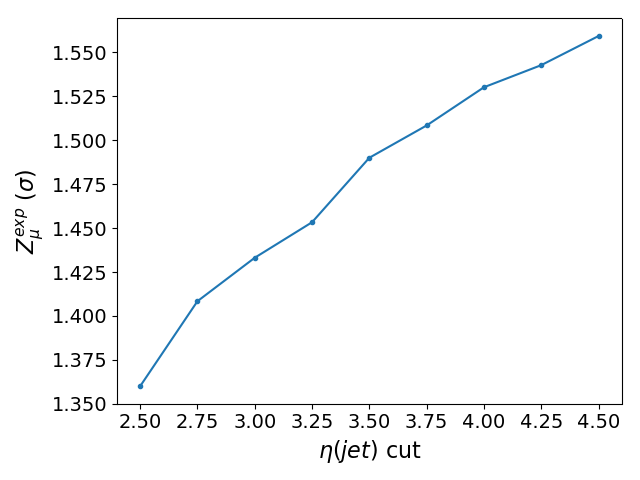
\includegraphics[width = 0.34\textwidth]{figures/signif_jetEta.png}
  	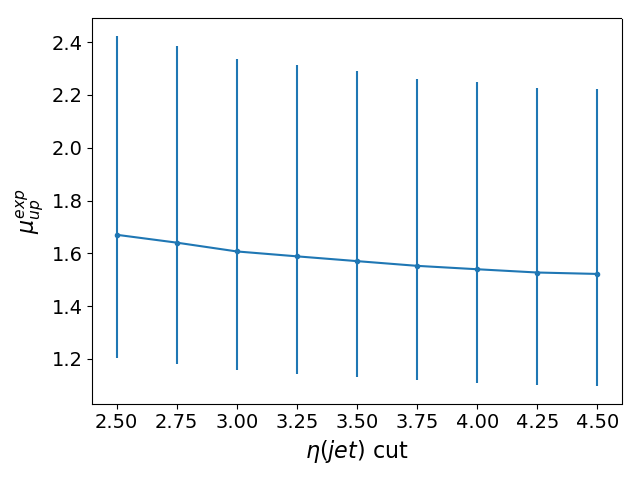
\includegraphics[width = 0.34\textwidth]{figures/exp_upper_jetEta.png}
  \centering
	\caption{\textbf{Left:} Expected significance ($Z_{\mu}^{exp}$) for different $\eta(jet)$ cuts is shown. The cuts applied on the $\eta(jet)$ are shown on the x-axis and corresponding expected significance from the likelihood fit is shown on the y-axis. \textbf{Right:} Expected upper limit ($\mu_{up}^{exp}$) for different $\eta(jet)$ cuts is shown. The cuts applied on the $\eta(jet)$ are shown on the x-axis and corresponding expected upper limits are shown on the y-axis. Error bars representing the total uncertainty on the expected upper limits are shown as vertical lines.}
	\label{fig:4lep-jetEta-optimisation}
\end{figure}


From Figure \ref{fig:4lep-jetEta-optimisation}, we can see that the $\eta(jet)$ cut which maximises the sensitivity of \tWZ in the tetralepton channel is requiring that $\eta(jet) < 4.5$. This selection criteria was set for the $\eta(jet)$ across all regions.\\\\


In Figure~\ref{fig:4lep-jetpt-optimisation} the expected significance ($Z_{\mu}^{exp}$) and expected upper limits ($\mu_{up}^{exp}$) for different $p_{T}(jet)$ cuts are shown.
\begin{figure}[h!]
	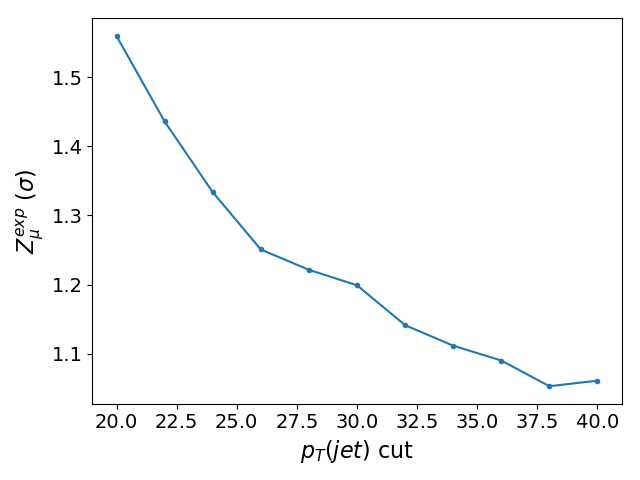
\includegraphics[width = 0.34\textwidth]{figures/signif_jetPt.png}
  	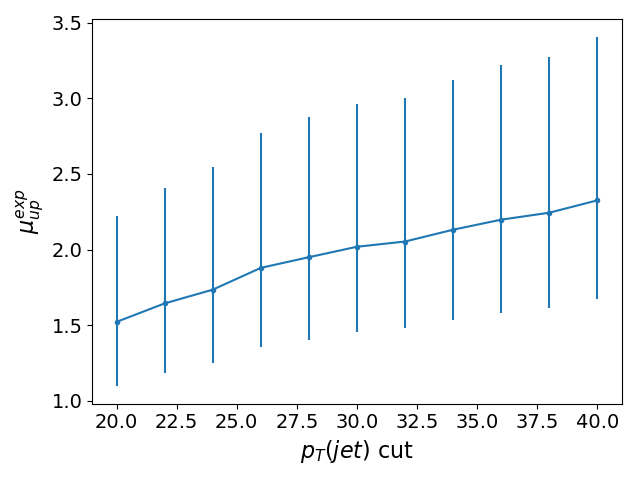
\includegraphics[width = 0.34\textwidth]{figures/exp_upper_jetPt.png}
  \centering
	\caption{\textbf{Left:} Expected significance ($Z_{\mu}^{exp}$) for different $p_{T}(jet)$ cuts is shown. The cuts applied on the $p_{T}(jet)$ are shown on the x-axis and corresponding expected significance from the likelihood fit is shown on the y-axis. \textbf{Right:} Expected upper limit ($\mu_{up}^{exp}$) for different $p_{T}(jet)$ cuts is shown. The cuts applied on the $p_{T}(jet)$ are shown on the x-axis and corresponding expected upper limits are shown on the y-axis. Error bars representing the total uncertainty on the expected upper limits are shown as vertical lines.}
		\label{fig:4lep-jetpt-optimisation}
\end{figure}


From Figure \ref{fig:4lep-jetpt-optimisation}, we can see that the $p_{T}(jet)$ cut which maximises the sensitivity of \tWZ is requiring that $p_{T}(jet) > 20$GeV. This selection criteria was set for the $p_{T}(jet)$ across all regions.\\\\

In Figure~\ref{fig:4lep-btagWP-optimization} the expected significance ($Z_{\mu}^{exp}$) and expected upper limits ($\mu_{up}^{exp}$) for a range of different configurations of DL1r $b$-tagged jet working points across different regions.
\begin{figure}[h!]
	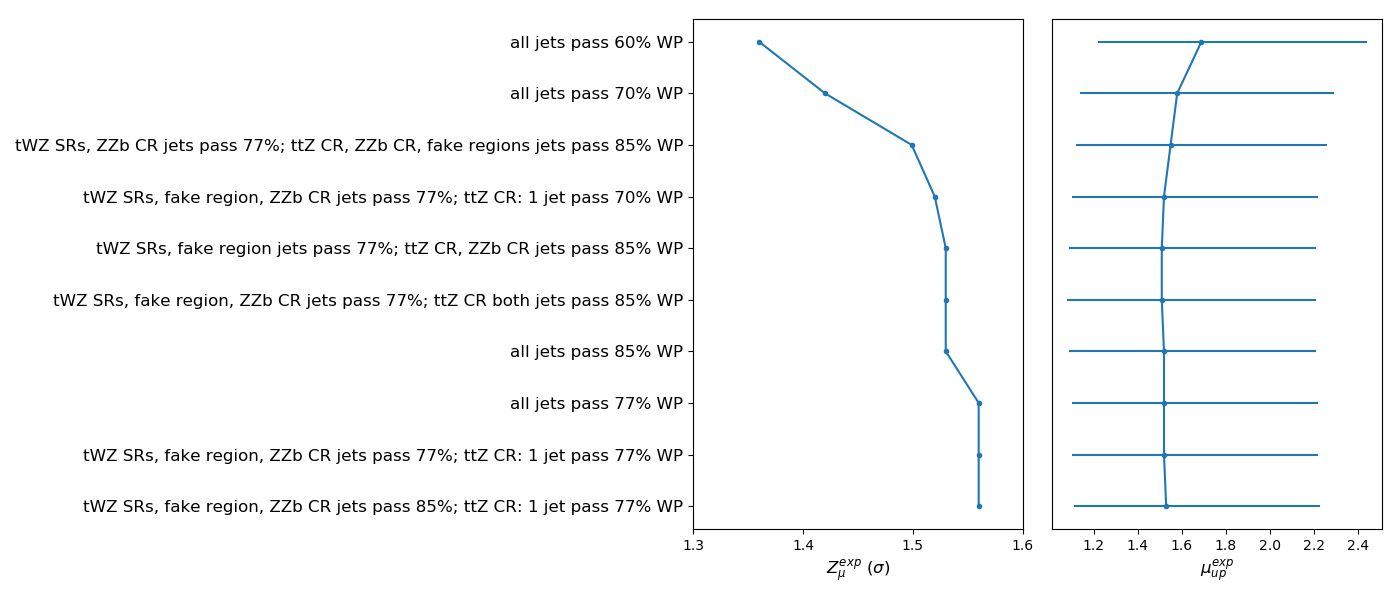
\includegraphics[width = 1\textwidth]{figures/btagWP_optimization.png}
  \centering
	\caption{Expected significance ($Z_{\mu}^{exp}$) and expected upper limit ($\mu_{up}^{exp}$) for different configurations of DL1r $b$-tagged jet working points is shown. The common y-axis shows the different configurations of DL1r $b$-tagged jet working points. On the left panel, the expected significance from the likelihood fit is shown on the x-axis. On the right panel, the expected upper limit from the likelihood fit is shown on the x-axis (with the corresponding total uncertainty represented by horizontal lines).}
	\label{fig:4lep-btagWP-optimization}
\end{figure}


From Figure \ref{fig:4lep-btagWP-optimization}, we can see that requiring that $b$-tagged jets pass the 77$\%$ DL1r WP in the \tWZ SR, $(tWZ)_{\text{fake}}$ CR and the $ZZb$ CR and that at least one $b$-tagged jet in the $t\bar{t}Z$ SR passes the 77$\%$ DL1r WP (the other jet is just required to pass the 85$\%$ DL1r WP) maximises the sensitivity overall (compared to the other investigated configurations). This configuration was chosen $b$-tagged jets.\\\\

The $p_{T}(\text{L Lepton})$ is constrained by the single lepton triggers (Table~\ref{tab:triggersummary}). We choose to apply a cut on the $p_{T}(\text{NL Lepton})$ slightly tighter than the tightest single lepton $p_{T}$ cut in the trigger. We can however, try optimising the $p_{T}(\text{NL Lepton})$ cut by comparing the expected significance and limit for a range of $p_{T}{\text{NL Lepton}}$ cuts to determine the cut which maximizes sensitivity.\\\\

In Figure~\ref{fig:4lep-NLlep-optimization} the expected significance ($Z_{\mu}^{exp}$) and expected upper limits ($\mu_{up}^{exp}$) for different $p_{T}(\text{NL Lepton})$ cuts is shown.
\begin{figure}[h!]
	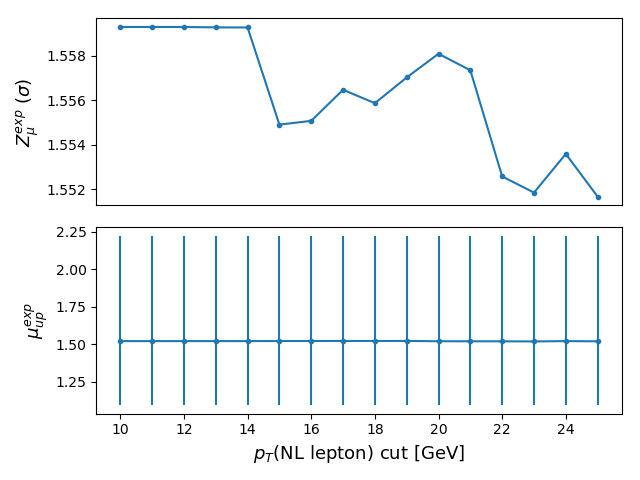
\includegraphics[width = 0.68\textwidth]{figures/NL_Lep_optimization.png}
  \centering
	\caption{Expected significance ($Z_{\mu}^{exp}$) and expected upper limit ($\mu_{up}^{exp}$) for different $p_{T}(\text{NL Lepton})$ cuts is shown. The common x-axis shows cut applied to the $p_{T}$ of the next-to-leading lepton. On the top panel, the expected significance from the likelihood fit is shown on the y-axis. On the bottom panel, the expected upper limit from the likelihood fit is shown on the y-axis (with the corresponding total uncertainty represented by vertical lines).}
	\label{fig:4lep-NLlep-optimization}
\end{figure}

Since there is a very small change between the different $p_{T}(\text{NL Lepton})$ cuts on the sensitivity of \tWZ, we choose to apply a $p_{T}(\text{NL Lepton})$ cut at 18 GeV, therefore applying a cut above the trigger $p_{T}$ cut to suppress any systematic from the modelling of the trigger efficiency.

\section{Signal and Control Regions}

In this section, pre-fit distributions of variables in each region are shown. More pre-fit distributions for each region are shown in the appendix (Section~\ref{sec:app-controlPlots}). For each figure in this section, the data is given by the black points and the MC predictions for each process are given by the histograms. The vertical lines on the data points represent the total uncertainty in the data and the diagonal lined bands represent the total MC uncertainty. The lower panel in each plot shows the ratios of the data to the theoretical predictions. The plots in the $tWZ$ OF SR and $tWZ$ SF SR are kept blinded by omitting the data points.\\\\

In Table~\ref{tab:4Lep-PreFit-Yields}, the pre-fit yields for each sample in each region is shown.
\begin{table}[h!]
\huge
    \resizebox{1\textwidth}{!}{%
\begin{tabular}{|ll|l|l|l|l|l|}
\hline
\multicolumn{2}{|l|}{}                                      & $tWZ$ OF SR                      & $tWZ$ SF SR                    & $t\bar{t}Z$ CR                      & $ZZb$ CR                      & $(tWZ)_{\text{fake}}$ CR       \\ \hline
\multicolumn{2}{|l|}{$t\bar{t}Z$}                                   & 13.9325 $\pm$ 1.84643         & 10.1343 $\pm$ 1.36039       & 31.7149 $\pm$ 4.46776      & 5.26303 $\pm$ 0.696828      & 19.1224 $\pm$ 2.50011      \\
\multicolumn{2}{|l|}{$t\bar{t}Z$ fakes}                             & 0.0687541 $\pm$ 0.0482172     & 0.032827 $\pm$ 0.026286     & 0.0709734 $\pm$ 0.043509   & 0.0474576 $\pm$ 0.0301512   & 4.94775 $\pm$ 2.48939      \\
\multicolumn{2}{|l|}{$tWZ$}                                   & 3.81359 $\pm$ 0.392241        & 2.57584 $\pm$ 0.326401      & 2.61991 $\pm$ 0.861557     & 1.4023 $\pm$ 0.156686       & 4.93485 $\pm$ 0.692143     \\
\multicolumn{2}{|l|}{$ZZ$}                                    & 0.546045 $\pm$ 0.18975        & 8.76232 $\pm$ 2.66871       & 1.22357 $\pm$ 0.376889     & 46.0616 $\pm$ 13.9203       & 7.76724 $\pm$ 2.36894      \\ \hline
\multicolumn{1}{|l|}{\multirow{9}{*}{other}} & $t\bar{t}$           & 6e-06 $\pm$ 3.04506e-06       & 0.250783 $\pm$ 0.44226      & 0.269883 $\pm$ 0.223373    & 6e-06 $\pm$ 3.04506e-06     & 2.36284 $\pm$ 0.927828     \\
\multicolumn{1}{|l|}{}                       & $tZq$          & 0.0827265 $\pm$ 0.0399222     & 0.0757694 $\pm$ 0.0355101   & 0.0637132 $\pm$ 0.0293762  & 0.0590199 $\pm$ 0.0244576   & 4.91371 $\pm$ 0.754695     \\
\multicolumn{1}{|l|}{}                       & $t\bar{t}W$ & 0.00674747 $\pm$ 0.00793546   & 0.00279491 $\pm$ 0.00287747 & 6e-06 $\pm$ 3.04506e-06    & 0.00221727 $\pm$ 0.00562041 & 0.944039 $\pm$ 0.296854    \\
\multicolumn{1}{|l|}{}                       & $WZ$        & 0.0439316 $\pm$ 0.0241635     & 0.0397876 $\pm$ 0.0154764   & 0.0134837 $\pm$ 0.0128327  & 0.0474188 $\pm$ 0.0330635   & 1.84471 $\pm$ 0.397076     \\
\multicolumn{1}{|l|}{}                       & $t\bar{t}t$          & 0.000987429 $\pm$ 0.000768187 & 0.00249801 $\pm$ 0.00138007 & 0.0141085 $\pm$ 0.00486102 & 6e-06 $\pm$ 3.04506e-06     & 0.0100745 $\pm$ 0.00367677 \\
\multicolumn{1}{|l|}{}                       & $t\bar{t}t\bar{t}$         & 0.00934516 $\pm$ 0.0080725    & 0.0107503 $\pm$ 0.00852049  & 0.0570846 $\pm$ 0.0206271  & 6e-06 $\pm$ 3.04506e-06     & 0.0216609 $\pm$ 0.00999533 \\
\multicolumn{1}{|l|}{}                       & $t\bar{t}WW$         & 0.0293456 $\pm$ 0.0263573     & 0.0296011 $\pm$ 0.0196075   & 0.26412 $\pm$ 0.0936908    & 0.013096 $\pm$ 0.0323943    & 0.151267 $\pm$ 0.0593376   \\
\multicolumn{1}{|l|}{}                       & $VVV (V = W/Z)$           & 0.280384 $\pm$ 0.0866421      & 0.191257 $\pm$ 0.0595588    & 0.0696624 $\pm$ 0.0228108  & 0.171171 $\pm$ 0.0526519    & 0.265957 $\pm$ 0.0821857   \\
\multicolumn{1}{|l|}{}                       & $t\bar{t}H$          & 0.854064 $\pm$ 0.177974       & 0.674566 $\pm$ 0.141771     & 1.98187 $\pm$ 0.406211     & 0.151447 $\pm$ 0.0357703    & 2.22981 $\pm$ 0.45726      \\ \hline
                                             & Total        & 19.6684 $\pm$ 1.95158         & 22.7832 $\pm$ 3.10338       & 38.3633 $\pm$ 4.6342       & 53.2187 $\pm$ 13.9618       & 49.5163 $\pm$ 4.77745      \\ \hline
                                             & data         & -                                         & -                                       & 36                                      & 49                                       & 57                                      \\ \hline
\end{tabular}}
\caption{The pre-fit yields for each sample in each region is shown.}
\label{tab:4Lep-PreFit-Yields}
\end{table}



\subsection{$tWZ$ OF SR}
\label{sec:controlplotstetralepton-tWZ-OF-SR}

%%%%%%%%%%%%%%%%%%%%%%%%%%%%%%%%%%%%
%%%%%%%%%%%%%%%%%%%%%%%%%%%%%%%%%%%%
%%%%%%%      tWZ OF region   %%%%%%%%%%
%%%%%%%%%%%%%%%%%%%%%%%%%%%%%%%%%%%%
%%%%%%%%%%%%%%%%%%%%%%%%%%%%%%%%%%%%

In this section, pre-fit distributions of variables in the $tWZ$ OF SR are shown. More pre-fit distributions for the $tWZ$ OF SR are shown in the appendix (Section \ref{sec:app-controlplotstetralepton-tWZ-OF-SR}).\\\\

In Figure~\ref{fig:4lep-OF-SR-leptonPlots} MC predictions for $p_{T}$, $\eta$ and $\phi$ for leading (L) leptons and next-to-leading (NL) leptons in the $tWZ$ OF SR region is shown.

\begin{figure}[htbp]
  \begin{tabular}{ccc}

    %%%%%%%%%%%%%%%
    %%% Leptons %%%
    %%%%%%%%%%%%%%%

    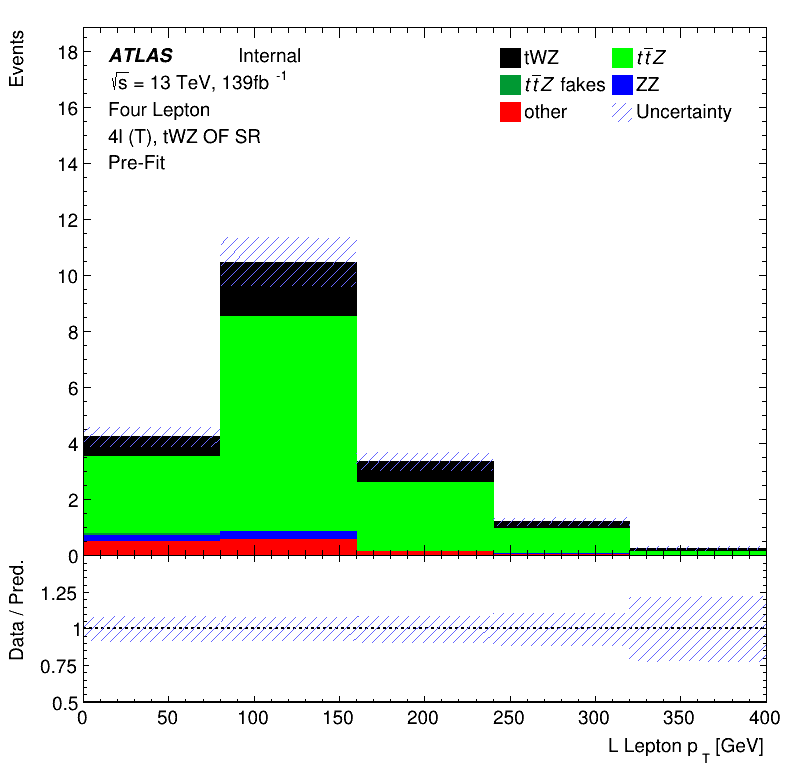
\includegraphics[width=.3\textwidth]{figures/PreFitPlots/lep4_tWZ_4T_OF_L_lepton_pt.png} &
    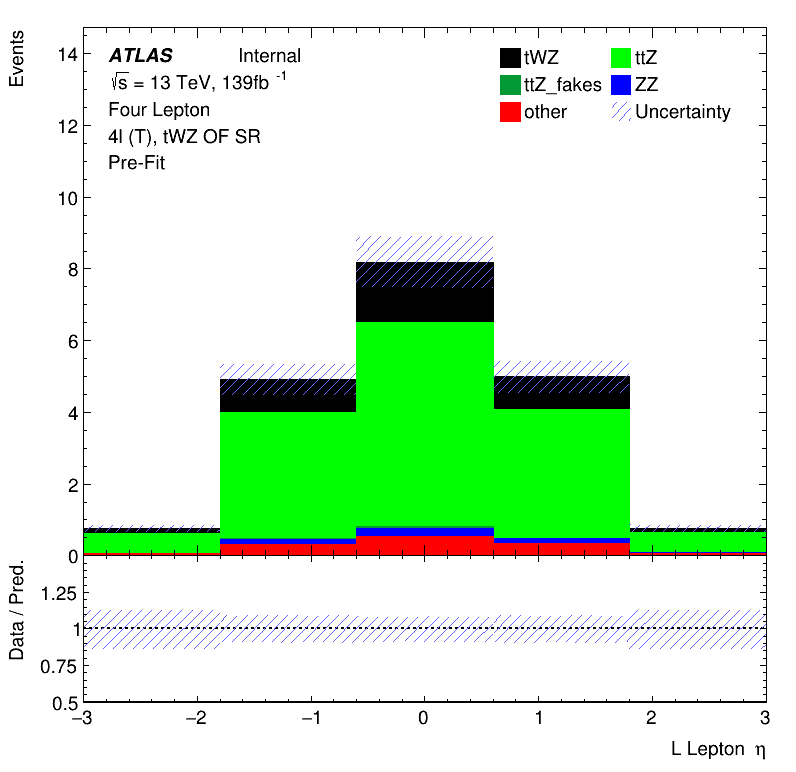
\includegraphics[width=.3\textwidth]{figures/PreFitPlots/lep4_tWZ_4T_OF_L_lepton_eta.png} &
    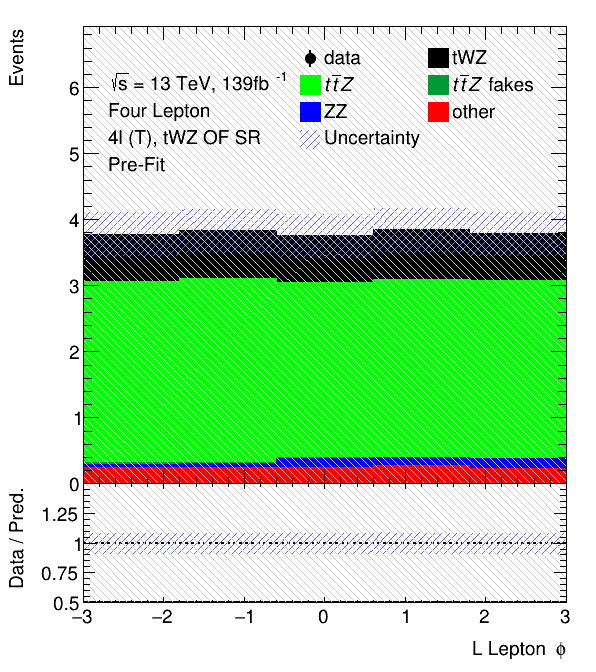
\includegraphics[width=.3\textwidth]{figures/PreFitPlots/lep4_tWZ_4T_OF_L_lepton_phi.png} \\
    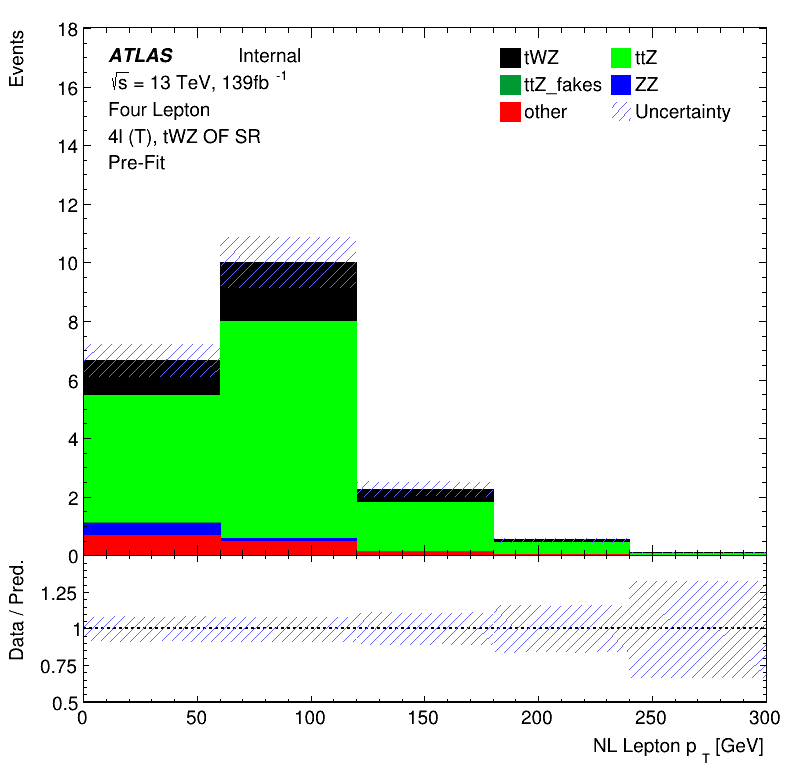
\includegraphics[width=.3\textwidth]{figures/PreFitPlots/lep4_tWZ_4T_OF_NL_lepton_pt.png} &
    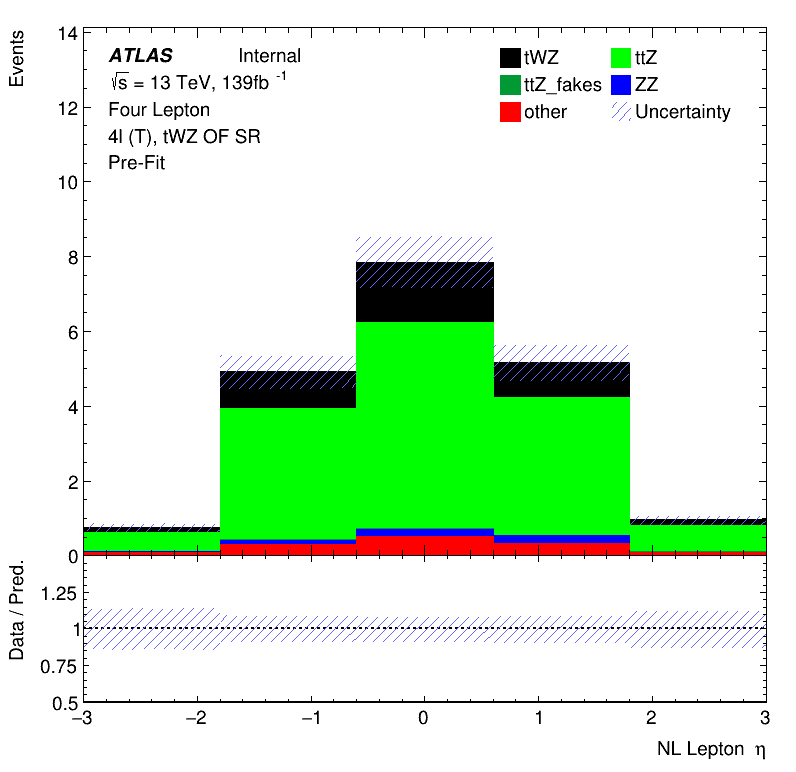
\includegraphics[width=.3\textwidth]{figures/PreFitPlots/lep4_tWZ_4T_OF_NL_lepton_eta.png} &
    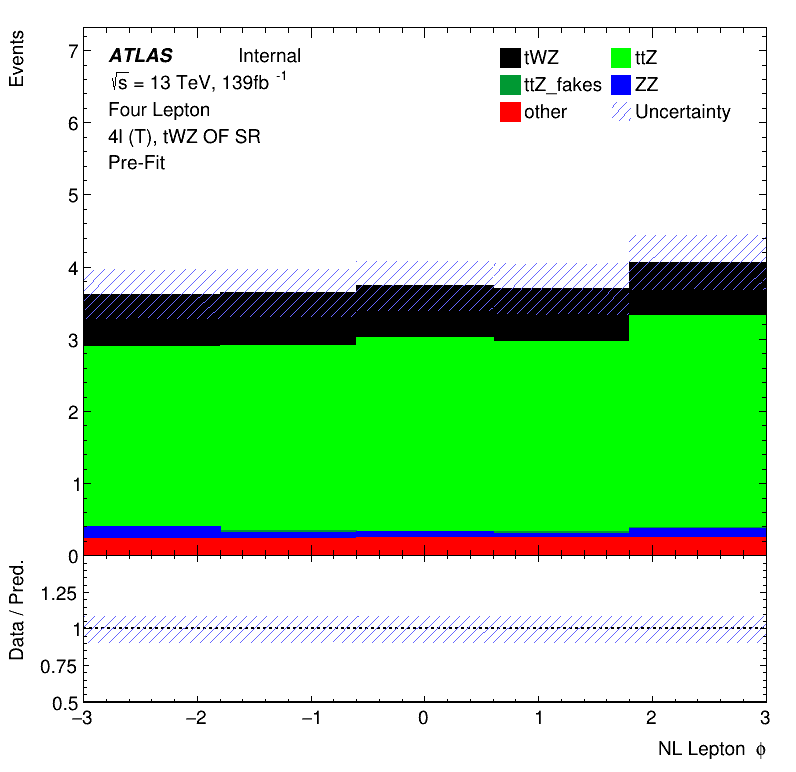
\includegraphics[width=.3\textwidth]{figures/PreFitPlots/lep4_tWZ_4T_OF_NL_lepton_phi.png} \\

  \end{tabular}
    \caption{MC predictions for $p_{T}$, $\eta$ and $\phi$ for leading (L) leptons (top row) and next-to-leading (NL) leptons (bottom row) in the $tWZ$ OF SR region (\textit{blinded}) is shown.}
  \label{fig:4lep-OF-SR-leptonPlots}
\end{figure}

In Figure~\ref{fig:4lep-OF-SR-LandNjetPlots} MC predictions for $p_{T}$, $\eta$ and $\phi$ for leading (L) jets and next-to-leading (NL) jets in the $tWZ$ OF SR region is shown.

\begin{figure}[htbp]
  \begin{tabular}{ccc}
    %%%%%%%%%%%%%%%%%
    %%%%% jets %%%%%
    %%%%%%%%%%%%%%%%%

    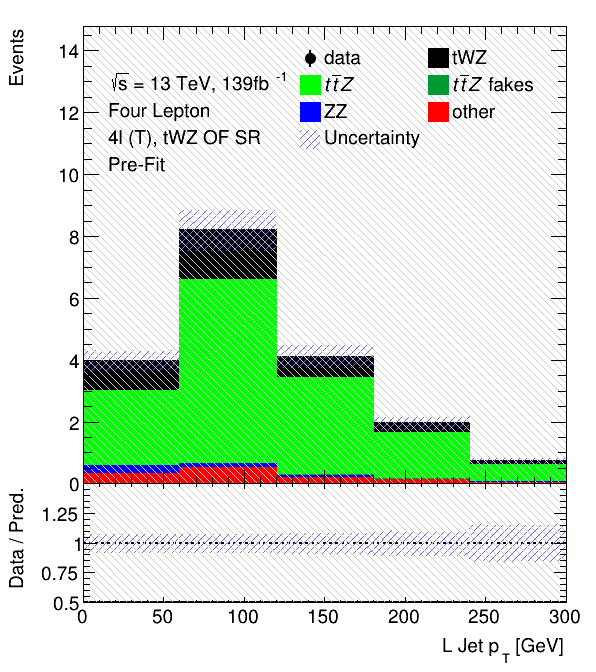
\includegraphics[width=.3\textwidth]{figures/PreFitPlots/lep4_tWZ_4T_OF_LJet_pt.png} &
    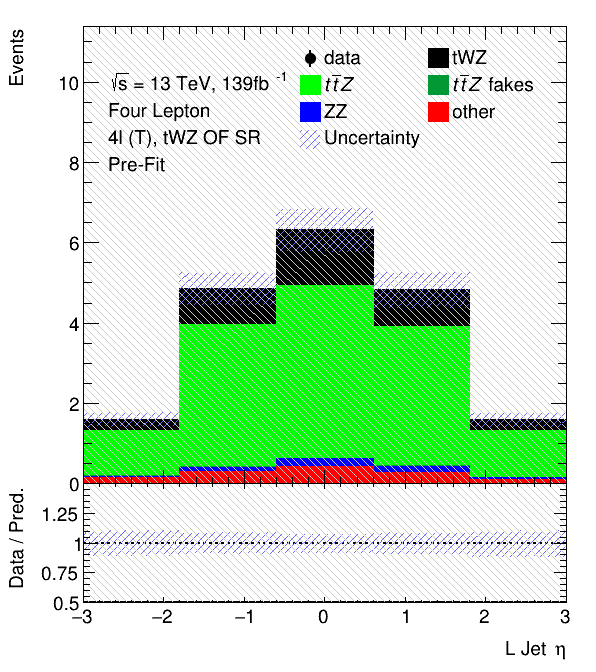
\includegraphics[width=.3\textwidth]{figures/PreFitPlots/lep4_tWZ_4T_OF_LJet_eta.png} &
    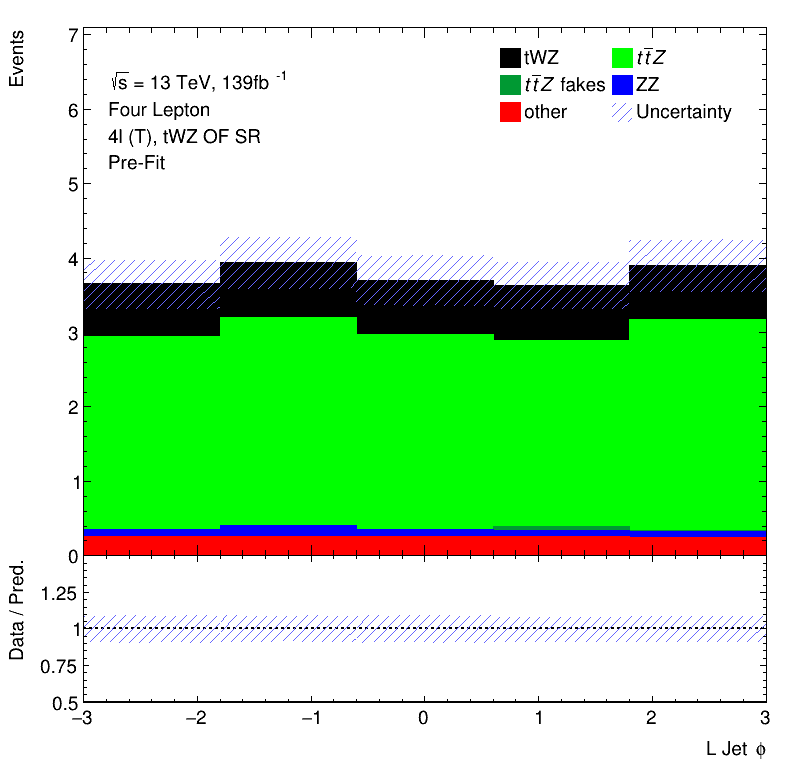
\includegraphics[width=.3\textwidth]{figures/PreFitPlots/lep4_tWZ_4T_OF_LJet_phi.png} \\
    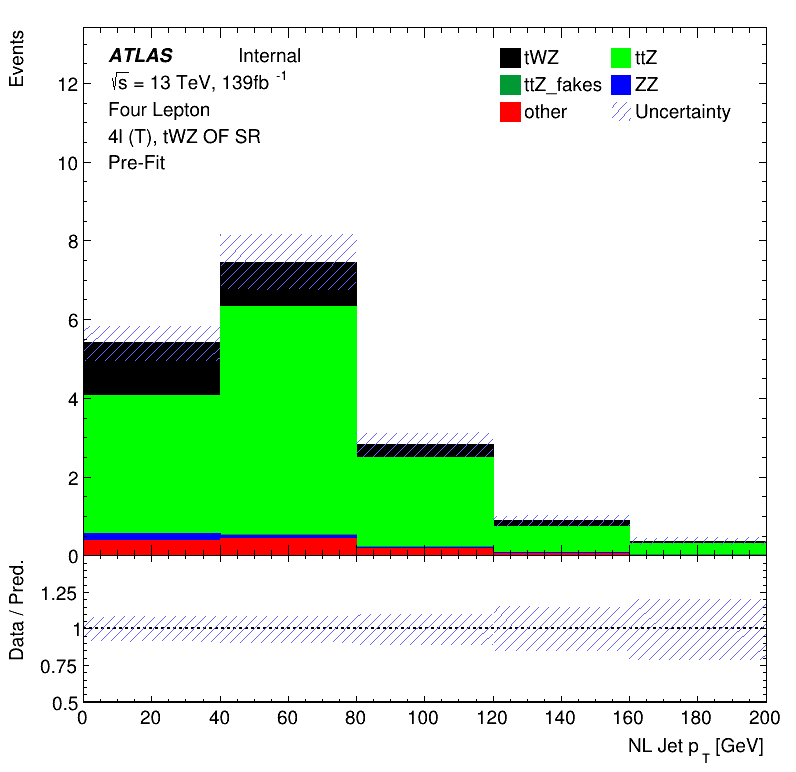
\includegraphics[width=.3\textwidth]{figures/PreFitPlots/lep4_tWZ_4T_OF_NLJet_pt.png} &
    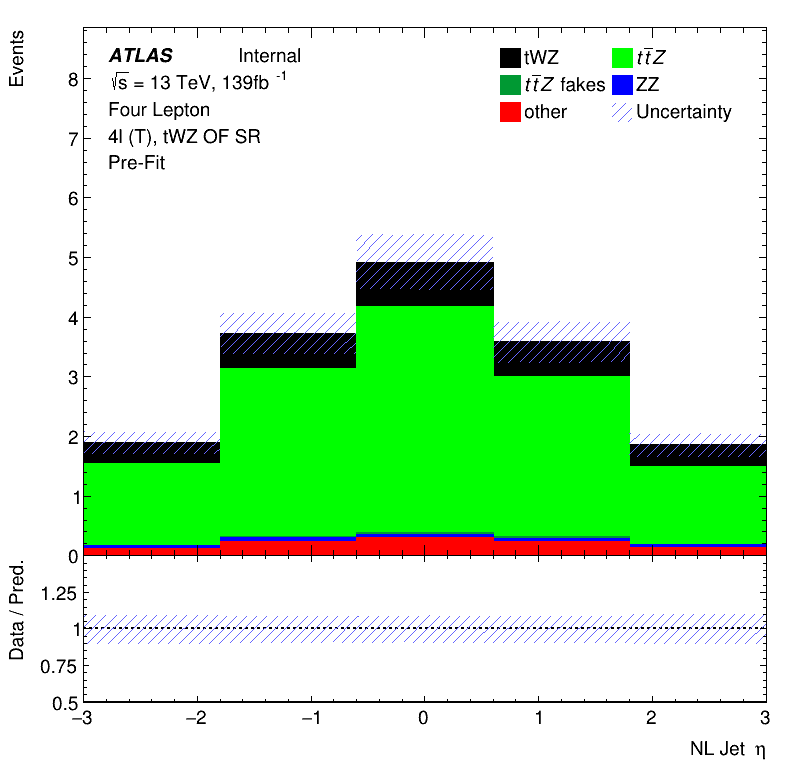
\includegraphics[width=.3\textwidth]{figures/PreFitPlots/lep4_tWZ_4T_OF_NLJet_eta.png} &
    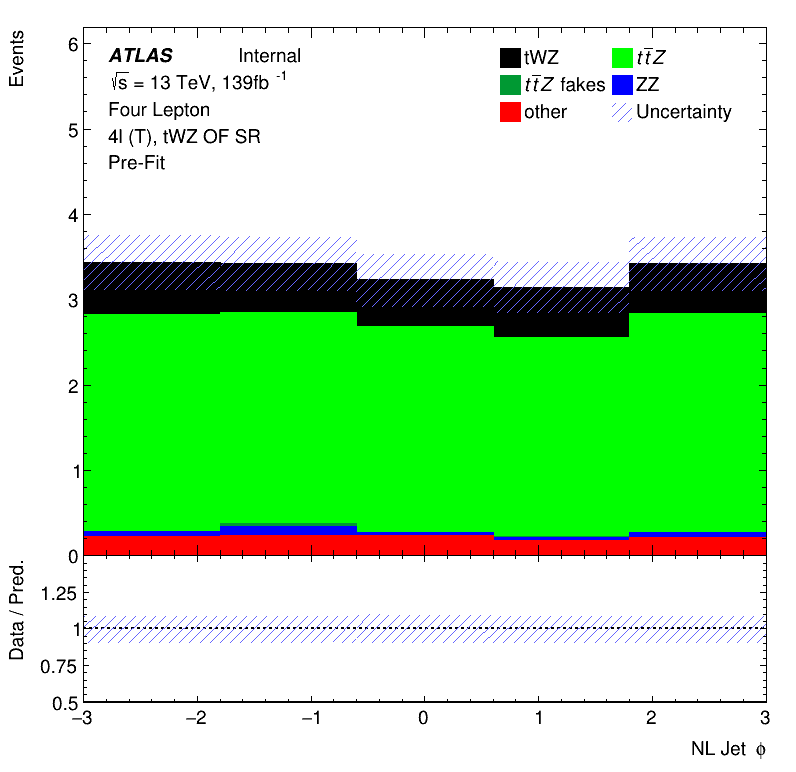
\includegraphics[width=.3\textwidth]{figures/PreFitPlots/lep4_tWZ_4T_OF_NLJet_phi.png} \\

  \end{tabular}
    \caption{MC predictions for $p_{T}$, $\eta$ and $\phi$ for leading (L) jets (top row) and next-to-leading (NL) jets (bottom row) in the $tWZ$ OF SR region (\textit{blinded}) is shown.}
    \label{fig:4lep-OF-SR-LandNjetPlots} 
\end{figure}

In Figure~\ref{fig:4lep-OF-SR-NNLjetPlots} MC predictions for $p_{T}$, $\eta$ and $\phi$ of the next-to-next-to-leading (NNL) jets, $H_{T}$ (scalar sum of Jet $p_{T}$) and the Number of jets in the $tWZ$ OF SR region is shown.


\begin{figure}[htbp]
 \centering

    %%%%%%%%%%%%%%%%%
    %%%%% jets %%%%%
    %%%%%%%%%%%%%%%%%

    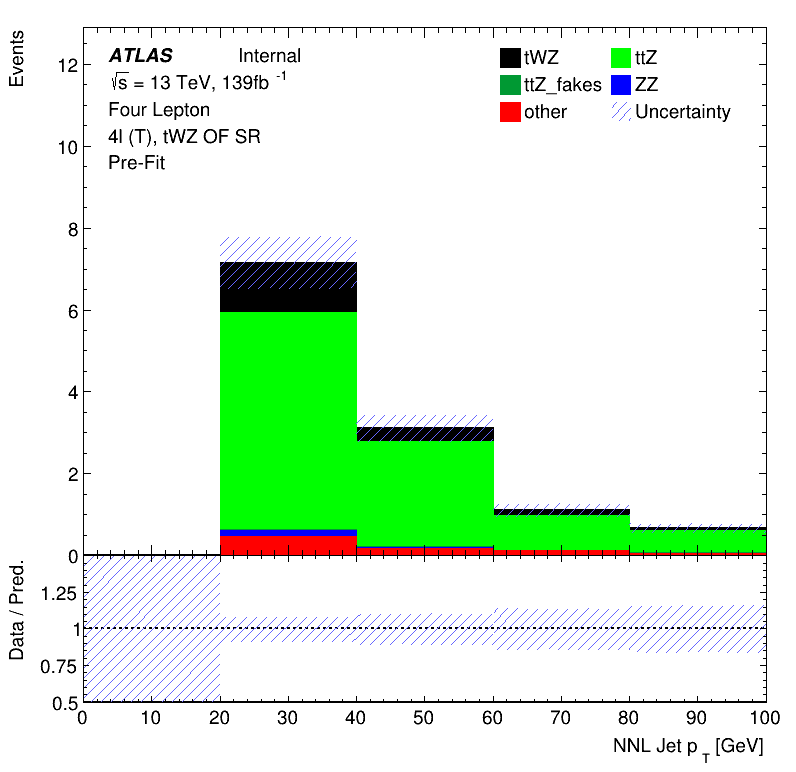
\includegraphics[width=.3\textwidth]{figures/PreFitPlots/lep4_tWZ_4T_OF_NNLJet_pt.png} \quad
    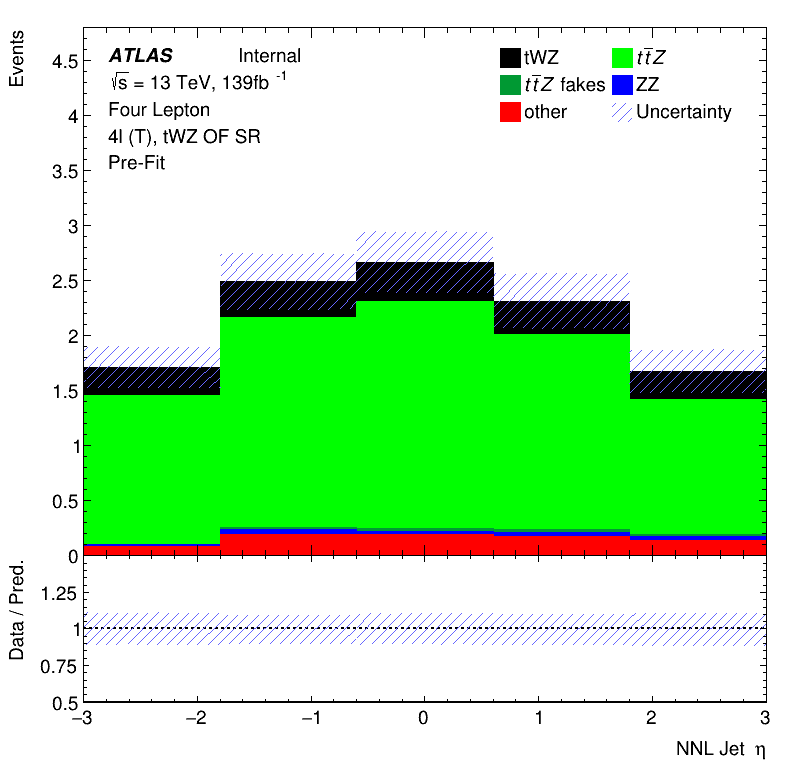
\includegraphics[width=.3\textwidth]{figures/PreFitPlots/lep4_tWZ_4T_OF_NNLJet_eta.png} \quad
    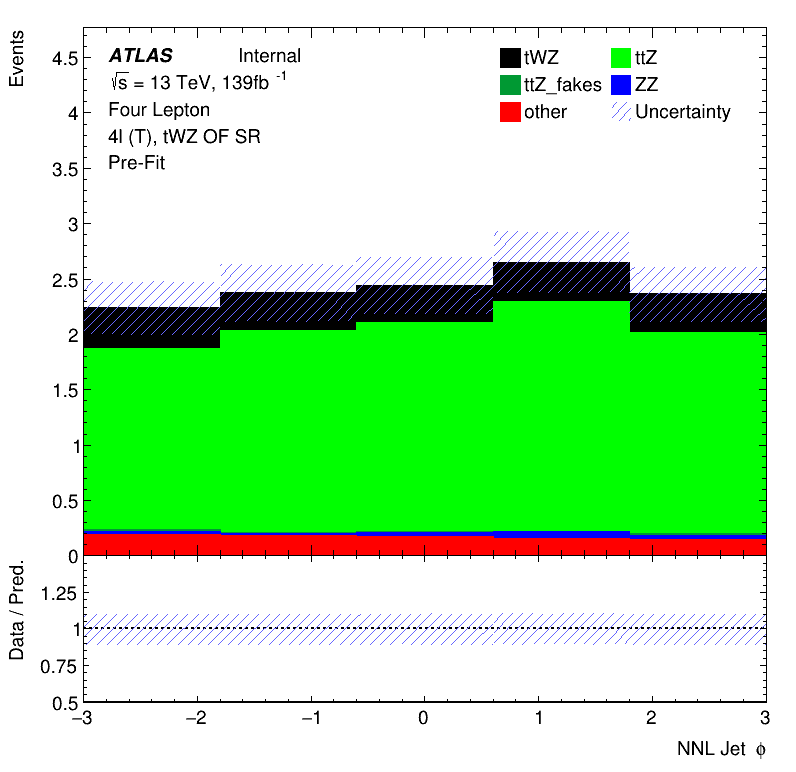
\includegraphics[width=.3\textwidth]{figures/PreFitPlots/lep4_tWZ_4T_OF_NNLJet_phi.png}

    \medskip

    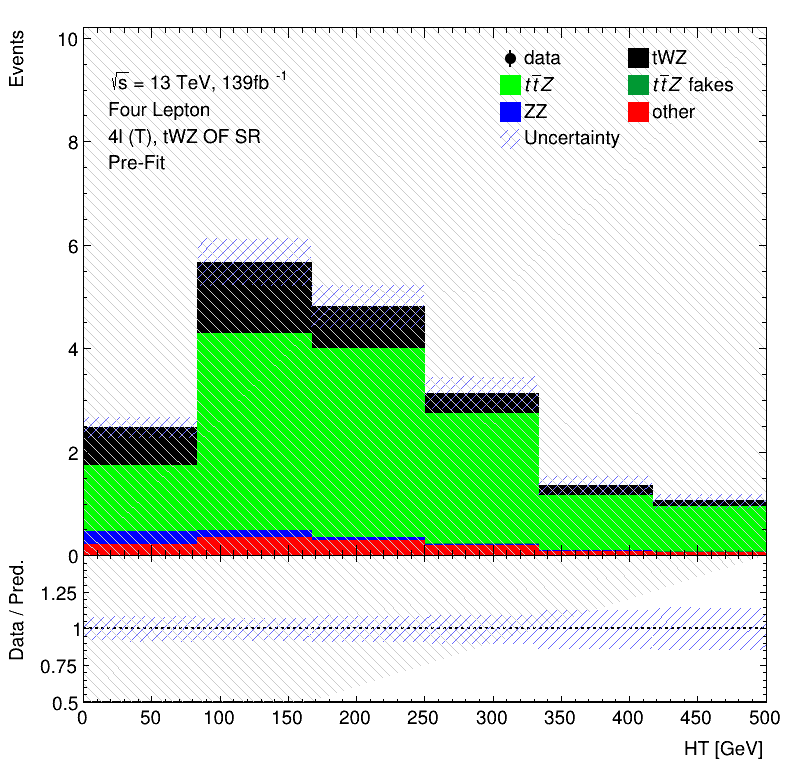
\includegraphics[width=.3\textwidth]{figures/PreFitPlots/lep4_tWZ_4T_OF_HT.png}   \quad
    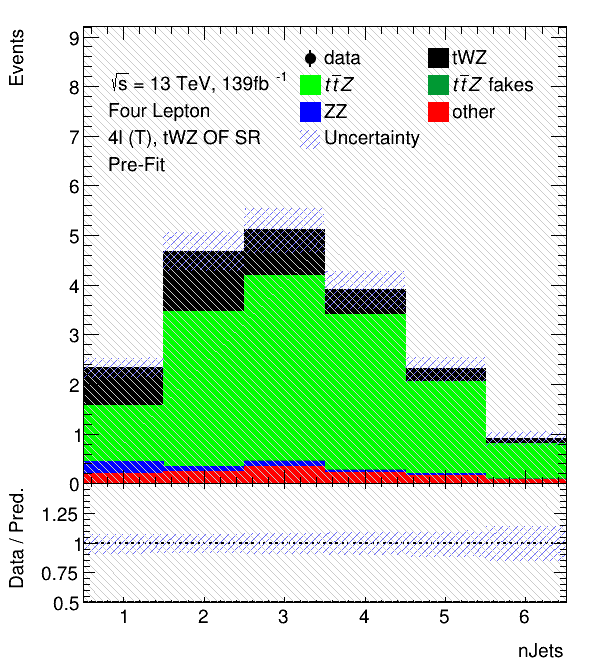
\includegraphics[width=.3\textwidth]{figures/PreFitPlots/lep4_tWZ_4T_OF_Num_Jets.png}

    \caption{\textbf{Top row:} MC predictions for $p_{T}$, $\eta$ and $\phi$ for next-to-next-to-leading (NNL) jets in the $tWZ$ OF SR region (\textit{blinded}) is shown. \textbf{Bottom row:} MC predictions for $H_{T}$ (scalar sum of Jet $p_{T}$) (left) and the Number of jets (right) in the $tWZ$ OF SR region (\textit{blinded}) is shown.}
    \label{fig:4lep-OF-SR-NNLjetPlots} 
\end{figure}



In Figure~\ref{fig:4lep-OF-SR-bjetPlots} MC predictions for $p_{T}$, $\eta$ and $\phi$ of the leading b-tagged jets, the scalar sum of b-tagged jet $p_{T}$ and the Number of b-tagged jets in the $tWZ$ OF SR region is shown.
\begin{figure}[htbp]
\centering
    %%%%%%%%%%%%%%%%%%
    %%%%% b jets %%%%%
    %%%%%%%%%%%%%%%%%%

    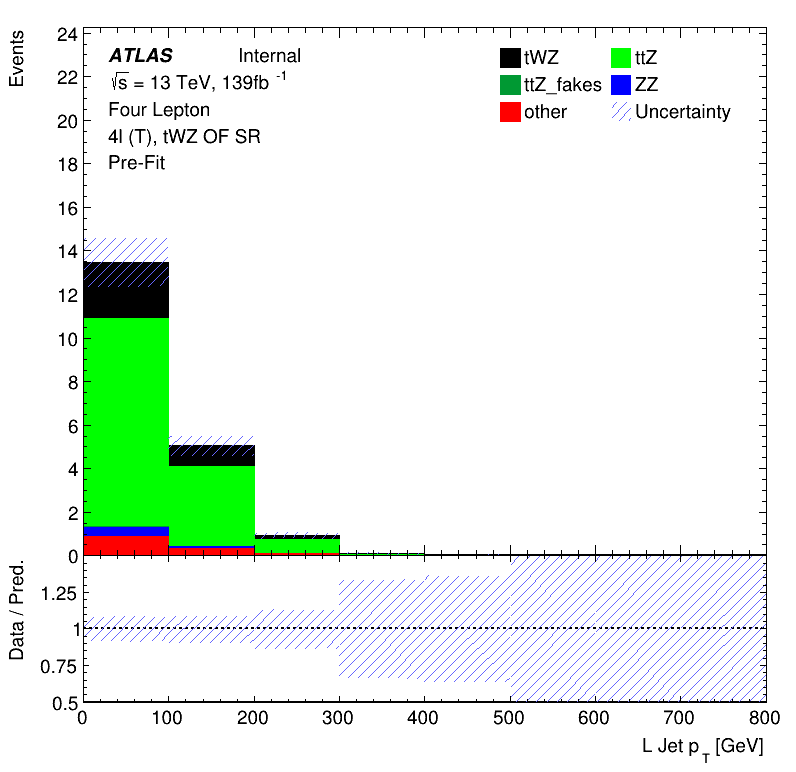
\includegraphics[width=.3\textwidth]{figures/PreFitPlots/lep4_tWZ_4T_OF_0_bJet_pt.png}   \quad
    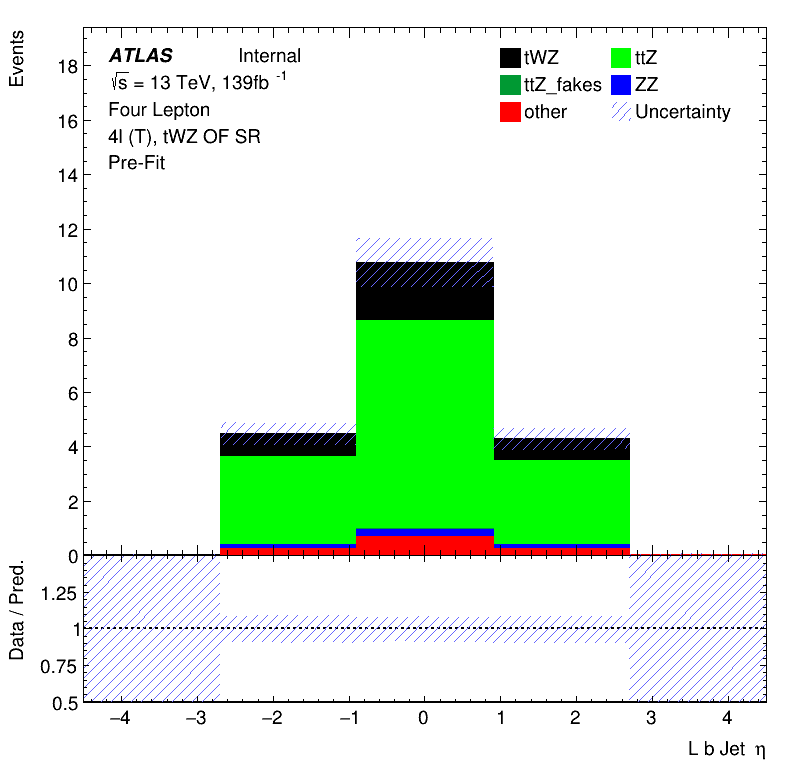
\includegraphics[width=.3\textwidth]{figures/PreFitPlots/lep4_tWZ_4T_OF_0_bJet_eta.png}    \quad
    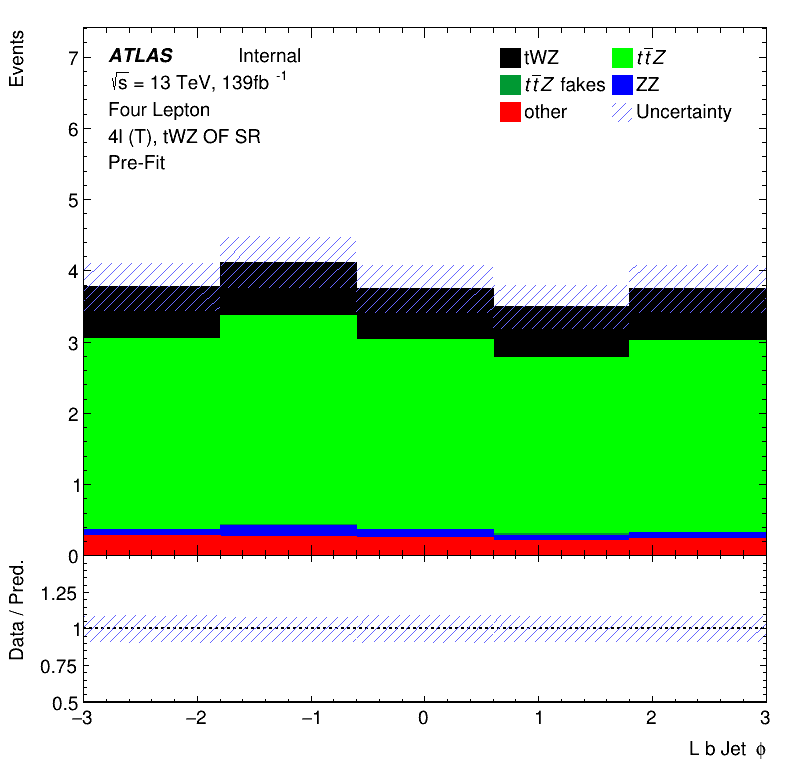
\includegraphics[width=.3\textwidth]{figures/PreFitPlots/lep4_tWZ_4T_OF_0_bJet_phi.png}

    \medskip

    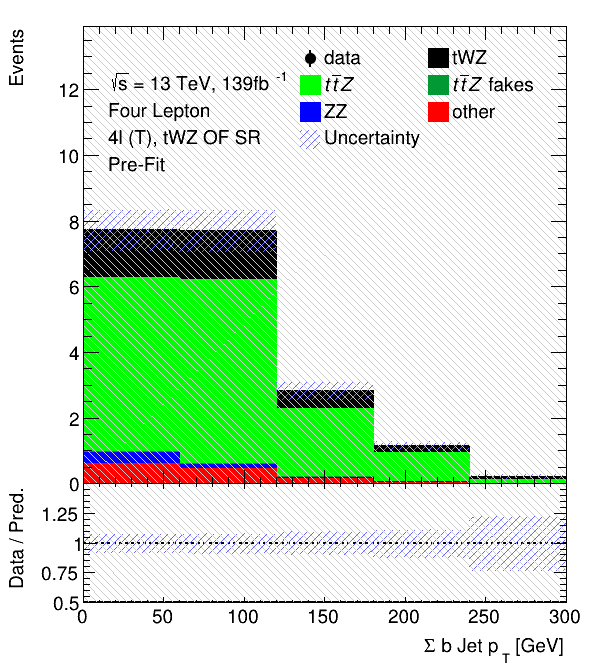
\includegraphics[width=.3\textwidth]{figures/PreFitPlots/lep4_tWZ_4T_OF_sum_bJet_Pt.png}  \quad
    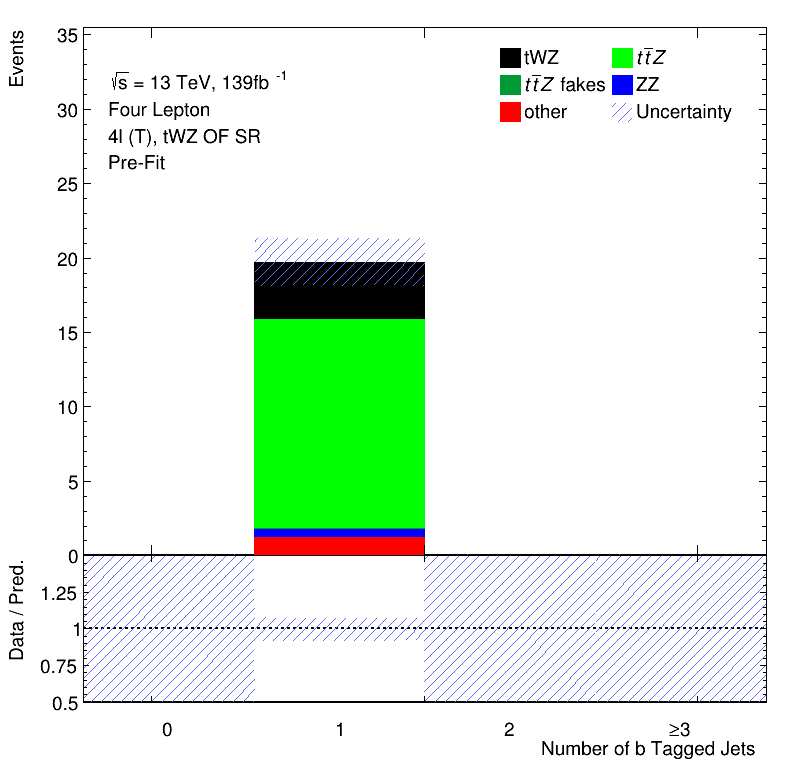
\includegraphics[width=.3\textwidth]{figures/PreFitPlots/lep4_tWZ_4T_OF_Num_bJets.png}

    \caption{\textbf{Top row:} MC predictions for $p_{T}$, $\eta$ and $\phi$ for leading b-tagged jets in the $tWZ$ OF SR region (\textit{blinded}) is shown. \textbf{Bottom row:} MC predictions for the scalar sum of b-tagged jet $p_{T}$ (left) and the Number of b-tagged jets (right) in the $tWZ$ OF SR region (\textit{blinded}) is shown.}
  \label{fig:4lep-OF-SR-bjetPlots}
\end{figure}


\subsection{$tWZ$ SF SR}
\label{sec:controlplotstetralepton-tWZ-SF-SR}

%%%%%%%%%%%%%%%%%%%%%%%%%%%%%%%%%%%%
%%%%%%%%%%%%%%%%%%%%%%%%%%%%%%%%%%%%
%%%%%%%      tWZ SF region   %%%%%%%%%%
%%%%%%%%%%%%%%%%%%%%%%%%%%%%%%%%%%%%
%%%%%%%%%%%%%%%%%%%%%%%%%%%%%%%%%%%%

In this section, pre-fit distributions of variables in the $tWZ$ SF SR are shown. More pre-fit distributions for the $tWZ$ SF SR are shown in the appendix (Section \ref{sec:app-controlplotstetralepton-tWZ-SF-SR}).\\\\

In Figure~\ref{fig:4lep-SF-SR-leptonPlots} MC predictions for $p_{T}$, $\eta$ and $\phi$ for leading (L) leptons and next-to-leading (NL) leptons in the $tWZ$ SF SR region is shown.

\begin{figure}[htbp]
  \begin{tabular}{ccc}

    %%%%%%%%%%%%%%%
    %%% Leptons %%%
    %%%%%%%%%%%%%%%

    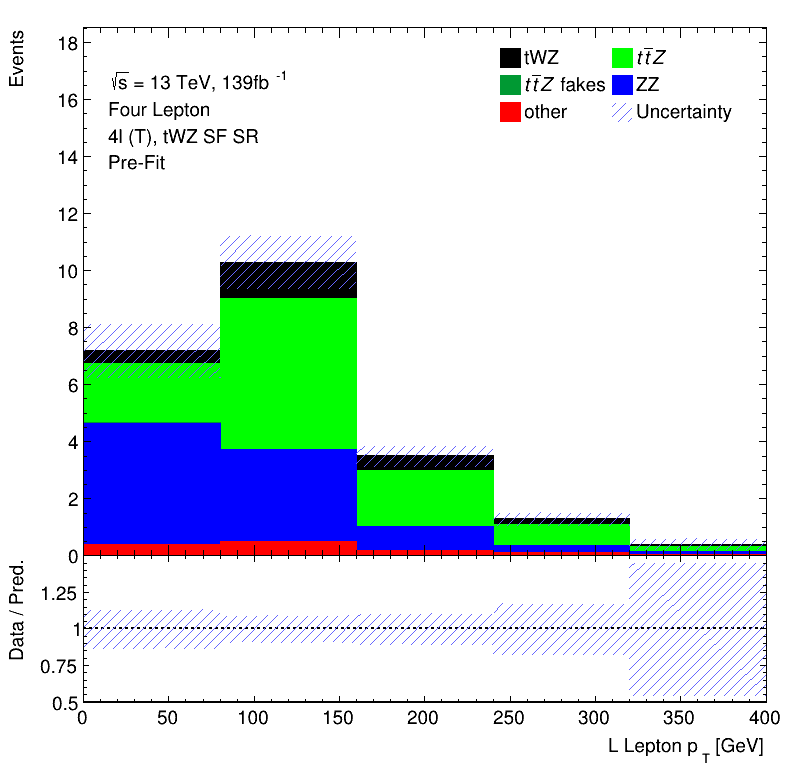
\includegraphics[width=.3\textwidth]{figures/PreFitPlots/lep4_tWZ_4T_SF_L_lepton_pt.png} &
    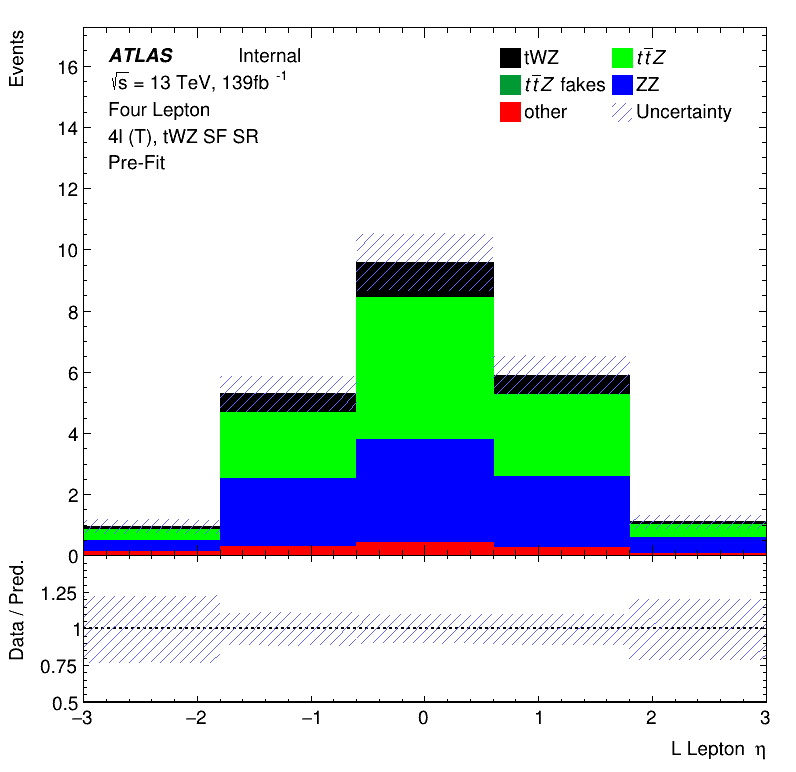
\includegraphics[width=.3\textwidth]{figures/PreFitPlots/lep4_tWZ_4T_SF_L_lepton_eta.png} &
    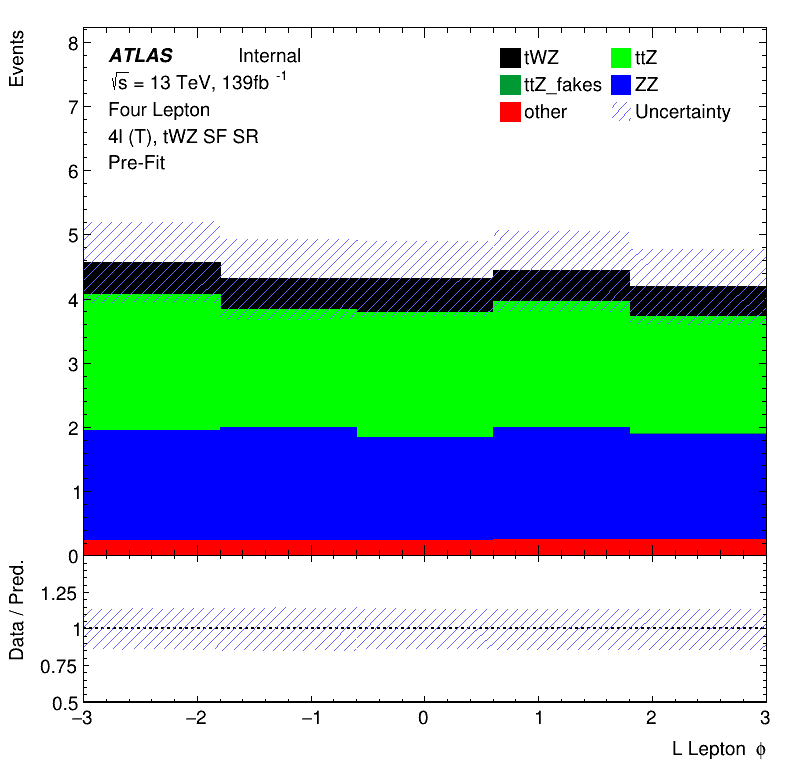
\includegraphics[width=.3\textwidth]{figures/PreFitPlots/lep4_tWZ_4T_SF_L_lepton_phi.png} \\
    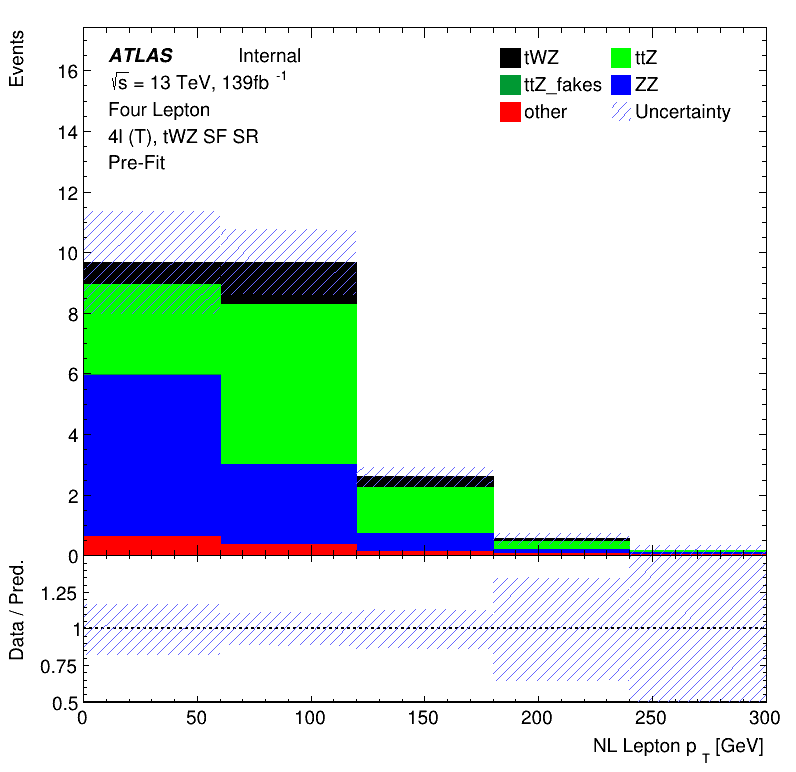
\includegraphics[width=.3\textwidth]{figures/PreFitPlots/lep4_tWZ_4T_SF_NL_lepton_pt.png} &
    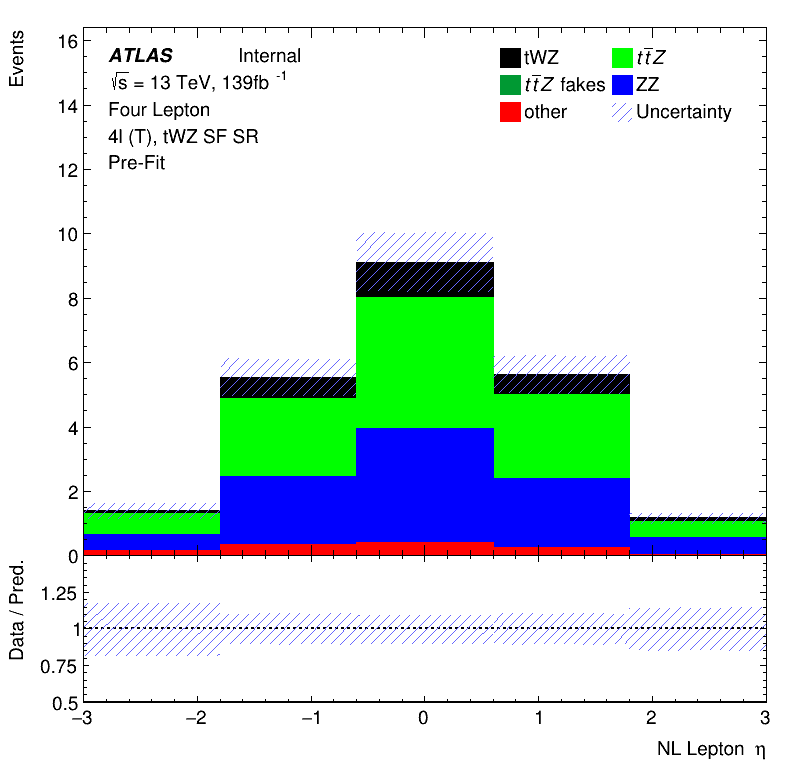
\includegraphics[width=.3\textwidth]{figures/PreFitPlots/lep4_tWZ_4T_SF_NL_lepton_eta.png} &
    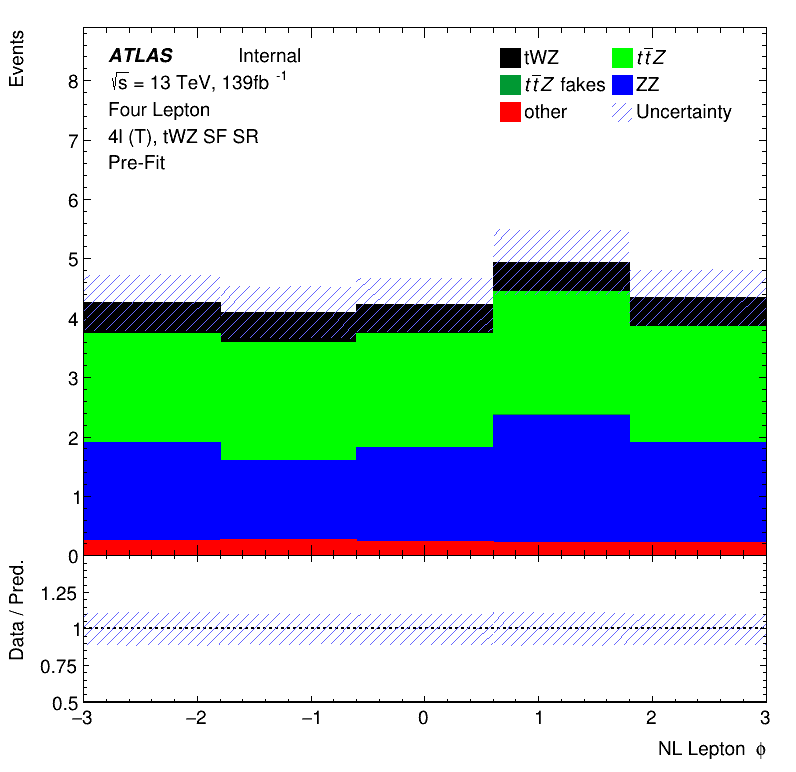
\includegraphics[width=.3\textwidth]{figures/PreFitPlots/lep4_tWZ_4T_SF_NL_lepton_phi.png} \\

  \end{tabular}
    \caption{MC predictions for $p_{T}$, $\eta$ and $\phi$ for leading (L) leptons (top row) and next-to-leading (NL) leptons (bottom row) in the $tWZ$ SF SR region (\textit{blinded}) is shown.}
  \label{fig:4lep-SF-SR-leptonPlots}
\end{figure}

In Figure~\ref{fig:4lep-SF-SR-LandNjetPlots} MC predictions for $p_{T}$, $\eta$ and $\phi$ for leading (L) jets and next-to-leading (NL) jets in the $tWZ$ SF SR region is shown.

\begin{figure}[htbp]
  \begin{tabular}{ccc}
    %%%%%%%%%%%%%%%%%
    %%%%% jets %%%%%
    %%%%%%%%%%%%%%%%%

    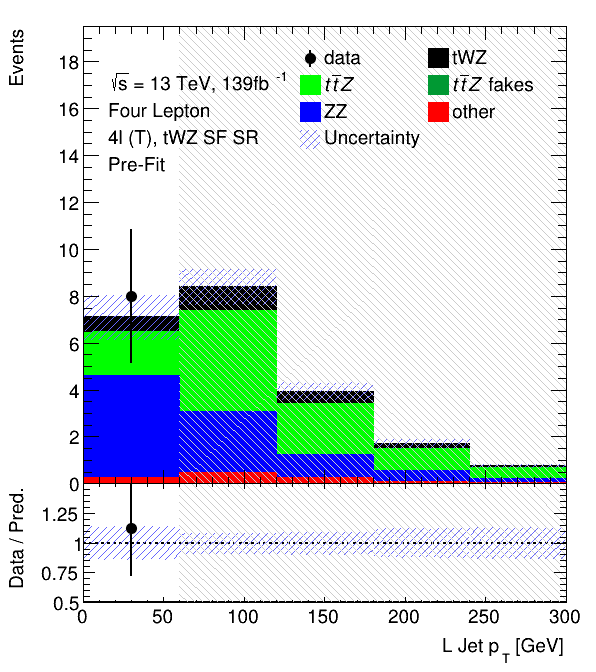
\includegraphics[width=.3\textwidth]{figures/PreFitPlots/lep4_tWZ_4T_SF_LJet_pt.png} &
    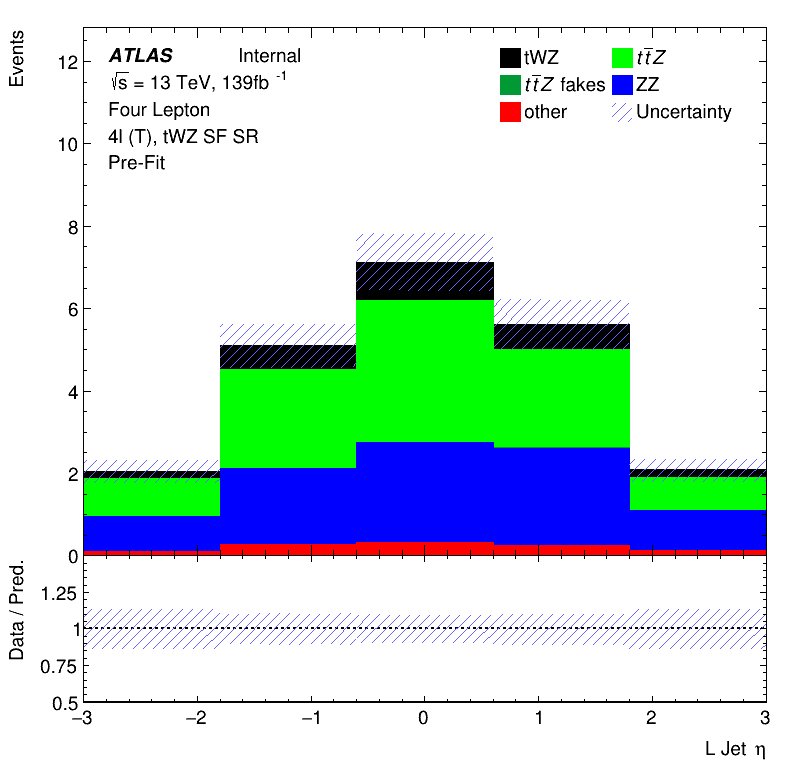
\includegraphics[width=.3\textwidth]{figures/PreFitPlots/lep4_tWZ_4T_SF_LJet_eta.png} &
    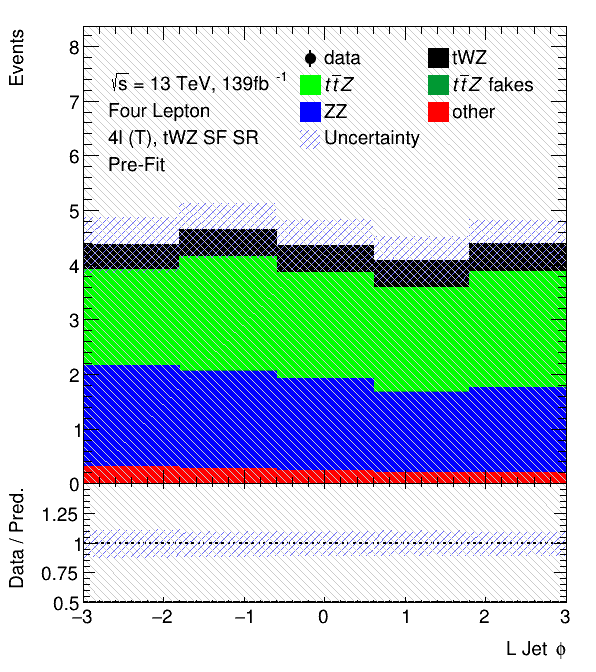
\includegraphics[width=.3\textwidth]{figures/PreFitPlots/lep4_tWZ_4T_SF_LJet_phi.png} \\
    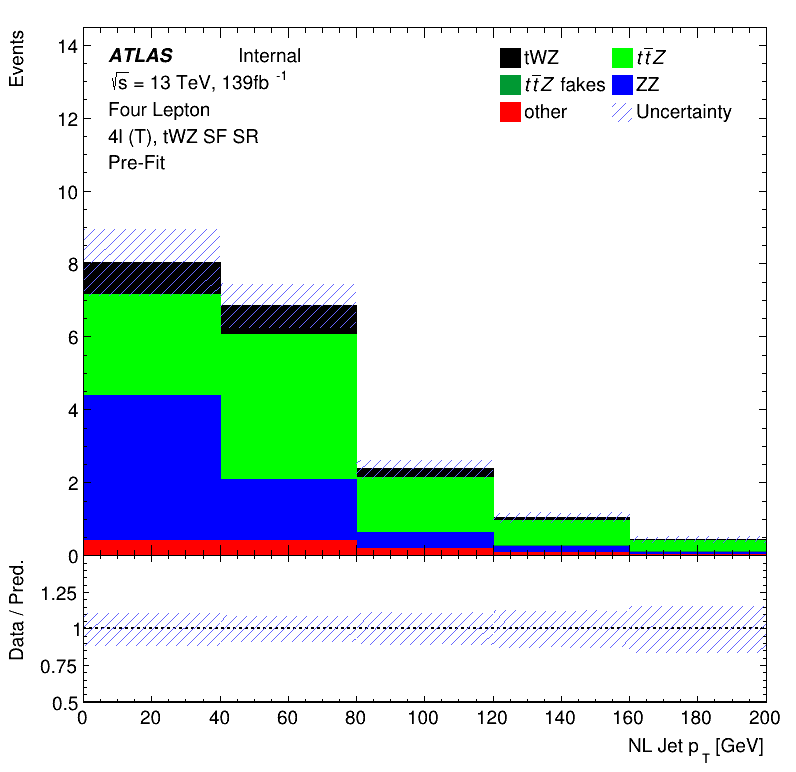
\includegraphics[width=.3\textwidth]{figures/PreFitPlots/lep4_tWZ_4T_SF_NLJet_pt.png} &
    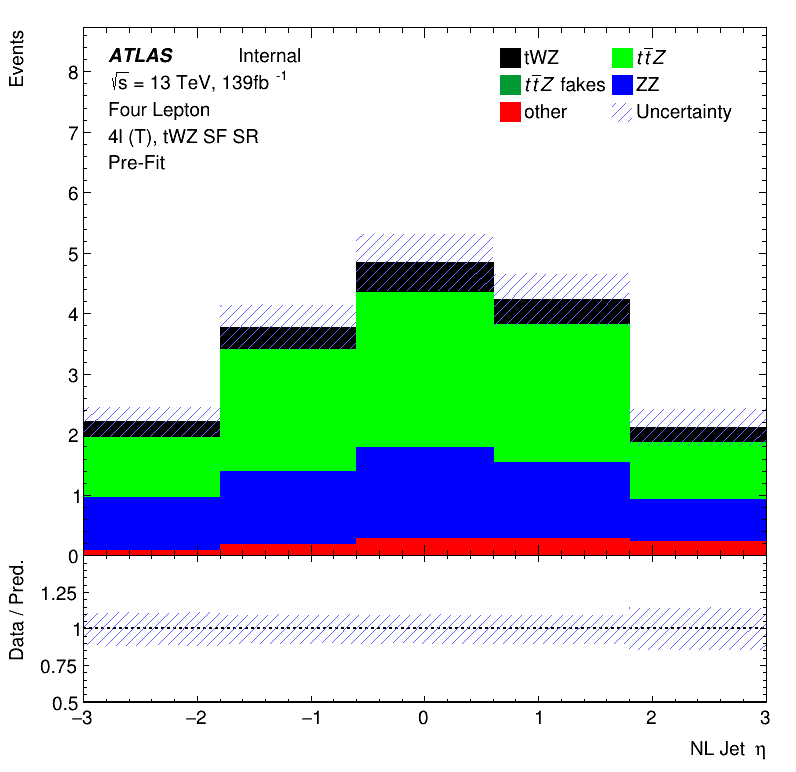
\includegraphics[width=.3\textwidth]{figures/PreFitPlots/lep4_tWZ_4T_SF_NLJet_eta.png} &
    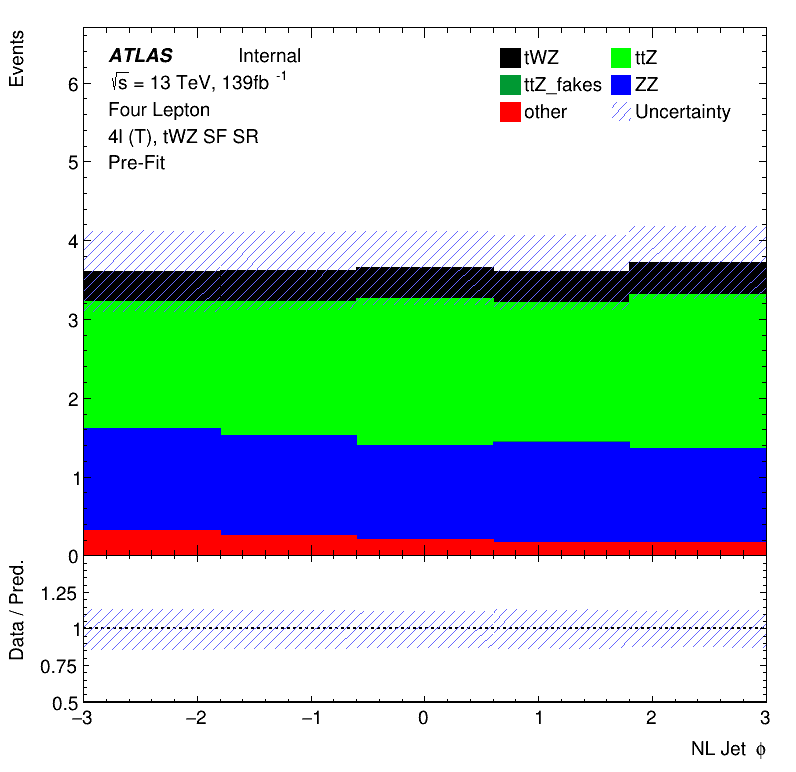
\includegraphics[width=.3\textwidth]{figures/PreFitPlots/lep4_tWZ_4T_SF_NLJet_phi.png} \\

  \end{tabular}
    \caption{MC predictions for $p_{T}$, $\eta$ and $\phi$ for leading (L) jets (top row) and next-to-leading (NL) jets (bottom row) in the $tWZ$ SF SR region (\textit{blinded}) is shown.}
    \label{fig:4lep-SF-SR-LandNjetPlots} 
\end{figure}

In Figure~\ref{fig:4lep-SF-SR-NNLjetPlots} MC predictions for $p_{T}$, $\eta$ and $\phi$ of the next-to-next-to-leading (NNL) jets, $H_{T}$ (scalar sum of Jet $p_{T}$) and the Number of jets in the $tWZ$ SF SR region is shown.


\begin{figure}[htbp]
 \centering

    %%%%%%%%%%%%%%%%%
    %%%%% jets %%%%%
    %%%%%%%%%%%%%%%%%

    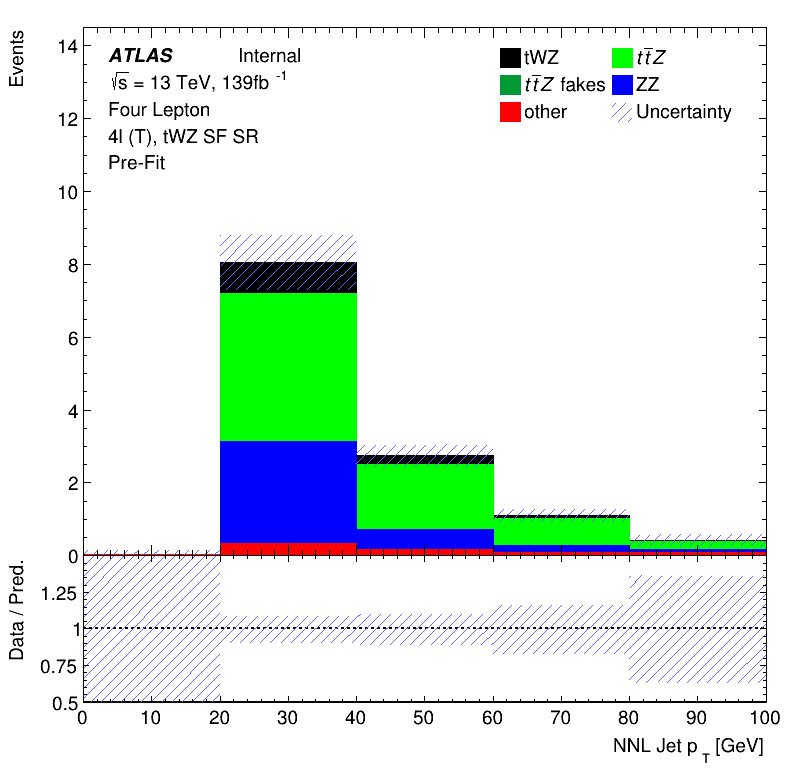
\includegraphics[width=.3\textwidth]{figures/PreFitPlots/lep4_tWZ_4T_SF_NNLJet_pt.png} \quad
    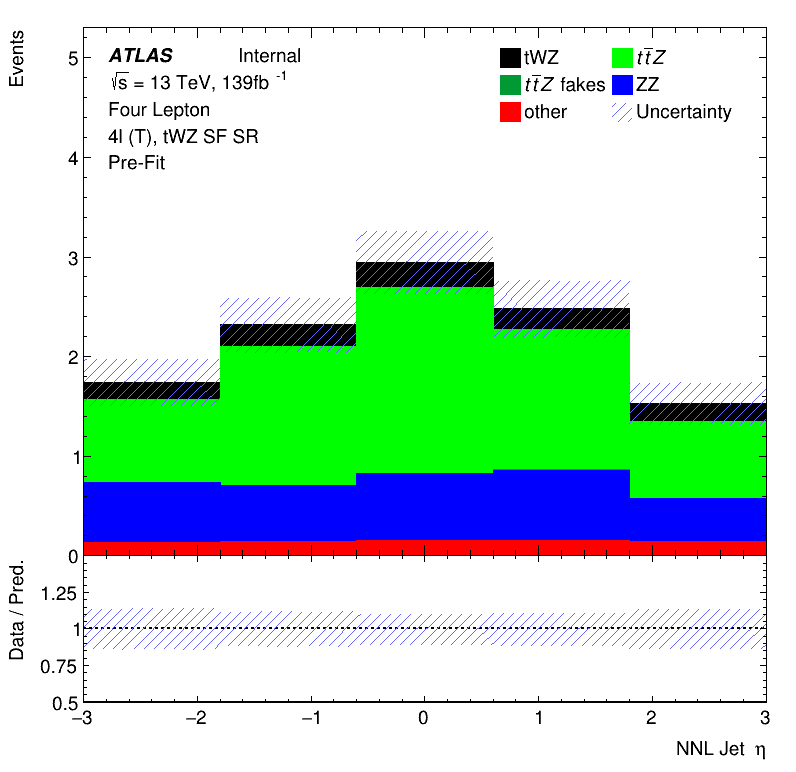
\includegraphics[width=.3\textwidth]{figures/PreFitPlots/lep4_tWZ_4T_SF_NNLJet_eta.png} \quad
    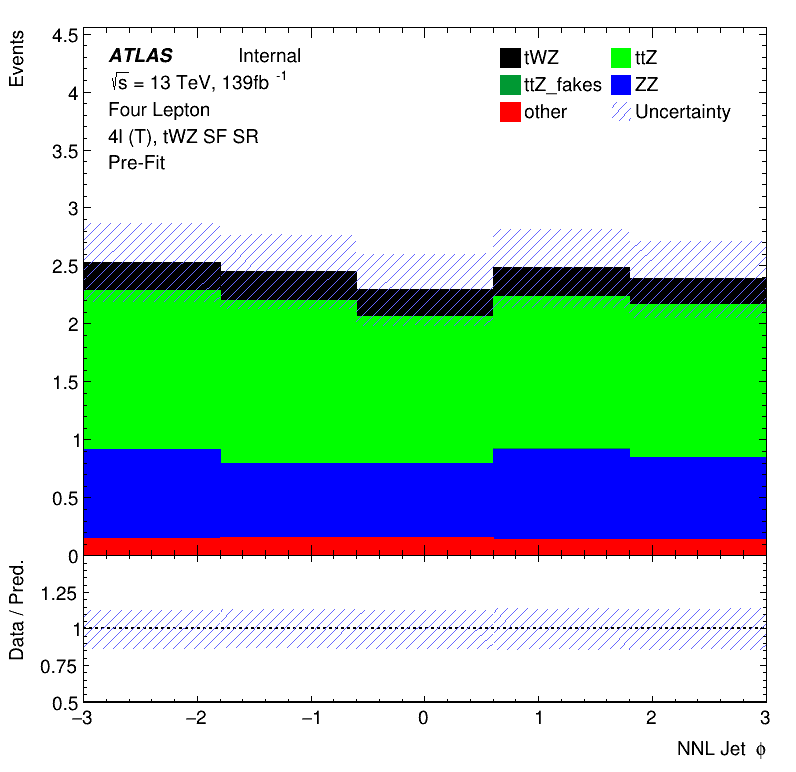
\includegraphics[width=.3\textwidth]{figures/PreFitPlots/lep4_tWZ_4T_SF_NNLJet_phi.png}

    \medskip

    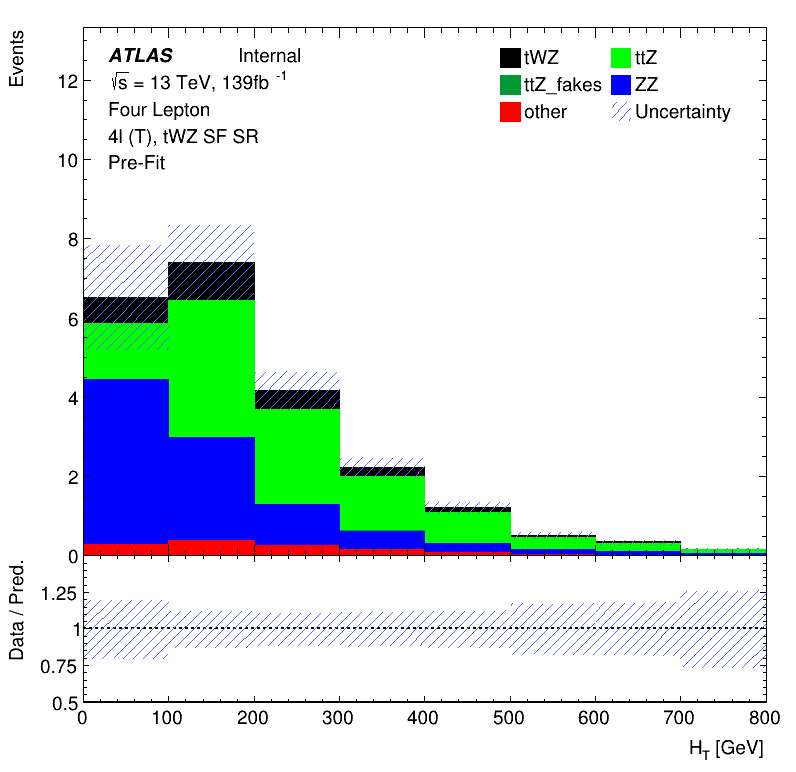
\includegraphics[width=.3\textwidth]{figures/PreFitPlots/lep4_tWZ_4T_SF_HT.png}   \quad
    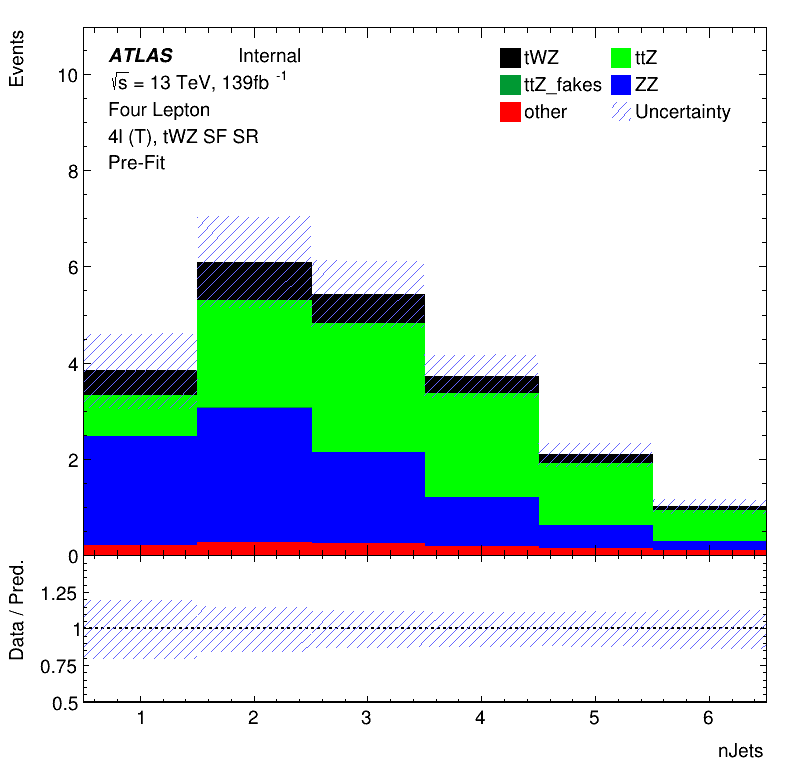
\includegraphics[width=.3\textwidth]{figures/PreFitPlots/lep4_tWZ_4T_SF_Num_Jets.png}

    \caption{\textbf{Top row:} MC predictions for $p_{T}$, $\eta$ and $\phi$ for next-to-next-to-leading (NNL) jets in the $tWZ$ SF SR region (\textit{blinded}) is shown. \textbf{Bottom row:} MC predictions for $H_{T}$ (scalar sum of Jet $p_{T}$) (left) and the Number of jets (right) in the $tWZ$ SF SR region (\textit{blinded}) is shown.}
    \label{fig:4lep-SF-SR-NNLjetPlots} 
\end{figure}



In Figure~\ref{fig:4lep-SF-SR-bjetPlots} MC predictions for $p_{T}$, $\eta$ and $\phi$ of the leading b-tagged jets, the scalar sum of b-tagged jet $p_{T}$ and the Number of b-tagged jets in the $tWZ$ SF SR region is shown.
\begin{figure}[htbp]
\centering
    %%%%%%%%%%%%%%%%%%
    %%%%% b jets %%%%%
    %%%%%%%%%%%%%%%%%%

    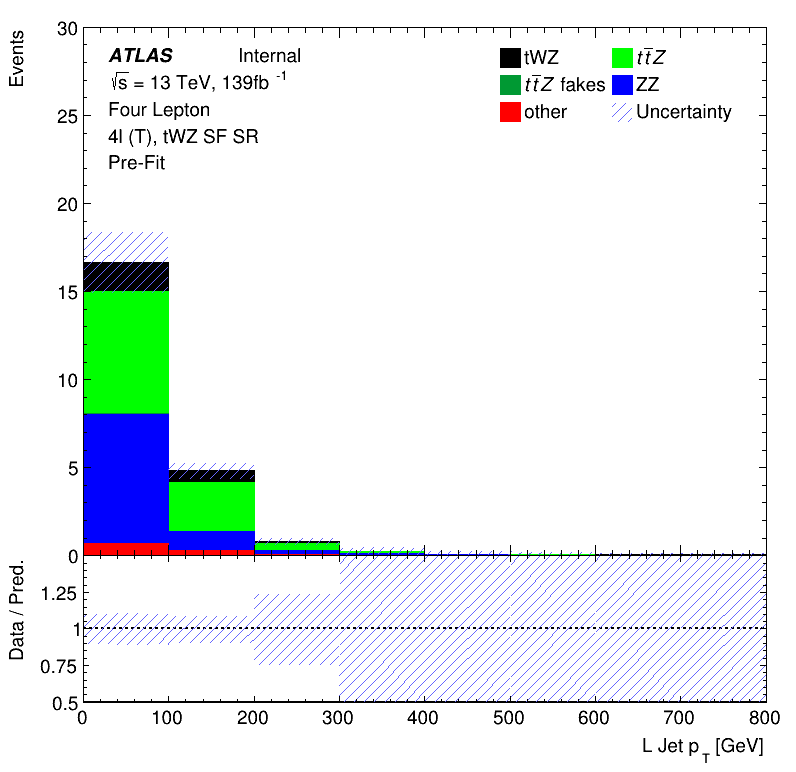
\includegraphics[width=.3\textwidth]{figures/PreFitPlots/lep4_tWZ_4T_SF_0_bJet_pt.png}   \quad
    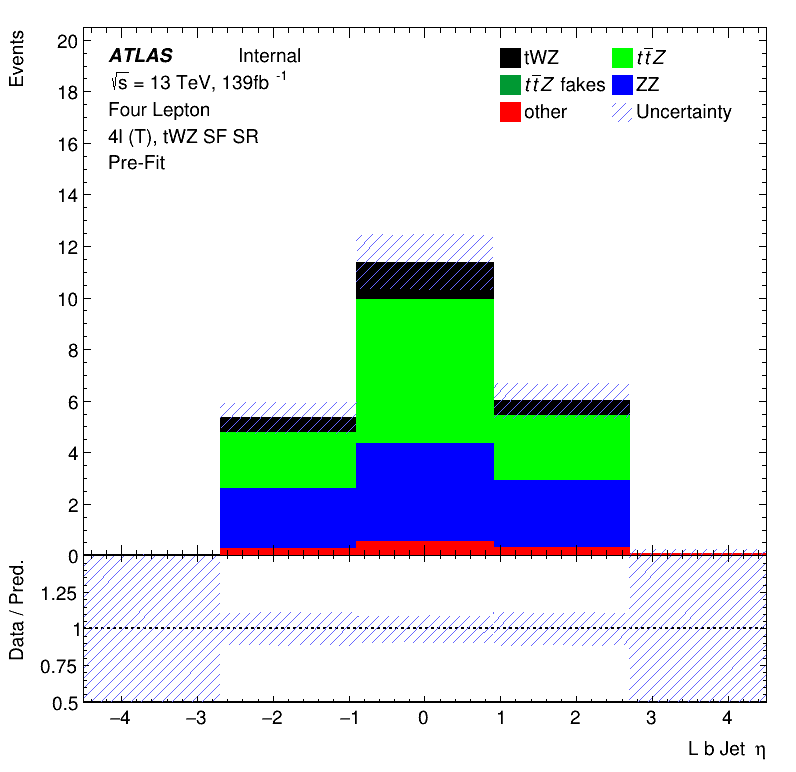
\includegraphics[width=.3\textwidth]{figures/PreFitPlots/lep4_tWZ_4T_SF_0_bJet_eta.png}    \quad
    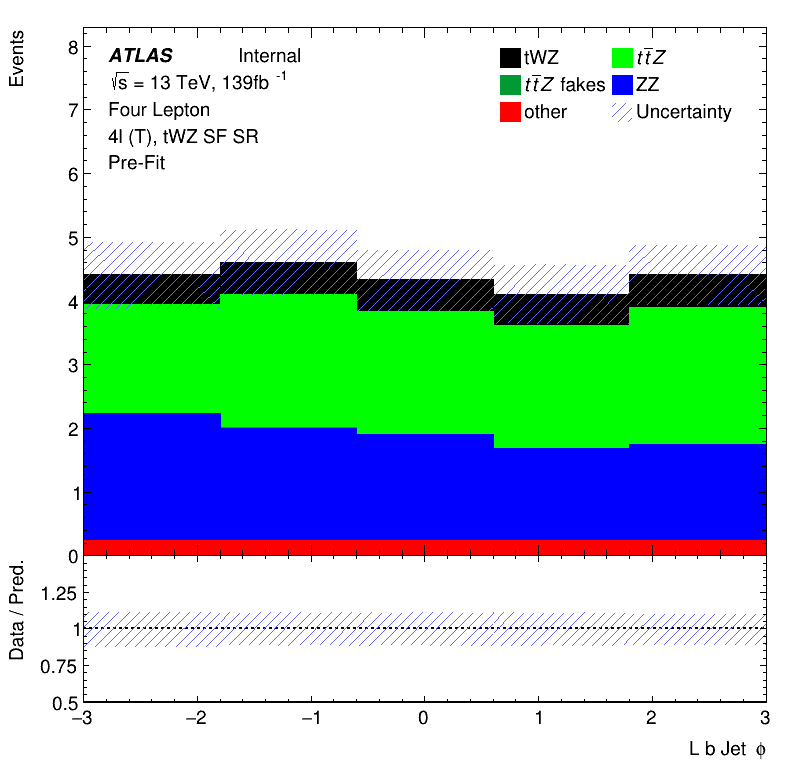
\includegraphics[width=.3\textwidth]{figures/PreFitPlots/lep4_tWZ_4T_SF_0_bJet_phi.png}

    \medskip

    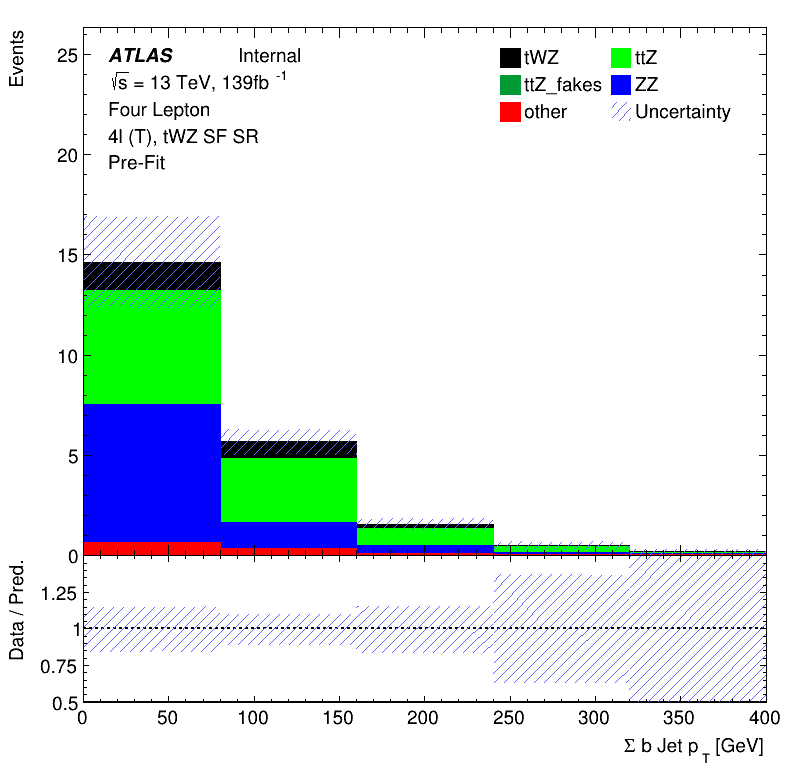
\includegraphics[width=.3\textwidth]{figures/PreFitPlots/lep4_tWZ_4T_SF_sum_bJet_Pt.png}  \quad
    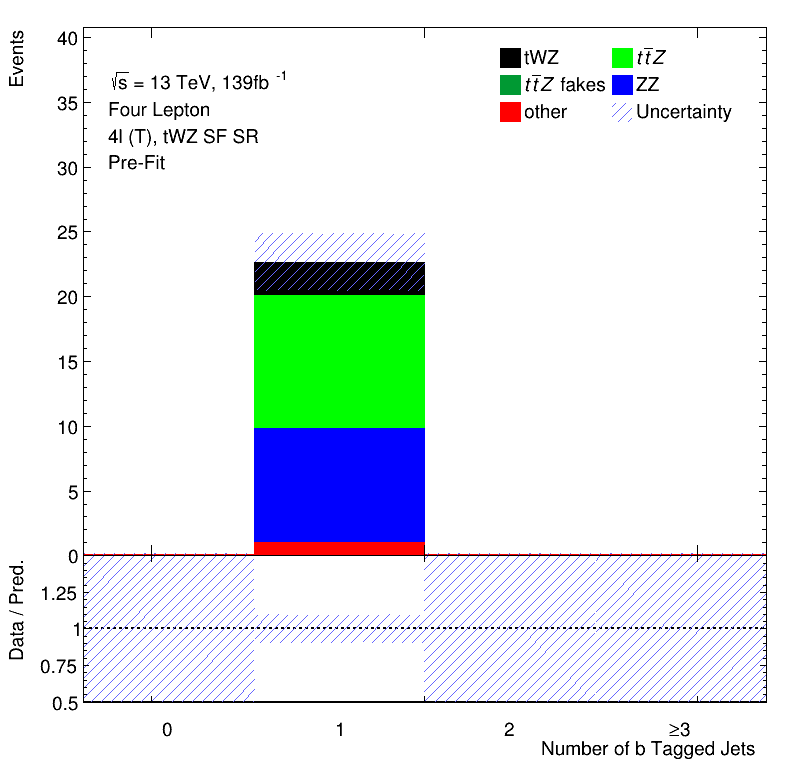
\includegraphics[width=.3\textwidth]{figures/PreFitPlots/lep4_tWZ_4T_SF_Num_bJets.png}

    \caption{\textbf{Top row:} MC predictions for $p_{T}$, $\eta$ and $\phi$ for leading b-tagged jets in the $tWZ$ SF SR region (\textit{blinded}) is shown. \textbf{Bottom row:} MC predictions for the scalar sum of b-tagged jet $p_{T}$ (left) and the Number of b-tagged jets (right) in the $tWZ$ SF SR region (\textit{blinded}) is shown.}
  \label{fig:4lep-SF-SR-bjetPlots}
\end{figure}

\subsection{$t\bar{t}Z$ CR}
\label{sec:controlplotstetralepton-ttZ-CR}

%%%%%%%%%%%%%%%%%%%%%%%%%%%%%%%%%%%%
%%%%%%%%%%%%%%%%%%%%%%%%%%%%%%%%%%%%
%%%%%%%      ttZ CR   %%%%%%%%%%
%%%%%%%%%%%%%%%%%%%%%%%%%%%%%%%%%%%%
%%%%%%%%%%%%%%%%%%%%%%%%%%%%%%%%%%%%

In this section, pre-fit distributions of variables in the $t\bar{t}Z$ CR are shown. More pre-fit distributions for the $t\bar{t}Z$ CR are shown in the appendix (Section \ref{sec:app-controlplotstetralepton-ttZ-CR}).\\\\

In Figure~\ref{fig:4lep-ttZ-CR-leptonPlots} MC predictions for $p_{T}$, $\eta$ and $\phi$ for leading (L) leptons and next-to-leading (NL) leptons in the $t\bar{t}Z$ CR region is shown.

\begin{figure}[htbp]
  \begin{tabular}{ccc}

    %%%%%%%%%%%%%%%
    %%% Leptons %%%
    %%%%%%%%%%%%%%%

    \includegraphics[width=.3\textwidth]{figures/PreFitPlots/lep4_ttZ_4T_L_lepton_pt.png} &
    \includegraphics[width=.3\textwidth]{figures/PreFitPlots/lep4_ttZ_4T_L_lepton_eta.png} &
    \includegraphics[width=.3\textwidth]{figures/PreFitPlots/lep4_ttZ_4T_L_lepton_phi.png} \\
    \includegraphics[width=.3\textwidth]{figures/PreFitPlots/lep4_ttZ_4T_NL_lepton_pt.png} &
    \includegraphics[width=.3\textwidth]{figures/PreFitPlots/lep4_ttZ_4T_NL_lepton_eta.png} &
    \includegraphics[width=.3\textwidth]{figures/PreFitPlots/lep4_ttZ_4T_NL_lepton_phi.png} \\

  \end{tabular}
    \caption{MC predictions for $p_{T}$, $\eta$ and $\phi$ for leading (L) leptons (top row) and next-to-leading (NL) leptons (bottom row) in the $t\bar{t}Z$ CR region (\textit{blinded}) is shown.}
  \label{fig:4lep-ttZ-CR-leptonPlots}
\end{figure}

In Figure~\ref{fig:4lep-ttZ-CR-LandNjetPlots} MC predictions for $p_{T}$, $\eta$ and $\phi$ for leading (L) jets and next-to-leading (NL) jets in the $t\bar{t}Z$ CR region is shown.

\begin{figure}[htbp]
  \begin{tabular}{ccc}
    %%%%%%%%%%%%%%%%%
    %%%%% jets %%%%%
    %%%%%%%%%%%%%%%%%

    \includegraphics[width=.3\textwidth]{figures/PreFitPlots/lep4_ttZ_4T_LJet_pt.png} &
    \includegraphics[width=.3\textwidth]{figures/PreFitPlots/lep4_ttZ_4T_LJet_eta.png} &
    \includegraphics[width=.3\textwidth]{figures/PreFitPlots/lep4_ttZ_4T_LJet_phi.png} \\
    \includegraphics[width=.3\textwidth]{figures/PreFitPlots/lep4_ttZ_4T_NLJet_pt.png} &
    \includegraphics[width=.3\textwidth]{figures/PreFitPlots/lep4_ttZ_4T_NLJet_eta.png} &
    \includegraphics[width=.3\textwidth]{figures/PreFitPlots/lep4_ttZ_4T_NLJet_phi.png} \\

  \end{tabular}
    \caption{MC predictions for $p_{T}$, $\eta$ and $\phi$ for leading (L) jets (top row) and next-to-leading (NL) jets (bottom row) in the $t\bar{t}Z$ CR region (\textit{blinded}) is shown.}
    \label{fig:4lep-ttZ-CR-LandNjetPlots} 
\end{figure}

In Figure~\ref{fig:4lep-ttZ-CR-NNLjetPlots} MC predictions for $p_{T}$, $\eta$ and $\phi$ of the next-to-next-to-leading (NNL) jets, $H_{T}$ (scalar sum of Jet $p_{T}$) and the Number of jets in the $t\bar{t}Z$ CR region is shown.


\begin{figure}[htbp]
 \centering

    %%%%%%%%%%%%%%%%%
    %%%%% jets %%%%%
    %%%%%%%%%%%%%%%%%

    \includegraphics[width=.3\textwidth]{figures/PreFitPlots/lep4_ttZ_4T_NNLJet_pt.png} \quad
    \includegraphics[width=.3\textwidth]{figures/PreFitPlots/lep4_ttZ_4T_NNLJet_eta.png} \quad
    \includegraphics[width=.3\textwidth]{figures/PreFitPlots/lep4_ttZ_4T_NNLJet_phi.png}

    \medskip

    \includegraphics[width=.3\textwidth]{figures/PreFitPlots/lep4_ttZ_4T_HT.png}   \quad
    \includegraphics[width=.3\textwidth]{figures/PreFitPlots/lep4_ttZ_4T_Num_Jets.png}

    \caption{\textbf{Top row:} MC predictions for $p_{T}$, $\eta$ and $\phi$ for next-to-next-to-leading (NNL) jets in the $t\bar{t}Z$ CR region (\textit{blinded}) is shown. \textbf{Bottom row:} MC predictions for $H_{T}$ (scalar sum of Jet $p_{T}$) (left) and the Number of jets (right) in the $t\bar{t}Z$ CR region (\textit{blinded}) is shown.}
    \label{fig:4lep-ttZ-CR-NNLjetPlots} 
\end{figure}



In Figure~\ref{fig:4lep-ttZ-CR-bjetPlots} MC predictions for $p_{T}$, $\eta$ and $\phi$ of the leading b-tagged jets, the scalar sum of b-tagged jet $p_{T}$ and the Number of b-tagged jets in the $t\bar{t}Z$ CR region is shown.
\begin{figure}[htbp]
\centering
    %%%%%%%%%%%%%%%%%%
    %%%%% b jets %%%%%
    %%%%%%%%%%%%%%%%%%

    \includegraphics[width=.3\textwidth]{figures/PreFitPlots/lep4_ttZ_4T_0_bJet_pt.png}   \quad
    \includegraphics[width=.3\textwidth]{figures/PreFitPlots/lep4_ttZ_4T_0_bJet_eta.png}    \quad
    \includegraphics[width=.3\textwidth]{figures/PreFitPlots/lep4_ttZ_4T_0_bJet_phi.png}

    \medskip

    \includegraphics[width=.3\textwidth]{figures/PreFitPlots/lep4_ttZ_4T_sum_bJet_Pt.png}  \quad
    \includegraphics[width=.3\textwidth]{figures/PreFitPlots/lep4_ttZ_4T_Num_bJets.png}

    \caption{\textbf{Top row:} MC predictions for $p_{T}$, $\eta$ and $\phi$ for leading b-tagged jets in the $t\bar{t}Z$ CR region (\textit{blinded}) is shown. \textbf{Bottom row:} MC predictions for the scalar sum of b-tagged jet $p_{T}$ (left) and the Number of b-tagged jets (right) in the $t\bar{t}Z$ CR region (\textit{blinded}) is shown.}
  \label{fig:4lep-ttZ-CR-bjetPlots}
\end{figure}




\subsection{$ZZb$ CR}
\label{sec:controlplotstetralepton-ZZb-CR}

%%%%%%%%%%%%%%%%%%%%%%%%%%%%%%%%%%%%
%%%%%%%%%%%%%%%%%%%%%%%%%%%%%%%%%%%%
%%%%%%%      ZZb CR   %%%%%%%%%%
%%%%%%%%%%%%%%%%%%%%%%%%%%%%%%%%%%%%
%%%%%%%%%%%%%%%%%%%%%%%%%%%%%%%%%%%%

In this section, pre-fit distributions of variables in the $ZZb$ CR are shown. More pre-fit distributions for the $ZZb$ CR are shown in the appendix (Section \ref{sec:app-controlplotstetralepton-ZZb-CR}).\\\\

In Figure~\ref{fig:4lep-ZZb-CR-leptonPlots} MC predictions for $p_{T}$, $\eta$ and $\phi$ for leading (L) leptons and next-to-leading (NL) leptons in the $ZZb$ CR region is shown.

\begin{figure}[htbp]
  \begin{tabular}{ccc}

    %%%%%%%%%%%%%%%
    %%% Leptons %%%
    %%%%%%%%%%%%%%%

    \includegraphics[width=.3\textwidth]{figures/PreFitPlots/lep4_ZZb_4T_L_lepton_pt.png} &
    \includegraphics[width=.3\textwidth]{figures/PreFitPlots/lep4_ZZb_4T_L_lepton_eta.png} &
    \includegraphics[width=.3\textwidth]{figures/PreFitPlots/lep4_ZZb_4T_L_lepton_phi.png} \\
    \includegraphics[width=.3\textwidth]{figures/PreFitPlots/lep4_ZZb_4T_NL_lepton_pt.png} &
    \includegraphics[width=.3\textwidth]{figures/PreFitPlots/lep4_ZZb_4T_NL_lepton_eta.png} &
    \includegraphics[width=.3\textwidth]{figures/PreFitPlots/lep4_ZZb_4T_NL_lepton_phi.png} \\

  \end{tabular}
    \caption{MC predictions for $p_{T}$, $\eta$ and $\phi$ for leading (L) leptons (top row) and next-to-leading (NL) leptons (bottom row) in the $ZZb$ CR region (\textit{blinded}) is shown.}
  \label{fig:4lep-ZZb-CR-leptonPlots}
\end{figure}

In Figure~\ref{fig:4lep-ZZb-CR-LandNjetPlots} MC predictions for $p_{T}$, $\eta$ and $\phi$ for leading (L) jets and next-to-leading (NL) jets in the $ZZb$ CR region is shown.

\begin{figure}[htbp]
  \begin{tabular}{ccc}
    %%%%%%%%%%%%%%%%%
    %%%%% jets %%%%%
    %%%%%%%%%%%%%%%%%

    \includegraphics[width=.3\textwidth]{figures/PreFitPlots/lep4_ZZb_4T_LJet_pt.png} &
    \includegraphics[width=.3\textwidth]{figures/PreFitPlots/lep4_ZZb_4T_LJet_eta.png} &
    \includegraphics[width=.3\textwidth]{figures/PreFitPlots/lep4_ZZb_4T_LJet_phi.png} \\
    \includegraphics[width=.3\textwidth]{figures/PreFitPlots/lep4_ZZb_4T_NLJet_pt.png} &
    \includegraphics[width=.3\textwidth]{figures/PreFitPlots/lep4_ZZb_4T_NLJet_eta.png} &
    \includegraphics[width=.3\textwidth]{figures/PreFitPlots/lep4_ZZb_4T_NLJet_phi.png} \\

  \end{tabular}
    \caption{MC predictions for $p_{T}$, $\eta$ and $\phi$ for leading (L) jets (top row) and next-to-leading (NL) jets (bottom row) in the $ZZb$ CR region (\textit{blinded}) is shown.}
    \label{fig:4lep-ZZb-CR-LandNjetPlots} 
\end{figure}

In Figure~\ref{fig:4lep-ZZb-CR-NNLjetPlots} MC predictions for $p_{T}$, $\eta$ and $\phi$ of the next-to-next-to-leading (NNL) jets, $H_{T}$ (scalar sum of Jet $p_{T}$) and the Number of jets in the $ZZb$ CR region is shown.


\begin{figure}[htbp]
 \centering

    %%%%%%%%%%%%%%%%%
    %%%%% jets %%%%%
    %%%%%%%%%%%%%%%%%

    \includegraphics[width=.3\textwidth]{figures/PreFitPlots/lep4_ZZb_4T_NNLJet_pt.png} \quad
    \includegraphics[width=.3\textwidth]{figures/PreFitPlots/lep4_ZZb_4T_NNLJet_eta.png} \quad
    \includegraphics[width=.3\textwidth]{figures/PreFitPlots/lep4_ZZb_4T_NNLJet_phi.png}

    \medskip

    \includegraphics[width=.3\textwidth]{figures/PreFitPlots/lep4_ZZb_4T_HT.png}   \quad
    \includegraphics[width=.3\textwidth]{figures/PreFitPlots/lep4_ZZb_4T_Num_Jets.png}

    \caption{\textbf{Top row:} MC predictions for $p_{T}$, $\eta$ and $\phi$ for next-to-next-to-leading (NNL) jets in the $ZZb$ CR region (\textit{blinded}) is shown. \textbf{Bottom row:} MC predictions for $H_{T}$ (scalar sum of Jet $p_{T}$) (left) and the Number of jets (right) in the $ZZb$ CR region (\textit{blinded}) is shown.}
    \label{fig:4lep-ZZb-CR-NNLjetPlots} 
\end{figure}



In Figure~\ref{fig:4lep-ZZb-CR-bjetPlots} MC predictions for $p_{T}$, $\eta$ and $\phi$ of the leading b-tagged jets, the scalar sum of b-tagged jet $p_{T}$ and the Number of b-tagged jets in the $ZZb$ CR region is shown.
\begin{figure}[htbp]
\centering
    %%%%%%%%%%%%%%%%%%
    %%%%% b jets %%%%%
    %%%%%%%%%%%%%%%%%%

    \includegraphics[width=.3\textwidth]{figures/PreFitPlots/lep4_ZZb_4T_bJet_pt.png}   \quad
    \includegraphics[width=.3\textwidth]{figures/PreFitPlots/lep4_ZZb_4T_0_bJet_eta.png}    \quad
    \includegraphics[width=.3\textwidth]{figures/PreFitPlots/lep4_ZZb_4T_0_bJet_phi.png}

    \medskip

    \includegraphics[width=.3\textwidth]{figures/PreFitPlots/lep4_ZZb_4T_sum_bJet_Pt.png}  \quad
    \includegraphics[width=.3\textwidth]{figures/PreFitPlots/lep4_ZZb_4T_Num_bJets.png}

    \caption{\textbf{Top row:} MC predictions for $p_{T}$, $\eta$ and $\phi$ for leading b-tagged jets in the $ZZb$ CR region (\textit{blinded}) is shown. \textbf{Bottom row:} MC predictions for the scalar sum of b-tagged jet $p_{T}$ (left) and the Number of b-tagged jets (right) in the $ZZb$ CR region (\textit{blinded}) is shown.}
  \label{fig:4lep-ZZb-CR-bjetPlots}
\end{figure}



\subsection{$(tWZ)_{\text{fake}}$ CR}
\label{sec:controlplotstetralepton-tWZ-fake-CR}

%%%%%%%%%%%%%%%%%%%%%%%%%%%%%%%%%%%%
%%%%%%%%%%%%%%%%%%%%%%%%%%%%%%%%%%%%
%%%%%%%      ZZb CR   %%%%%%%%%%
%%%%%%%%%%%%%%%%%%%%%%%%%%%%%%%%%%%%
%%%%%%%%%%%%%%%%%%%%%%%%%%%%%%%%%%%%

In this section, pre-fit distributions of variables in the $(tWZ)_{\text{fake}}$ CR are shown. More pre-fit distributions for the $(tWZ)_{\text{fake}}$ CR are shown in the appendix (Section \ref{sec:app-controlplotstetralepton-tWZ-fake-CR}).\\\\

In Figure~\ref{fig:4lep-tWZ-fake-CR-leptonPlots} MC predictions for $p_{T}$, $\eta$ and $\phi$ for leading (L) leptons and next-to-leading (NL) leptons in the $(tWZ)_{\text{fake}}$ CR region is shown.

\begin{figure}[htbp]
  \begin{tabular}{ccc}

    %%%%%%%%%%%%%%%
    %%% Leptons %%%
    %%%%%%%%%%%%%%%

    \includegraphics[width=.3\textwidth]{figures/PreFitPlots/lep4_tWZ_3T1L_L_lepton_pt.png} &
    \includegraphics[width=.3\textwidth]{figures/PreFitPlots/lep4_tWZ_3T1L_L_lepton_eta.png} &
    \includegraphics[width=.3\textwidth]{figures/PreFitPlots/lep4_tWZ_3T1L_L_lepton_phi.png} \\
    \includegraphics[width=.3\textwidth]{figures/PreFitPlots/lep4_tWZ_3T1L_NL_lepton_pt.png} &
    \includegraphics[width=.3\textwidth]{figures/PreFitPlots/lep4_tWZ_3T1L_NL_lepton_eta.png} &
    \includegraphics[width=.3\textwidth]{figures/PreFitPlots/lep4_tWZ_3T1L_NL_lepton_phi.png} \\

  \end{tabular}
    \caption{MC predictions for $p_{T}$, $\eta$ and $\phi$ for leading (L) leptons (top row) and next-to-leading (NL) leptons (bottom row) in the $(tWZ)_{\text{fake}}$ CR region (\textit{blinded}) is shown.}
  \label{fig:4lep-tWZ-fake-CR-leptonPlots}
\end{figure}

In Figure~\ref{fig:4lep-tWZ-fake-CR-LandNjetPlots} MC predictions for $p_{T}$, $\eta$ and $\phi$ for leading (L) jets and next-to-leading (NL) jets in the $(tWZ)_{\text{fake}}$ CR region is shown.

\begin{figure}[htbp]
  \begin{tabular}{ccc}
    %%%%%%%%%%%%%%%%%
    %%%%% jets %%%%%
    %%%%%%%%%%%%%%%%%

    \includegraphics[width=.3\textwidth]{figures/PreFitPlots/lep4_tWZ_3T1L_LJet_pt.png} &
    \includegraphics[width=.3\textwidth]{figures/PreFitPlots/lep4_tWZ_3T1L_LJet_eta.png} &
    \includegraphics[width=.3\textwidth]{figures/PreFitPlots/lep4_tWZ_3T1L_LJet_phi.png} \\
    \includegraphics[width=.3\textwidth]{figures/PreFitPlots/lep4_tWZ_3T1L_NLJet_pt.png} &
    \includegraphics[width=.3\textwidth]{figures/PreFitPlots/lep4_tWZ_3T1L_NLJet_eta.png} &
    \includegraphics[width=.3\textwidth]{figures/PreFitPlots/lep4_tWZ_3T1L_NLJet_phi.png} \\

  \end{tabular}
    \caption{MC predictions for $p_{T}$, $\eta$ and $\phi$ for leading (L) jets (top row) and next-to-leading (NL) jets (bottom row) in the $(tWZ)_{\text{fake}}$ CR region (\textit{blinded}) is shown.}
    \label{fig:4lep-tWZ-fake-CR-LandNjetPlots} 
\end{figure}

In Figure~\ref{fig:4lep-tWZ-fake-CR-NNLjetPlots} MC predictions for $p_{T}$, $\eta$ and $\phi$ of the next-to-next-to-leading (NNL) jets, $H_{T}$ (scalar sum of Jet $p_{T}$) and the Number of jets in the $(tWZ)_{\text{fake}}$ CR region is shown.


\begin{figure}[htbp]
 \centering

    %%%%%%%%%%%%%%%%%
    %%%%% jets %%%%%
    %%%%%%%%%%%%%%%%%

    \includegraphics[width=.3\textwidth]{figures/PreFitPlots/lep4_tWZ_3T1L_NNLJet_pt.png} \quad
    \includegraphics[width=.3\textwidth]{figures/PreFitPlots/lep4_tWZ_3T1L_NNLJet_eta.png} \quad
    \includegraphics[width=.3\textwidth]{figures/PreFitPlots/lep4_tWZ_3T1L_NNLJet_phi.png}

    \medskip

    \includegraphics[width=.3\textwidth]{figures/PreFitPlots/lep4_tWZ_3T1L_HT.png}   \quad
    \includegraphics[width=.3\textwidth]{figures/PreFitPlots/lep4_tWZ_3T1L_Num_Jets.png}

    \caption{\textbf{Top row:} MC predictions for $p_{T}$, $\eta$ and $\phi$ for next-to-next-to-leading (NNL) jets in the $(tWZ)_{\text{fake}}$ CR region (\textit{blinded}) is shown. \textbf{Bottom row:} MC predictions for $H_{T}$ (scalar sum of Jet $p_{T}$) (left) and the Number of jets (right) in the $(tWZ)_{\text{fake}}$ CR region (\textit{blinded}) is shown.}
    \label{fig:4lep-tWZ-fake-CR-NNLjetPlots} 
\end{figure}



In Figure~\ref{fig:4lep-tWZ-fake-CR-bjetPlots} MC predictions for $p_{T}$, $\eta$ and $\phi$ of the leading b-tagged jets, the scalar sum of b-tagged jet $p_{T}$ and the Number of b-tagged jets in the $(tWZ)_{\text{fake}}$ CR region is shown.
\begin{figure}[htbp]
\centering
    %%%%%%%%%%%%%%%%%%
    %%%%% b jets %%%%%
    %%%%%%%%%%%%%%%%%%

    \includegraphics[width=.3\textwidth]{figures/PreFitPlots/lep4_tWZ_3T1L_0_bJet_pt.png}   \quad
    \includegraphics[width=.3\textwidth]{figures/PreFitPlots/lep4_tWZ_3T1L_0_bJet_eta.png}    \quad
    \includegraphics[width=.3\textwidth]{figures/PreFitPlots/lep4_tWZ_3T1L_0_bJet_phi.png}

    \medskip

    \includegraphics[width=.3\textwidth]{figures/PreFitPlots/lep4_tWZ_3T1L_sum_bJet_Pt.png}  \quad
    \includegraphics[width=.3\textwidth]{figures/PreFitPlots/lep4_tWZ_3T1L_Num_bJets.png}

    \caption{\textbf{Top row:} MC predictions for $p_{T}$, $\eta$ and $\phi$ for leading b-tagged jets in the $(tWZ)_{\text{fake}}$ CR region (\textit{blinded}) is shown. \textbf{Bottom row:} MC predictions for the scalar sum of b-tagged jet $p_{T}$ (left) and the Number of b-tagged jets (right) in the $(tWZ)_{\text{fake}}$ CR region (\textit{blinded}) is shown.}
  \label{fig:4lep-tWZ-fake-CR-bjetPlots}
\end{figure}


Given the limited statistics which we are presented with in the tetralepton channel, we nevertheless observe relatively good agreement overall between data and MC.

\section{Fake Lepton Estimation}
\label{sec:fakelepest}
Fake leptons are objects reconstructed as leptons, but do not correspond to the leptons which we are interested in our analysis. Fake leptons can be split up into two main categories, irreducible (prompt) fakes and reducible (non-prompt) fakes. Irreducible fakes are true leptons which do not come from the process of interest. Reducible fakes are objects which are mis-identified or incorrectly reconstructed as leptons. In the ATLAS detector, the probability for a fake to occur is very low.\\\\

We aim to estimate the fake lepton contribution in this analysis. We start off by noticing that \ttZ is our most dominant background ($\sim$ 75$\%$ of the total background contribution) and will therefore have the largest fake component compared to all other samples considered in the analysis. The fake lepton efficiency, $\epsilon$, can be written as $\epsilon = \frac{N_{\text{fake}}^{\text{tight}}}{N_{\text{fake}}^{\text{loose}}}$, where $N_{\text{fake}}^{\text{tight}}$ is the number of fake leptons which pass the tight lepton selection (See Section~\ref{sec:lepton-object}) and $N_{\text{fake}}^{\text{loose}}$ is the number of fake leptons which pass the loose lepton selection (See Section~\ref{sec:lepton-object}). The probability of one fake lepton to occur, $P(\text{one fake }\ell)$, is proportional to $\epsilon$ and the probability for two fakes to occur is simply, $P(\text{two fake }\ell) = (P(\text{one fake }\ell))^{2} \propto \epsilon^{2}$. Since $\epsilon < 1$, we have $P(\text{one fake }\ell) \ll P(\text{two fake }\ell)$. For the purposes of this analysis we shall investigate the fake lepton component to first order and therefore will only consider the case where one fake lepton occurs in a \ttZ event.\\\\

Firstly, we split up the dominant \ttZ background into \ttZ and $(t\bar{t}Z)_{\text{fake}}$ components. Secondly, we define a $(tWZ)_{\text{fake}}$ CR (See Section~\ref{sec:regionsAndEventSelection}) which is enhanced in fakes and aims to constrain the $(t\bar{t}Z)_{\text{fake}}$ background in the SR.

 All events which contribute to the $(t\bar{t}Z)_{\text{fake}}$ background are determined by the \texttt{IFF Truth Classifier}~\cite{IFFTruthClassifier}. The \texttt{IFF Truth Classifier} is a tool which aims to classify leptons based off their truth information. It uses the more general \texttt{MCTruthClassifier}~\cite{MCTruthClassifier} tool's output as input and returns one of the following lepton categories: \texttt{Unknown}, \texttt{KnownUnknown} (leptons which can (in priciple) be classified, but the \texttt{MCTruthClassifier} fails to classify the lepton's truth type or origin), \texttt{IsoElectron}, \texttt{ChargeFlipIsoElectron}, \texttt{PromptMuon}, \texttt{PromptPhotonConversion}, \texttt{ElectronFromMuon}, \texttt{TauDecay}, \texttt{BHadronDecay}, \texttt{CHadronDecay} or \texttt{LightFlavorDecay} (More details~\cite{IFFTruthClassifier-leptonCategories}). Given these categories, we consider leptons classified as \texttt{PromptPhotonConversion}, \texttt{BHadronDecay}, \texttt{CHadronDecay} or \texttt{LightFlavorDecay} (i.e. a lepton originating from the decay of a $b$-Hadron, $c$-Hadron or light-flavour jet) to be fakes. Since we only consider events with one fake lepton to contribute to our $(t\bar{t}Z)_{\text{fake}}$ background, we require that events which contribute to this background are those where exactly one lepton from the \ttZ sample are classified by the \texttt{IFF Truth Classifier} with one of the three aforementioned categories.

The $(tWZ)_{\text{fake}}$ CR aims to be as similar as possible to the $tWZ$ SRs, but enhanced in fakes. This CR can then be used to constrain the normalisation of the $(t\bar{t}Z)_{\text{fake}}$ template from data, since we use the \textit{mixed data and MC fit} (See Section \ref{sec:pipelineAnalysis-and-TRF}) which uses the data in the CRs to construct a modified ASIMOV dataset from the fitted nuisance parameters from a background only fit to the CRs. To ensure that this region is enhanced in fakes, we require that it contains 3 tight leptons and 1 loose lepton, since loose leptons are more likely to be fakes. By using the $p_{T}$ of the loose lepton ($p_{T}(\text{Loose Lepton})$) in this region as the variable used in the fit, the shape (and normalisation) of the $(t\bar{t}Z)_{\text{fake}}$ template can be constrained.

The proportion of fake events in a region can be calculated by taking the ratio of the $(t\bar{t}Z)_{\text{fake}}$ MC yield in the region and the total MC yield in the region. These are 0.0035 $\pm$ 0.0025, 0.0014 $\pm$ 0.0012 and 0.10 $\pm$ 0.051 for the $tWZ$ OF SR, $tWZ$ SF SR and $(tWZ)_{\text{fake}}$ CR respectively. This shows that there is significantly more $(t\bar{t}Z)_{\text{fake}}$ events in the $(tWZ)_{\text{fake}}$ CR compared to the $tWZ$ SRs, therefore justifying our inclusion of the $(tWZ)_{\text{fake}}$ CR in the fit (to constrain the $(t\bar{t}Z)_{\text{fake}}$ background).

\section{Machine Learning Techniques}
Now that we have our baseline selections applied and our regions defined, we implement two Boosted Decision Trees (BDT) in order to discriminate between \tWZ and our most prominent background process, \ttZ and \ZZ. We chose to use a BDT, as opposed to another ML algorithm, since they are very stable and perform well with minimal/no optimisation or tweaking of the hyper parameters. A multi-layered sequential neutral network was tried, however, it was out-performed by a BDT. More specifically, Scikit-Learn's \texttt{GradientBoostingClassifier} was used.\\\\
Two different BDTs were used, the first aims to discriminate between \tWZ events and its major backgrounds, \ttZ and \ZZ. The second aims to discriminate between $\ell b$ systems which originate from the decay of a top quark ($t\rightarrow W(\rightarrow \ell \nu) b$) and those which do not. We refer to these two BDTs as an \texttt{event-level} and an \texttt{object-level} classifier respectively. The discriminator output from the object-level BDT can be converted to a variable which can then be used as input to the event-level BDT.
\subsection{Object-level BDT}
\label{sec:object-level-bdt}
The object-level BDT was trained on a $t\bar{t}$ sample, using the same jet and lepton baseline selections as outlined in Table \ref{tab:4Lep-cutsummary}. Minor differences occur between this $t\bar{t}$ sample and the MC samples used for the rest of the analysis, such as the use of the older MV2c10 $b$-tagger. This is such since the $t\bar{t}$ sample was used in a separate analysis and was re-purposed for this analysis. Despite these differences, the trained object-level BDT is sufficient in this case, since we expect that $\ell b$ systems present in the $t\bar{t}$ sample are similar enough to those present in the MC samples used in the rest of the analysis. Additionally, we opted to use this disjoint $t\bar{t}$ sample as to avoid resorting to use our MC samples used in the rest of the analysis which is heavily limited on statistics, therefore maximizing the amount of MC statistics used in the fitting procedure and the training of the event-level BDT.\\\\

The signal class is defined to consist of reconstructed $\ell b$ systems (defined as the sum of the 4-vectors of the lepton and $b$-jet) coming from top quarks which are well matched to their truth counterparts. In particular, we require that $\Delta R$ between the reconstructed and truth $\ell b$ system is less than 0.05. We additionally require that the reconstructed lepton and the truth top have charges with the same sign (since $t\rightarrow b\ell^{+}\bar{\nu_{\ell}}$ and $\bar{t}\rightarrow \bar{b}\ell^{-}\nu_{\ell}$). Conversely, the background class is defined to consist of reconstructed $\ell b$ systems which are not well matched to their truth counterparts. In particular, we require that $\Delta R$ between the reconstructed and truth $\ell b$ system is greater than 0.05. We additionally require that the reconstructed lepton and the truth top have charges with opposite sign. These definitions for the signal and background classes ensure that the signal class consists of mostly $\ell b$ systems originating from tops and the background class consists of mostly $\ell b$ systems which do not originate from a top decay.\\\\

Different observables corresponding to an $\ell b$ system were used as input to training. The optimum values for the hyper-parameters used were determined by training the BDT with a range of different values for the hyper-parameters and choosing the set of values which maximized the mean accuracy (based off 5 fold kfold cross-validation). This method is more commonly referred to as hyper-parameter optimisation or tuning. After hyperparameter optimisation, the mean accuracy of each fold increased from 0.76 to 0.77 ($\sim 1\%$ increase).

In Table~\ref{tab:object-bdt-variables}, the variables used in training the object-level BDT are shown.
\begin{table}[htbp!]
\captionsetup{width=0.6\textwidth}
\centering
	\resizebox{0.6\textwidth}{!}{%
	\begin{tabular}{c|c}
\toprule
	Observable	& Description   \\
	\hline
    $m(\ell b)$ & Invariant mass of the $\ell b$ system \\
     $p_{T}(\ell b)$ & $p_{T}$ of the $\ell b$ system \\
    $\Delta \eta (\ell,b)$ & $\Delta \eta$ between the $\ell$ and $b$-tagged jet \\
   $\Delta \phi (\ell, b)$ & $\Delta \phi$ between the $\ell$ and $b$-tagged jet \\
    $\Delta R (\ell, b)$ & $\Delta R$ between the $\ell$ and $b$-tagged jet \\
    
\bottomrule
	\end{tabular}}
\caption{A list of the observables used in the object-level BDT, ordered by importance (descending, top to bottom) is shown.}

	\label{tab:object-bdt-variables}
\end{table}



In Figure~\ref{fig:norm-object-bdt-vars}, normalised distributions of the signal and background classes for the training set of all variables used in the object-level BDT are show.


\begin{figure}
    \centering

    
    \includegraphics[width=.3\textwidth]{figures/bdtPlots/normPlot_m_lb.png} 
    \includegraphics[width=.3\textwidth]{figures/bdtPlots/normPlot_pt_lb.png} 
    \includegraphics[width=.3\textwidth]{figures/bdtPlots/normPlot_delEta_lb.png} 
    \includegraphics[width=.3\textwidth]{figures/bdtPlots/normPlot_delPhi_lb.png} 
    \includegraphics[width=.3\textwidth]{figures/bdtPlots/normPlot_delR_lb.png} 
    
    \caption{Normalised distributions of the signal and background classes for the training set of all variables used in the object-level BDT (ordered from top left to bottom right via decreasing importance) are shown. The red and blue dotted lined histograms represent the signal and background classes events (normalised to an area of 1), respectively. The variable used in training is shown on the x-axis. The y-axis shows the relative number of events for the signal and background classes (in arbitrary units). \textbf{From top left to bottom right:} Invariant mass of the $\ell b$ system. The $p_{T}$ of the $\ell b$ system. $\Delta \eta$ between the $\ell$ and $b$-tagged jet. $\Delta \phi$ between the $\ell$ and $b$-tagged jet. $\Delta R$ between the $\ell$ and $b$-tagged jet. }
    \label{fig:norm-object-bdt-vars}
\end{figure}

Overall the BDT input variables show a large amount of discrimination.

In Table~\ref{tab:object-bdt-hyperParams}, the hyper-parameters used in the object-level BDT is shown.
\begin{table}[htbp!]
\large
	\resizebox{1\textwidth}{!}{%
		\begin{tabular}{c|c|c}
			\toprule
			Hyper-parameter &Value & Description\\
			\hline
			\texttt{loss} & \texttt{deviance} & The loss function to be optimised\\
			\texttt{criterion} &\texttt{friedman$\_$mse} & The function used to measure the quality of a split\\
			\texttt{n$\_$estimators} &\texttt{200} & The number of boosting stages to perform\\
			\texttt{learning$\_$rate} & \texttt{0.1}& The step size at each iteration during optimisation\\
			\texttt{max$\_$depth} & \texttt{6}& The maximum depth of the individual regression estimators\\
			\texttt{min$\_$samples$\_$split} & \texttt{2} & The minimum number of samples (events) required to split an internal node\\
			\texttt{min$\_$samples$\_$leaf} & \texttt{1} & The minimum number of samples (events) required to be at a leaf node\\
			\texttt{validation$\_$fraction} & \texttt{0.1}& The proportion of training data to set aside as validation set for early stopping\\
			\texttt{n$\_$iter$\_$no$\_$change} & \texttt{20} & Training terminates when the validation score (determined by the validation set) does not improve in all of the previous\\ 
			
			\bottomrule
			
		\end{tabular}}
		\caption{A list of the hyper-parameters used in the object-level BDT is shown. Hyperparameters not listed in this table use the default values as stated in the Scikit-learn Documentation\cite{skLearnGBClassifierDocs}.}
	\label{tab:object-bdt-hyperParams}
\end{table}

The number of events used in training for the signal and background classes were 347952 and 266636 respectively. Imbalanced datasets can cause ML classifiers to ignore small classes while concentrating on classifying large classes more accurately, which may result in the trained classifier performing sub-optimally. In order to correct this dataset imbalance, we ensure that the relative weighting of each event is such that the sum of the signal weights is equal to the sum of the background weights.
In Figure~\ref{fig:object-bdt-overtrain-check} the normalised histograms of the training and test sets (extracted from fold 5 from a 5 fold kfold cross validation) for signal and background is shown.


\begin{figure}[h!]
	\includegraphics[scale=0.8]{figures/overtrainingCheck_4lep_lb.png}
	\centering
	\caption{Normalised histograms of the object-level BDT discriminator output from the signal and background classes for the training and test sets from the 5th fold in a 5 fold kfold cross validation is shown. The output of the object-level BDT is shown on the x-axis and the relative number of events (in arbitrary units) is shown on the y-axis. The training set for the signal class is shown by the red dotted histogram. The test set for the signal class is shown by the red points, with the total uncertainty represented by the vertical error bars. The training set for the background class is shown by the blue dotted histogram. The test set for the background class is shown by the blue points, with the total uncertainty represented by the vertical error bars.}
	\label{fig:object-bdt-overtrain-check}
\end{figure}

We can see that the shapes of the training and test sets for both signal and background are very similar. This is a good indicator that no over-training occurred. Another over-training check is performed using 5 fold kfold cross validation. We ensure that the variance of the mean accuracy of each folds' test set in cross validation is substantially small. This indicates that fluctuations in features from different training sets are not learnt by the classifier. For the object-level classifier, a variance of 3.24$\times 10^{-7}$ was calculated for the mean accuracies of each folds' test set in cross validation, providing further evidence that no over-training occurred. \\\\

The output from the object-level BDT was used to construct a variable to be used as input to the event-level BDT. The event-level BDT aims to discriminate between \tWZ and our most prominent background, $t\bar{t}Z$. We therefore aim to construct a variable from the output of the object-level BDT which discriminates well between \tWZ and \ttZ. Since \tWZ events contain one top quark and \ttZ events contain two top quarks, we expect that \tWZ events have one $\ell b$ combination which scores well and we expect that \ttZ events have two $\ell b$ combinations which score well. We construct a variable, BDTScore$(\frac{\text{Best}}{\text{2nd Best}})$, which takes the ratio of the scores of the top scoring $\ell b$ system to the 2nd best scoring $\ell b$ system. We expect this variable to be large for \tWZ events and closer to one for \ttZ events, therefore providing discrimination between \tWZ and \ttZ.\\\\

In Figure~\ref{fig:bdtscore-bestover2ndbest}, normalised distributions of the signal and total background of the BDTScore$(\frac{\text{Best}}{\text{2nd Best}})$ variable in the $tWZ$ OF SR, $tWZ$ SF SR and $t\bar{t}Z$ CR are shown.
\begin{figure}
    \centering
    \includegraphics[width=0.3\textwidth]{figures/bdtPlots/lep4_tWZ_4T_OF_bdtScorebest.png}
    \includegraphics[width=0.3\textwidth]{figures/bdtPlots/lep4_tWZ_4T_SF_bdtScorebest.png}
    \includegraphics[width=0.3\textwidth]{figures/bdtPlots/lep4_ttZ_4T_bdtScorebest.png}
    \caption{Normalised distributions of the signal and total background of the BDTScore$(\frac{\text{Best}}{\text{2nd Best}})$ variable in the $tWZ$ OF SR, $tWZ$ SF SR and $t\bar{t}Z$ CR are shown (left to right). The dotted red and solid blue lines represent the distributions (normalised to an area of 1) of the signal and total background events respectively. The x-axis shows the BDTScore$(\frac{\text{Best}}{\text{2nd Best}})$ and the y-axis show the relative number of events (in arbitrary units).}
    \label{fig:bdtscore-bestover2ndbest}
\end{figure}

There doesn't seem to be a large amount of discrimination between signal and background for BDTScore$(\frac{\text{Best}}{\text{2nd Best}})$ in either of the above regions. We do however see some discrimination in bins near a value of 1, where the number of background events exceed the number of signal events, which is what we expect. This effect is slightly more exaggerated in the $t\bar{t}Z$ CR than the $tWZ$ SRs. This can be explained since we expect to have a larger proportion of $t\bar{t}Z$ events (events with two $\ell b$ systems) in the $t\bar{t}Z$ CR. Despite the apparent lack of discrimination between signal and background events from this variable, when used as input to training in the event-level BDT (see Section~\ref{sec:event-level-bdt}), it ranks relatively high on variable importance (see Table~\ref{tab:event-bdt-variables}) and thus improves the mean accuracy of the classifier. The tells us that the event-level BDT is taking advantage of the discrimination between signal and background present in the BDTScore$(\frac{\text{Best}}{\text{2nd Best}})$ variable.

\subsection{Event-level BDT}
\label{sec:event-level-bdt}
The event-level BDT was trained on 50$\%$ of the \tWZ MC sample's events for the signal class and similarly, 50$\%$ of the \ttZ and $ZZ$ MC sample's events were used for the background class. The samples we train on are individual events, with the features being carefully chosen observables. These observables are chosen on the basis that they are somewhat uncorrelated from one another and show a relatively large amount of separation power between \tWZ and \ttZ. Similarly to the object-level BDT, the optimum values for the hyper-parameters used were determined via hyper-parameter optimisation.  After hyperparameter optimisation, the mean accuracy of each fold (determined from 5 fold kfold cross validation) increased from 0.72 to 0.74 ($\sim 3\%$ increase). 

In Table~\ref{tab:event-bdt-variables}, the variables used in training the event-level BDT are shown.
\begin{table}[htbp!]

	\resizebox{\textwidth}{!}{%
	\begin{tabular}{c|c}
    \toprule
	Observable	& Description   \\
	\hline
	2$\nu$SM	& Maximum weight from the 2$\nu$SM algorithm \\
	$HT$	&  Scalar sum of jet $p_{T}$  \\
    $LT$ & Scalar sum of lepton $p_{T}$\\
	$\sum p_{T}(b-jet)$	& Scalar sum of $b$-tagged jet $p_{T}$  \\
	BDTScore$(\frac{\text{Best}}{\text{2nd Best}})$ & Ratio of the top scoring $\ell b$ system to the 2nd best scoring $\ell b$ system from the output of the object-level BDT ($\ell b$ classifier)\\
		 $\Delta \eta (\ell_{1,Non-Z}, \ell_{2,Non-Z})$ & $\Delta \eta$ between the two leptons, not coming from a $Z$ candidate\\
		 $min(m(\ell b))$ & Mass of the $\ell b$ system with the smallest mass \\
	 $\Delta \phi (\ell_{1,Non-Z} \ell_{2,Non-Z}, b_{1})$ & $\Delta \phi$ between the non-$Z$ lepton system (leptons not originating from a $Z$-candiate) and the leading $b$-tagged jet\\

    \bottomrule
\end{tabular}}
\caption{A list of the observables used in the event-level BDT, ordered by importance (descending, top to bottom) is shown.}
	\label{tab:event-bdt-variables}
\end{table}

In Figure~\ref{fig:norm-event-bdt-vars}, normalised distributions of the signal and background classes for the training set of all variables used in the event-level BDT are show.


\begin{figure}
    \centering

    
    \includegraphics[width=.3\textwidth]{figures/bdtPlots/normPlot_max_2vSM_weight.png} 
    \includegraphics[width=.3\textwidth]{figures/bdtPlots/normPlot_HT.png} 
    \includegraphics[width=.3\textwidth]{figures/bdtPlots/normPlot_LT.png} 
    \includegraphics[width=.3\textwidth]{figures/bdtPlots/normPlot_sum_bJet_pt.png} 
    \includegraphics[width=.3\textwidth]{figures/bdtPlots/normPlot_BDT_Score_bestOver2ndBest.png} 
    \includegraphics[width=.3\textwidth]{figures/bdtPlots/normPlot_delEta_lNonZ_lNonZ.png} 
    \includegraphics[width=.3\textwidth]{figures/bdtPlots/normPlot_lb_min_m.png} 
    \includegraphics[width=.3\textwidth]{figures/bdtPlots/normPlot_delPhi_llNonZ_b0.png} 
    
    \caption{Normalised distributions of the signal and background classes for the training set of all variables used in the event-level BDT (ordered from top left to bottom right via decreasing importance) are shown. The red and blue dotted lined histograms represent the signal and background classes events (normalised to an area of 1), respectively. The variable used in training is shown on the x-axis. The y-axis shows the relative number of events for the signal and background classes (in arbitrary units). \textbf{From top left to bottom right:} Output weight from the 2$\nu$SM algorithm (See Section~\ref{sec:2vsm}). Scalar sum of jet $p_{T}$. Scalar sum of lepton $p_{T}$. Sum of $b$-tagged jet $p_{T}$. Output from the object-level BDT (See Section~\ref{sec:object-level-bdt}). $\Delta \eta$ between the two leptons, not coming from a $Z$ candidate. Mass of the $\ell b$ system with the smallest mass. $\Delta \phi$ between the non-$Z$ lepton system (leptons not originating from a $Z$-candidate) and the leading $b$-tagged jet.}
    \label{fig:norm-event-bdt-vars}
\end{figure}

Overall the BDT input variables show a reasonable amount of discrimination. In particular the output weight from the 2$\nu$SM algorithm shows the most discrimination. When determining which variables to use in training the event-level BDT, the output weight from 2$\nu$SM was shown to provide the most sizeable boost in performance of the BDT. Surprisingly, the least important variable, $\Delta \phi$ between the non-$Z$ lepton system (leptons not originating from a $Z$-candidate) and the leading $b$-tagged jet, seem to discriminate well between signal and background. A possible explanation for its low ranking importance is due to it being relatively highly correlated with many of the other input variables.

In Table~\ref{tab:event-bdt-hyperParams}, the hyper-parameters used in the event-level BDT are shown.
\begin{table}[htbp!]
\large
	\resizebox{1\textwidth}{!}{%
		\begin{tabular}{c|c|c}
			\toprule
			Hyper-parameter &Value & Description\\
			\hline
			\texttt{loss} & \texttt{deviance} & The loss function to be optimised\\
			\texttt{criterion} &\texttt{friedman$\_$mse} & The function used to measure the quality of a split\\
			\texttt{n$\_$estimators} &\texttt{200} & The number of boosting stages to perform\\
			\texttt{learning$\_$rate} & \texttt{0.1}& The step size at each iteration during optimisation\\
			\texttt{max$\_$depth} & \texttt{6}& The maximum depth of the individual regression estimators\\
			\texttt{min$\_$samples$\_$split} & \texttt{2} & The minimum number of samples (events) required to split an internal node\\
			\texttt{min$\_$samples$\_$leaf} & \texttt{1} & The minimum number of samples (events) required to be at a leaf node\\
			\texttt{validation$\_$fraction} & \texttt{0.1}& The proportion of training data to set aside as validation set for early stopping\\
			\texttt{n$\_$iter$\_$no$\_$change} & \texttt{20} & Training terminates when the validation score (determined by the validation set) does not improve in all of the previous\\
		
			\bottomrule
			
		\end{tabular}}
		\caption{A list of the hyper-parameters used in the event-level BDT is shown. Hyperparameters not listed in this table use the default values as stated in the Scikit-learn Documentation\cite{skLearnGBClassifierDocs}.}
	\label{tab:event-bdt-hyperParams}
\end{table}

Since we are training on $t\bar{t}Z$ and $ZZ$ events for the background class, we ensure that the relative weighting of these events are such that they mimic the amount of $t\bar{t}Z$ and $ZZ$ expected to be present in the regions where we aim to use the BDT discriminator ($tWZ$ SRs and $t\bar{t}Z$ CR). This is done by applying normalization weights to each event, defined as,
\begin{equation}
W = \frac{\sigma \mathcal{L} \text{weight(MC)}}{\text{totalWeight(MC)}}
\end{equation}
where $\sigma$ is the cross section of the process, $\mathcal{L}$ is the integrated luminosity, weight(MC) is the weight assigned to the event by the MC generator and totalWeight(MC) is the sum of those weights for all the generated events.\\\\

The number of events used in training for the signal and background classes were 41157 and 22701 respectively. Similarly to the object-level BDT, there is a dataset imbalance. We correct this imbalance (in the same way as before with the object-level BDT) by ensuring that the relative weighting of each event is such that the sum of the signal weights is equal to the sum of the background weights.\\\\

In Figure~\ref{fig:event-bdt-overtrain-check} the normalised histograms of the training and test sets (extracted from fold 5 from a 5 fold kfold cross validation) for signal and background is shown.
\begin{figure}[h!]
	\includegraphics[scale=0.8]{figures/overtrainingCheck_4lep_event.png}
	\centering
	\caption{Normalised histograms of the event-level BDT discriminator output from the signal and background classes for the training and test sets from the 5th fold in a 5 fold kfold cross validation are shown. The output of the event-level BDT is shown on the x-axis and the relative number of events (normalised to have an area of 1, in arbitrary units) is shown on the y-axis. The training set for the signal class is shown by the red dotted histogram. The test set for the signal class is shown by the red points, with the total uncertainty represented by the vertical error bars. The training set for the background class is shown by the blue dotted histogram. The test set for the background class is shown by the blue points, with the total uncertainty represented by the vertical error bars.}
	\label{fig:event-bdt-overtrain-check}
\end{figure}

We can see that the shapes of the training and test sets for both signal and background are very similar. This is a good indicator that no over-training occurred. As with the object-level BDT, we perform another over-training check, by ensuring that the variance of the mean accuracy of each folds' test set in a 5 fold kfold cross validation is substantially small. This indicates that fluctuations in features from different training sets are not learnt by the classifier. For the event-level classifier, a variance of 0.00026 was calculated for the mean accuracies of each folds' test set in cross validation, providing further evidence that no over-training occurred.


\section{Two Neutrino Scanning Method (2$\nu$SM) Algorithm}
\label{sec:2vsm}
The Two Neutrino Scanning Method (2$\nu$SM) algorithm\footnote{software tool and weights provided by Thomas McCarthy (\ttZ analysis group - Max Planck Institute)}~\cite{2vSM-ref1,2vSM-ref2} aims to reconstruct $t\bar{t}$ systems in the 2$\ell$, 3$\ell$ and 4$\ell$ final states (e.g. 2$\ell$ case: $t\bar{t}\rightarrow \ell^{+}\nu_{\ell}b\ell^{-}\bar{\nu}_{\ell}\bar{b}$). This was initially designed to suppress the $t\bar{t}$ background in the \ttZ analysis. We can re-purpose this algorithm to distinguish between \tWZ and \ttZ by removing the easily-identifiable $Z$ boson.\\\\
The 2$\nu$SM algorithm reconstructs a $t\bar{t}$ system by scanning through the components of two possible neutrino 4-vectors ($\nu_{1}$ and $\nu_{2}$). It then aims to determine which $\nu_{1}$ and $\nu_{2}$ correspond to the two neutrinos which originate from the decay of a $t\bar{t}$ system the best (quantified by an output weight, $w_{2\nu SM}$). $w_{2\nu SM}$ is the likelihood under the $t\bar{t}$ dilpeton final state hypothesis. We are able to use this algorithm in our analysis to discriminate between \tWZ and \ttZ since we can easily reconstruct the OSSF leptons which decay from the $Z$ boson and remove it before inputting the event into the algorithm. We would then expect that the 2$\nu$SM algorithm returns a higher score from a \ttZ event ($\sim$ 1, i.e. it looks like a $t\bar{t}$ event after removal of the $Z$ boson) and a lower score from a \tWZ event ($\sim$ 0, i.e. it does not look like a $t\bar{t}$ event after removal of the $Z$ boson).
\subsection{The algorithm}
The 2$\nu$SM algorithm starts off by writing down four equations which correspond to the invariant masses of the top quark ($m(t)$) and $W$ boson ($m(W)$) for the two top decays (i.e. $t\rightarrow W^{+}b \rightarrow \ell^{+} \nu_{\ell}$) in a dileptonic $t\bar{t}$ event. These can be written as,

\begin{align}
    (\ell_{1} + \nu_{1})^{2} &= m(W)^{2} = (\SI{80.385}{GeV})^2\\
    (\ell_{1} + \nu_{1} + b_{1,2})^{2} &= m(t)^{2} = (\SI{172.5}{GeV})^{2}\\
    (\ell_{2} + \nu_{2})^{2} &= m(W)^{2} = (\SI{80.385}{GeV})^2\\
       (\ell_{2} + \nu_{2} + b_{2,1})^{2} &= m(t)^{2} = (\SI{172.5}{GeV})^{2}
\end{align}
where the subscripts indicate that these particles originate from the decay of two different top quarks in a $t\bar{t}$ system. We assume that the mass of the neutrinos ($\nu_{1}$ and $nu_{2}$) are close to zero, which leaves us with 6 unknowns, $p_{{T}_{\nu_{1}}}$, $\phi_{\nu_{1}}$, $\eta_{\nu_{1}}$, $p_{{T}_{\nu_{2}}}$, $\phi_{\nu_{2}}$ and $\eta_{\nu_{2}}$ (components of the two neutrino's 4-vectors).\\\\
The 2$\nu$SM algorithm takes the 4-vectors of the two reconstructed leptons (not from the $Z$ boson) and the two jets with the highest DL1r $b$-tagger score as input. For each neutrino ($\nu_{1}$ and $\nu_{2}$), we scan over a range of possible $\eta$ and $\phi$ values. These values were chosen to be $\phi_{\nu_{1}}$, $\phi_{\nu_{2}} \in [-\pi,\pi]$ with a step size of $\approx$ 0.25 and $\eta_{\nu_{1}}$, $\eta_{\nu_{2}} \in [-5,5]$ with a step size of $\approx$ 0.31. These ranges were chosen to maximize accuracy and minimize computation time. For each of these possible $\eta$ and $\phi$ values, we calculate the corresponding $p_{T}$ for each neutrino. The transverse momentum of a neutrino, $p_{{T}_{\nu}}$, can be calculated via (*******referecne somewhere here******),

\begin{equation}
    p_{{T}_{\nu}} = \frac{\frac{1}{2} (m(W)^{2} - m(\ell)^{2})}{E_{\ell}\cosh{\eta_{\nu}} - p_{\ell,z}\sinh{\eta_{\nu}} - p_{\ell,x}\cos{\phi_{\nu}} - p_{\ell,y}\sin{\phi_{\nu}} }
\end{equation}
where $E_{\ell}$ is the energy of the lepton and $p_{\ell, z}$, $p_{\ell, x}$, $p_{\ell, y}$ are the $z$, $x$ and $y$ components of lepton's momentum. At this stage, we have possible 4-vectors for $\nu_{1}$ and $\nu_{2}$. Using these possible neutrino 4-vectors, we reconstruct the two possible $t\bar{t}$ systems,

\begin{align}
    t_{1} = \ell_{1} + b_{1} + \nu_{1} &\text{ and } t_{2} = \ell_{2} + b_{2} + \nu_{2} \label{eq:top1-2vSM}\\
    &\textbf{OR}\nonumber\\ 
     t_{1} = \ell_{1} + b_{2} + \nu_{1} &\text{ and } t_{2} = \ell_{2} + b_{1} + \nu_{2} \label{eq:top2-2vSM}
\end{align}
These reconstructed $t\bar{t}$ systems are then used to calculate a weight, $w_{2\nu SM}$. The $w_{2\nu SM}$ weight (a value ranging from 0 to 1) is defined as a product of four probabilities (described below) and can be written as,

\begin{equation}
    w_{2\nu SM} = P_{m_{t_{1}}} \times P_{m_{t_{2}}} \times P_{\Delta E_{x}} \times P_{\Delta E_{y}}
\end{equation}
The $w_{2\nu SM}$ is calculated for each pair of reconstructed neutrinos (or reconstructed $t\bar{t}$ systems), with the maximum value being chosen as the final value for the event.

\subsection{Calculating $w_{2\nu SM}$}
We use distributions of well modelled observables ($m_{b\ell\nu}$ and $\Delta E_{x}$) from simulated $t\bar{t}$ events in order to determine how well our reconstructed neutrinos (and in turn top quarks) resemble neutrinos (and top quarks) present in a $t\bar{t}$ event.
\subsubsection{$P_{m_{t_{1}}}$ and $P_{m_{t_{2}}}$}
A normalised distribution of the mass of reconstructed top quarks ($m_{b\ell\nu}$) from a $t\bar{t}$ sample is generated to determine the probabilities $P_{m_{t_{1}}}$ and $P_{m_{t_{2}}}$. The distribution is generated from reco-level leptons, generator-level neutrinos and reoc-level jets matched in $\Delta R$ to generator-level $b$-quarks, therefore only filling the distribution with correct detector-level objects. We then use the distribution to interpolate our two reconstructed top quarks, which returns a weight value from 0 to 1, with higher values corresponding to a reconstructed top quark which has a mass close to that of a top quark from a $t\bar{t}$ system. This interpolation is done for both reconstructed tops, $t_{1}$ and $t_{2}$, corresponding to probabilities $P_{m_{t_{1}}}$ and $P_{m_{t_{2}}}$. The distribution used is shown in Figure~\ref{fig:2vSM-mass-dist}.

In Figure~\ref{fig:2vSM-mass-dist}, the $m_{b\ell\nu}$ distribution (generated from simulated $t\bar{t}$ events), used to calculate $P_{m_{t_{1}}}$ and $P_{m_{t_{2}}}$ is shown.

\begin{figure}[h!]
	\includegraphics[width=0.6\linewidth]{figures/mtop_2vSM.png}
	\centering
	\caption{$m_{b\ell\nu}$ distribution generated from simulated $t\bar{t}$ events, used to calculate $P_{m_{t_{1}}}$ and $P_{m_{t_{2}}}$ is shown. The $m_{b\ell\nu}$ distribution is shown by the black lined histogram. The mass of the $b\ell\nu$ system is shown on the x-axis. The corresponding weight of the $m_{b\ell\nu}$ distribution is shown on the y-axis.}
	\label{fig:2vSM-mass-dist}
\end{figure}
\subsubsection{$P_{\Delta E_{x}}$ and $P_{\Delta E_{y}}$}
A similar method is used to determine $P_{\Delta E_{x}}$ and $P_{\Delta E_{y}}$. In this case we generate a weight distribution of $\Delta E_{x} = (p_{T,\nu_{1}})_{x} + (p_{T,\nu_{2}})_{x} - (E_{T}^{\text{miss}})_{x}$ based off simulated $t\bar{t}$ events. In particular, this distribution is generated using reco-level $E_{T}^{\text{miss}}$ and generator-level neutrinos. The use of this distribution lies under the assumption that neutrinos are the dominant source of $E_{T}^{\text{miss}}$, and therefore, $(E_{T}^{\text{miss}})_{x} \approx (p_{T,\nu_{1}})_{x} + (p_{T,\nu_{2}})_{x}$ and $(E_{T}^{\text{miss}})_{y} \approx (p_{T,\nu_{1}})_{y} + (p_{T,\nu_{2}})_{y}$. We then use the distribution to interpolate the value of $\Delta E_{x}$ and $\Delta E_{y}$ from our reconstructed neutrinos. This returns a weight value from 0 to 1, with higher values corresponding to $\Delta E_{x}$ and $\Delta E_{y}$ (and in turn our reconstructed neutrino's $p_{T}$) closer to those observed in a $t\bar{t}$ event. We expect the $\Delta E_{x}$ and $\Delta E_{y}$ distributions to have the same shapes, therefore we only need to generate one (we have chosen $\Delta E_{x}$). 
In Figure~\ref{fig:2vSM-deltaE-dist}, the $m_{b\ell\nu}$ distribution (generated from simulated $t\bar{t}$ events), used to calculate $P_{m_{t_{1}}}$ and $P_{m_{t_{2}}}$ is shown.

\begin{figure}[h!]
	\includegraphics[width=0.6\linewidth]{figures/dExy_2vSM.png}
	\centering
	\caption{$\Delta E_{x}$ distribution generated from simulated $t\bar{t}$ events, used to calculate $P_{\Delta E_{x}}$ and $P_{\Delta E_{y}}$ is shown. The $\Delta E_{x}$ distribution is shown by the black lined histogram. $\Delta E_{x}$ is shown on the x-axis. The corresponding weight of $\Delta E_{x}$ distribution is shown on the y-axis. }
	\label{fig:2vSM-deltaE-dist}
\end{figure}

\subsection{Kinematic Vetoes}
The 2$\nu$SM algorithm is extremely computationally intensive. The computation time depends on the number step size of the $\phi$ and $\eta$ ranges which we scan over to reconstruct the neutrinos. For example, consider the step sizes chosen in this analysis, $\Delta \eta \approx$ 0.31 and $\Delta \phi \approx$ 0.25 which corresponds to 32 values for $\eta$ and 25 values for $\phi$. There will be $(32)(32)(25)(25) = $ 640 000 possible pairs of neutrinos ($\nu_{1}$ and $\nu_{2}$) to consider \textbf{per event}. Since we have to consider two possible $t\bar{t}$ systems (See Equations \ref{eq:top1-2vSM} and \ref{eq:top2-2vSM}), this number effectively increases to $(2)(640000) = $ 128 000 0 iterations \textbf{per event}. In order to reduce the number of $t\bar{t}$ systems we need to consider, therefore decreasing computation time, we look at distributions of well modelled observables from $t\bar{t}$ events and veto (discard) a possible reconstructed $t\bar{t}$ system if the observable in question is improbable or unlikely to be observed in a $t\bar{t}$ event. To achieve this, we define a threshold range for these observables, and if the possible reconstructed $t\bar{t}$ system's corresponding value for this observable lies outside this range, it is vetoed and the algorithm continues with the next iteration.

\subsubsection{$\Delta \langle m(\ell b)\rangle$}

The first observable which we consider is the difference between average mass of the two possible $\ell b$ system combinations, $\Delta \langle m(\ell b)\rangle$. The two possible $\ell b$ system combinations are,

\begin{align}
    (\ell b)_{1} = \ell_{1} + b_{1} &\text{ and }  (\ell b)_{2}  = \ell_{2} + b_{2} \\
    &\textbf{OR}\nonumber\\ 
     (\ell b)_{1} = \ell_{1} + b_{2} &\text{ and }  (\ell b)_{2}  = \ell_{2} + b_{1} \\
\end{align}

$\Delta \langle m(\ell b) \rangle$ is therefore defined as,

\begin{equation}
    \Delta \langle m(\ell b) \rangle = \frac{1}{2} \abs{[( m(\ell_{1} b_{1}) + m(\ell_{1} b_{1}) ) - ( m(\ell_{1} b_{2}) + m(\ell_{2} b_{1}) ]}
\end{equation}

 The idea here is that, if $\Delta \langle m(\ell b) \rangle$ is large, it's more likely that we can simply select the $\ell b$ combination with the smaller (minimum) average mass. To illustrate this, we look at the distribution (constructed from $t\bar{t}$ events) of $P(\text{Correct combination of } \ell b \text{ systems} | \text{minimum} \langle m(\ell b) \rangle)$ vs $\Delta \langle m(\ell b) \rangle$ for $b$-tagged jets in the same ($\eta(b_{1}) \times \eta(b_{2}) \geq 0$) and opposite hemispheres ($\eta(b_{1}) \times \eta(b_{2}) < 0$).\\\\
 In Figure~\ref{fig:lb-assoc} the $P(\text{Correct combination of } \ell b \text{ systems} | \text{minimum} \langle m(\ell b) \rangle)$ vs $\Delta \langle m(\ell b) \rangle$, for $b$-tagged jets in the same and opposite hemispheres, constructed from $t\bar{t}$ events is shown.
 \begin{figure}[h!]
	\includegraphics[width=0.7\linewidth]{figures/lbassoc_2vSM.pdf}
	\centering
	\caption{$P(\text{Correct combination of } \ell b \text{ systems} | \text{minimum} \langle m(\ell b) \rangle)$ vs $\Delta \langle m(\ell b) \rangle$, for $b$-tagged jets in the same and opposite hemispheres, constructed from $t\bar{t}$ events is shown. The horizontal red lines represent the distribution in the case when the two $b$-jets are in opposite hemispheres. The dot in the middle of the line represents the midpoint of the line. The horizontal black lines represent the distribution in the case when the two $b$-jets are in the same hemispheres. The dot in the middle of the line represents the midpoint of the line. The average $m(\ell b)$ is shown on the x-axis. The $P(\text{Correct combination of } \ell b \text{ systems} | \text{minimum} \langle m(\ell b) \rangle)$ is shown on the y-axis.}
	\label{fig:lb-assoc}
\end{figure}

From the Figure above, for both cases where the $b$-tagged jets are in the same and opposite hemispheres, the probability for a correct $\ell b$ system being chosen given that we are considering the $\ell b$ system with minimum average mass is an increasing function which plateaus to 1 at $\sim$ \SI{90}{\GeV}. We use these two distributions to interpolate the $P(\text{Correct combination of } \ell b \text{ systems} | \text{minimum} \langle m(\ell b) \rangle)$ from $\Delta \langle m(\ell b) \rangle$. We require that $P(\text{Correct combination of } \ell b \text{ systems} | \text{minimum} \langle m(\ell b) \rangle) > 0.8$, before vetoing any $\ell b$ combination, such that we have are at least 80$\%$ certain that we know the correct $\ell b$ combination. In this case, the $\ell b$ combination with the maximum $\Delta \langle m(\ell b) \rangle$ is vetoed. If $P(\text{Correct combination of } \ell b \text{ systems} | \text{minimum} \langle m(\ell b) \rangle) < 0.8$ we need to consider both possible $\ell b$ system combinations. 

\subsubsection{$\eta(b\bar{b}\ell\ell)$}
\label{sec:eta-llbb-subsection}

We consider $\eta$ of the $b\bar{b}\ell\ell$ system, $\eta(b\bar{b}\ell\ell)$ to veto improbable $\eta(\nu_{1})$ and $\eta(\nu_{2}$) values.\\\\

In the same way as for $\Delta \langle m(\ell b)\rangle$, we generate a distribution to determine values $\eta(\nu)$ which are improbable for a $t\bar{t}$ event. In this case, we generate a 2D histogram from simulated $t\bar{t}$ events (dileptonic final state) at generator-level of $\eta (\nu)$ vs $\eta(b\bar{b}\ell\ell)$.\\\\
In Figure~\ref{fig:eta-bbll-heatmap}, a heatmap of occupancy for $\eta (\nu)$ vs $\eta(b\bar{b}\ell\ell)$ (produced from simulated $t\bar{t}$ events) is shown. 

 \begin{figure}[h!]
	\includegraphics[width=0.7\linewidth]{figures/bbll_occ_2vSM.pdf}
	\centering
	\caption{Heatmap of occupancy for $\eta (\nu)$ vs $\eta(b\bar{b}\ell\ell)$ produced from simulated $t\bar{t}$ events (dileptonic final state) at generator-level is shown. $\eta$ of the $b\bar{b}\ell\ell$ system is shown on the x-axis. $\eta$ of the neutrino is shown on the y-axis. The colorbar on the right represents the occupancy (normalised) in the phase space.}
	\label{fig:eta-bbll-heatmap}
\end{figure}

Using the above heatmap, we define a veto region (where a $t\bar{t}$ event is extremely unlikely to occur) based off double-sided 95$\%$ limits (**something here on confidence limit??**). We apply a veto if either possible neutrino lies within this region. The veto region is shown in Figure~\ref{fig:eta-bbll-vetoes}.\\\\

In Figure~\ref{fig:eta-bbll-vetoes}, the veto region (extracted from Figure~\ref{fig:eta-bbll-heatmap}) for vetoing improbable neutrinos is shown.

\begin{figure}[h!]
	\includegraphics[width=0.7\linewidth]{figures/bbll_veto_2vSM.pdf}
	\centering
	\caption{The regions where vetoes are applied for the $\eta(b_{1}b_{2}\ell_{1}\ell_{2})$ constraint is shown. $\eta$ of the $b\bar{b}\ell\ell$ system is shown on the x-axis. $\eta$ of the neutrino is shown on the y-axis. The red band shows the region where the neutrino would not be vetoed. The white areas (above and below the red band) are regions where the neutrino is vetoed.}
	\label{fig:eta-bbll-vetoes}
\end{figure}

\subsubsection{$L_{T}$}

The final kinematic constraint which we consider is the scalar sum of lepton $p_{T}$, $L_{T} = p_{T}(\ell_{1}) + p_{T}(\ell_{2})$ which we use to veto certain possible neutrinos, $\nu_{1}$ and $\nu_{2}$.\\\\
Again, we generate a distribution to determine (and veto) improbable possible neutrinos in simulated $t\bar{t}$ events (dilepton final state).\\\\
In Figure~\ref{fig:lt-heatmap}, a heatmap of occupancy for $\Delta R (\ell, \nu)$ vs $L_{T}$ (produced from simulated $t\bar{t}$ events) is shown. 


 \begin{figure}[h!]
	\includegraphics[width=0.7\linewidth]{figures/lt_occ_2vSM.pdf}
	\centering
	\caption{A heatmap of occupancy for $\Delta R (\ell, \nu)$ vs $L_{T}$ produced from simulated $t\bar{t}$ events (dileptonic final state) at generator-level is shown. $\Delta R$ between leptons and neutrinos is shown on the x-axis. $L_{T}$ (scalar sum of lepton $p_{T}$) is shown on the y-axis. The colorbar on the right represents the occupancy (normalised) in the phase space. }
	\label{fig:lt-heatmap}
\end{figure}

Using the same method as described in Section~\ref{sec:eta-llbb-subsection}, we define a veto region where a veto is applied if either possible neutrino lies within this region.
In Figure~\ref{fig:eta-bbll-vetoes}, the veto region (extracted from Figure~\ref{fig:lt-heatmap}) for vetoing improbable neutrinos values is shown.
\begin{figure}[h!]
	\includegraphics[scale=0.8]{figures/lt_veto_2vSM.pdf}
	\centering
	\caption{The regions where vetoes are applied for the $L_{T}$ constraint is shown. $\Delta R$ between leptons and neutrinos is shown on the x-axis. $L_{T}$ (scalar sum of lepton $p_{T}$) is shown on the y-axis. The red band shows the region where the neutrino would not be vetoed. The white areas (above and below the red band) are regions where the neutrino is vetoed.}
	\label{fig:lt-vetoes}
\end{figure}


\section{Systematics}
\label{sec:systematics}
%-------------------------------------------------------------------------------

The systematic uncertainties can be separated into experimental~(detector) systematics, which are related to the reconstruction of physics objects in the detector and theoretical uncertainties related to the modelling of the different processes background.

\subsection{Experimental uncertainties}
\label{subsec:syst_exp}

In this section, the experimental systematics are outlined.

\begin{itemize}
\item \textbf{Luminosity:}

The 2015--2018 luminosity estimate of 139fb$^{-1}$ has a relative uncertainty of 3$\%$. This uncertainty is obtained using
the LUCID-2 detector~\cite{Avoni:2018} for the primary luminosity measurements. This systematic uncertainty affects all processes modelled using MC simulations.


\item \textbf{Pile-up reweighting:}

An uncertainty related to the SFs used for MC to account for differences in pile-up distributions between MC and data is applied.
This uncertainty is obtained by re-scaling the $\langle \mu \rangle$ value in data by \num{1.00} and $1/1.18$ corrections are only applied to MC.


\item \textbf{Jet vertex tagger:}

Uncertainties associated to the $JVT$ are applied via the \texttt{JetJvtEfficiency} package~\cite{twiki-JVT} which account for the
residual contamination from pile-up jets after pile-up suppression and the MC generator choice~\cite{PERF-2016-06}.


\item \textbf{Heavy- and light-flavor tagging:}

The efficiency of the flavour-tagging algorithm is measured for each jet flavour using control samples in data and in simulation. From these
measurements, correction factors are derived to correct the tagging rates in the simulation. In the case of $b$-tagged jets, the correction factors and
their uncertainties are estimated from data using dileptonic $t\bar{t}$ events~\cite{PERF-2016-05,FTAG-2018-01}. In the case of $c$-jets, they are derived from
jets arising from $W$ boson decays in $t\bar{t}$ events~\cite{ATLAS-CONF-2018-001}. In the case of light-flavour jets, the correction factors are derived
using dijet events~\cite{ATLAS-CONF-2018-006}. Sources of uncertainty affecting the $b$- and $c$-tagging efficiencies are evaluated as a function of
jet $p_{T}$, including bin-to-bin correlations. The uncertainties in the efficiency for tagging light-flavour jets depend on the jet $p_{T}$ and on $\eta$.
An additional uncertainty is assigned to account for the extrapolation of the $b$-tagging efficiency measurement from the $p_{T}$ region used
to determine the correction factors to regions with higher $p_{T}$.


\item \textbf{Electron efficiency:}

Uncertainties associated with the electron efficiency SFs are provided by the egamma CP group~\cite{twiki-elSF} and arise from the reconstruction,
ID, isolation and trigger efficiencies. They correct for the efficiency difference between data and MC~\cite{EGAM-2018-01}
and are measured with a ``tag-and-probe'' method in $Z\rightarrow e^{+}e^{-}$ and $J/\psi \rightarrow e^{+}e^{-}$ events. The information on the correlation of the different components of the systematic
uncertainties are provided for all efficiency  measurements. The default correlation model for the uncertainties is used, which provides one up/down variation
for each of the SF components separately~\cite{twiki-elSF,twiki-elSFunc}.


\item \textbf{Muon efficiency:}

As for electrons, SFs obtained from $Z\rightarrow \mu^{+}\mu^{-}$ and $J/\psi \rightarrow \mu^{+}\mu^{-}$ events are applied to correct for the differences between data and MC in the muon ID,
isolation and trigger efficiencies~\cite{MUON-2018-03}. Uncertainties on these SFs are provided by the muon
CP group~\cite{twiki-muSF} and applied as up/down variations of the nominal SFs for each component.


\end{itemize}

\subsection{Theoretical uncertainties}
\label{subsec:syst_theory}

In this section, the theoretical systematics are outlined.

\begin{itemize}
\item \textbf{$t\bar{t}Z$ background:}

An overall normalization uncertainty of 10$\%$ is considered for the $t\bar{t}Z$ background. Two generic shape systematics are considered for the $t\bar{t}Z$ background. They are constructed (see Section ~\ref{sec:genericShapeSyst}) by either applying a linear or triangular interpolation to up and down variations which are defined to be $\pm$20$\%$ from the nominal $t\bar{t}Z$ background.

\item \textbf{$ZZ$ background:}

An overall normalization uncertainty of 30$\%$ is considered for the $ZZ$ background.

\item \textbf{$t\bar{t}H$ background:}

An overall normalization uncertainty of 20$\%$ is considered for the $t\bar{t}H$ background.



\item \textbf{$tZq$ background:}

An overall normalization uncertainty of 14$\%$ is considered for the $tZq$ background.


\item \textbf{$t\bar{t}Z$ fake background:}

An overall normalization uncertainty of 50$\%$ is considered for the $t\bar{t}Z$ fake background.


\item \textbf{other background processes:}

The 'other' background consists of many processes which have minimal but non-negligible contribution in the signal regions (See Section~\ref{sec:mcsamples}). An overall normalization uncertainty of 30$\%$ is considered for the 'other' background processes.


\item \textbf{$tWZ$ background:}
A modelling uncertainty on $tWZ$ is considered by comparing the nominal sample (using the DR1 scheme) and a minimal DR2 sample.

Two generic shape systematics are considered for the $tWZ$ background. They are constructed (see Section ~\ref{sec:genericShapeSyst}) by either applying a linear or triangular interpolation to up and down variations which are defined to be $\pm$20$\%$ from the nominal $tWZ$ background.

\end{itemize}

\subsection{Generic shape systematics}
\label{sec:genericShapeSyst}

It is evident that the tetralepton channel is statistically limited. We therefore expect that the uncertainty on $u_{tWZ}$ is dominated by statistical uncertainty and that the impact of shape systematics will be negligible in comparison.\\\\

In order to include shape uncertainties related to the modelling of our samples, we construct generic shape systematics for any given sample process. Given that we choose a sufficiently large set of values for which the systematics can take in the fit, the constructed systematics could represent many shape systematics which we have not yet considered to include in the fitting procedure.\\\\

We start by constructing an envelope (error bars) consisting of two MC templates. One with the nominal MC template increased by 20$\%$ on its normalisation and the other with the nominal MC template decreased by 20$\%$ on its normalisation. The templates are then modified from their original shape either by doing linear interpolation (from the leftmost-up variation to the rightmost-down variation) or triangular interpolation (shape is set to zero at the rightmost and leftmost parts and reaches the envelope in the middle). The linear and triangular interpolation is done using TRF's \texttt{ForceShape} option ~\cite{TRF-ForceShape}. This envelope now represents the bounds which the systematic can vary in the fit.\\\\

In Figure~\ref{fig:genericShapeSyst-example} the envelope before and after the shape change, for both the linear and triangular interpolations, for the $t\bar{t}Z$ background in the $t\bar{t}Z$ CR is shown.

\begin{figure}[h!]
  \includegraphics[width=0.4\textwidth]{figures/lep4_ttZ_4T_ttz_shape_20percent_linear.png}
  \includegraphics[width=0.4\textwidth]{figures/lep4_ttZ_4T_ttz_shape_20percent_triangular.png}
  \centering
  \label{fig:genericShapeSyst-example}
  \caption{$t\bar{t}Z$ generic shape systematic before (original) and after (modified) linear (left) and triangular (right) interpolation in the $t\bar{t}Z$ CR is shown. The output from the event-level BDT shown on the x-axis. In the upper panel, the number of events is shown on the y-axis. In the lower panel, the difference between the systematic variation (the envelope's templates) and the nominal template, divided by the nominal template, is shown on the y-axis. The nominal $t\bar{t}Z$ template is shown by the solid black lined histogram, with the diagonal lined bands representing its total uncertainty. The templates of the upper and lower envelopes (before modification) is given by the dotted red and blue lined histograms respectively. The templates of the upper and lower envelopes (after modification) is given by the solid red and blue lined histograms respectively, with the vertical dotted lines representing its total uncertainty. }
\end{figure}

We consider two shape systematics (linear and triangular shapes) for $tWZ$ and the most dominant background processes across both channels. In particular, we consider these shape systematics for $t\bar{t}Z$ for both the tri- and tetralepton channels. Additionally, we consider these shape systematics for the $WZ+b$ and $WZ+c$ backgrounds in the trilepton channel.


\section{Analysis Pipeline and TRExFitter}
\label{sec:pipelineAnalysis-and-TRF}
We make use of industry standard \texttt{ROOT}\footnote{CERN's HEP data analysis framework (written in C\texttt{++})} wrappers in this analysis, namely, \texttt{PyROOT} and \texttt{TRExFitter}.\\\\
\texttt{Python} is used extensively in many fields of science (not limited to physics and data science) due to its simplicity and ongoing support by the communities which utilize it. \texttt{PyROOT} allows users to access the full \texttt{ROOT} functionality within \texttt{Python}. More specifically, \texttt{PyROOT} provides \texttt{Python} bindings for \texttt{ROOT}.\\\\
\texttt{TRExFitter} is a framework for binned template profile likelihood fits\cite{TRexfitter}. In this analysis, we used TRExFitter (tag: \texttt{TRExFitter-00-04-13}) to produce all pre-fit and post-fit plots (including fit statistics, e.g. limit, significance, $\mu_{best-fit}$).\\\\
The analysis pipeline starts with sample derivations (derived dataset) being submitted to the grid for ntuple production. This applies cuts and selections to the already reduced derivations and produces ntuples with trees containing variables (e.g. scale factors, observables, MC truth flags) that will be used at future stages in the analysis. These ntuples are then read by \texttt{PyROOT} where the events are looped over, before being written to \texttt{ROOT} files as input to \texttt{TRExFitter}. The \texttt{Python} scripts are used to define the different regions and apply the final cuts and selections outlined in Table \ref{tab:4Lep-cutsummary}. In addition to this purpose, they are used to train the two BDTs and to produce the output from these trained BDTs. As each event is looped over, the cuts and selection criteria are checked for the given event and is either thrown away (if the event does not pass the selection criteria), or gets written to a \texttt{ROOT} file (if the event passes the selection criteria) corresponding to the MC sample and Run 2 data-set (mc16a, mc16d, mc16e) which it belongs to. These \texttt{ROOT} files contain all observables, weights and scale factors (corresponding to an event) which we wish to use in \texttt{TRExFitter}. \texttt{TRExFitter} then takes these files as input, runs a maximum likelihood fit and produces relevant plots (e.g. pre-fit, post-fit, pull plots) and statistical parameters (e.g. limit, significance, $\mu_{best-fit}$).

\subsection{Fitting Procedure}
\label{sec:fitting-procedure}
Using the TRExFitter framework, binned profile-likelihood fits are performed to determine the signal strength $\mu_{tWZ} = \sigma_{obs}(tWZ)/\sigma_{SM}(tWZ)$ of $tWZ$ production. A fit across all regions in the tetralepton channel is performed to determine the sensitivity $tWZ$ in this channel. In Section~\ref{sec:combined-results}, a combined fit is performed across all regions in the trilepton and tetralepton channels to take advantage of the sensitivity of $tWZ$ in both channels in order to further boost the sensitivity of $tWZ$.\\\\

In the separate and combined fits, the \textit{mixed data and MC} fit setup ~\cite{MixedDataAndMC_TRF} is used. This is done to obtain the most accurate prediction of the expected results while keeping the signal regions blinded. For this setup, first a background-only fit to the control regions using real data is done to determine estimates of the nuisance parameters. Then these estimates are used to construct a modified ASIMOV dataset in the signal regions. Finally, the fit is performed using real data in the control regions and the aforementioned modified ASIMOV data-set in the signal regions.\\\\

In these fits, the parameter of interest (POI) is $\mu_{tWZ}$. The POI is ultimately the quantity which we wish to measure and is set as a free parameter (unconstrained; can take any value in the fit). The nuisance parameters are assigned to the systematic uncertainties outlined in \ref{sec:systematics}. Furthermore, a gamma ($\gamma$) nuisance parameter for a bin is added to the likelihood function if the statistical uncertainty in the bin exceeds $0.1\%$ of its nominal value.\\\\

Pruning is done per sample and per region on the shape and normalisation uncertainties for samples. A sample's shape and normalisation nuisance parameter is pruned (removed from the limit/fit) if the fraction of signal yield to the total yield (signal $+$ background) is less than 0.01.\\\\

An auto-binning algorithm, \texttt{TransfoD}~\cite{transfod-autobin}, was used to define the binning. This aims to maximise $\frac{signal}{background}$ in each bin. Furthermore, it aims to avoid defining bins with a low number of events.

\section{Results}
%Yields table, signal percentage, background percentage in each region (and each sample)

In the section, an expected upper limit and an expected significance are set on the cross section of $tWZ$. This is performed for the current analysis in the tetralepton channel as well as for a combined analysis across the trilepton and tetralepton channels. The trilepton analysis was performed as an independent study by Benjamin Warren (UCT). Note that throughout this section, all signal regions remain blinded.

\subsection{Tetralepton Channel}

In Figure~\ref{fig:4lep-prefitPlots} pre-fit distributions for the variables used in the likelihood fit in each region are shown.

\begin{figure}[htbp]
\centering

     \includegraphics[width=.3\textwidth]{figures/PostFitPlots/lep4_tWZ_4T_SF.png} \quad
    \includegraphics[width=.3\textwidth]{figures/PostFitPlots/lep4_tWZ_4T_OF.png}  \quad
    \includegraphics[width=.3\textwidth]{figures/PostFitPlots/lep4_ttZ_4T.png}

    \medskip

    \includegraphics[width=.3\textwidth]{figures/PostFitPlots/lep4_ZZb_4T.png} \quad
     \includegraphics[width=.3\textwidth]{figures/PostFitPlots/lep4_tWZ_3T1L.png}

        \caption{Pre-fit distributions (blinded) of variables used in the fit are shown. The data is given by the black points and the MC predictions for each process are given by the histograms. The vertical lines on the data points represent the total uncertainty in the data and the diagonal lined bands represent the total MC uncertainty. The lower panel in each plot shows the ratios of the data to the theoretical predictions. The plots in the $tWZ$ OF SR and $tWZ$ SF SR are kept blinded by omitting the data points. \textbf{Top left:} The event-level BDT Disc. Output in the $tWZ$ SF (4T) SR region is shown. \textbf{Middle Top:} The event-level BDT Disc. Output in the $tWZ$ SF (4T) SR region is shown. \textbf{Top right:} The event-level BDT Disc. Output in the $t\bar{t}Z$ CR region is shown. \textbf{Bottom left:} $SMT = \sum p_{T} (\ell) + \sum p_{T} (jet) + E_{T}^{\text{miss}}$ in the $ZZb$ CR is shown. \textbf{Bottom right:} $p_{T}(\text{loose lepton})$ in the $(tWZ)_{\text{fake}}$ (3T1L) CR is shown.}
  \label{fig:4lep-prefitPlots}
\end{figure}


In Figure~\ref{fig:4lep-postfitPlots} post-fit distributions for the variables used in the likelihood fit in each region are shown.

\begin{figure}[htbp]
\centering

     \includegraphics[width=.3\textwidth]{figures/PostFitPlots/lep4_tWZ_4T_SF_postFit.png} \quad
    \includegraphics[width=.3\textwidth]{figures/PostFitPlots/lep4_tWZ_4T_OF_postFit.png}  \quad
    \includegraphics[width=.3\textwidth]{figures/PostFitPlots/lep4_ttZ_4T_postFit.png}

    \medskip

    \includegraphics[width=.3\textwidth]{figures/PostFitPlots/lep4_ZZb_4T_postFit.png} \quad
     \includegraphics[width=.3\textwidth]{figures/PostFitPlots/lep4_tWZ_3T1L_postFit.png}


        \caption{Post-fit distributions (blinded) of variables used in the fit are shown. The data is given by the black points and the MC predictions for each process are given by the histograms. The vertical lines on the data points represent the total uncertainty in the data and the diagonal lined bands represent the total MC uncertainty. The lower panel in each plot shows the ratios of the data to the theoretical predictions. The plots in the $tWZ$ OF SR and $tWZ$ SF SR are kept blinded by omitting the data points. \textbf{Top left:} The event-level BDT Disc. Output in the $tWZ$ SF (4T) SR region is shown. \textbf{Middle Top:} The event-level BDT Disc. Output in the $tWZ$ SF (4T) SR region is shown. \textbf{Top right:} The event-level BDT Disc. Output in the $t\bar{t}Z$ CR region is shown. \textbf{Bottom left:} $SMT = \sum p_{T} (\ell) + \sum p_{T} (jet) + E_{T}^{\text{miss}}$ in the $ZZb$ CR is shown. \textbf{Bottom right:} $p_{T}(\text{loose lepton})$ in the $(tWZ)_{\text{fake}}$ (3T1L) CR is shown.}
  \label{fig:4lep-postfitPlots}
\end{figure}

In Table~\ref{tab:4Lep-PostFit-Yields}, the post-fit yields for each sample in each region is shown.
\begin{table}[h!]

  \resizebox{1\textwidth}{!}{%
\begin{tabular}{|l|l|l|l|l|l|l|}
\hline
\multicolumn{2}{|l|}{}                                      & $tWZ$ OF SR                      & $tWZ$ SF SR                    & $t\bar{t}Z$ CR                      & $ZZb$ CR                      & $(tWZ)_{\text{fake}}$ CR       \\ \hline
\multicolumn{2}{|l|}{$t\bar{t}Z$}       & 13.2379 $\pm$ 1.52295         & 9.62061 $\pm$ 1.12291       & 29.9054 $\pm$ 3.60908         & 5.08899 $\pm$ 0.620121        & 18.5393 $\pm$ 2.23036      \\
\multicolumn{2}{|l|}{$t\bar{t}Z$ fakes} & 0.0702522 $\pm$ 0.0468691     & 0.0334067 $\pm$ 0.0256903   & 0.0723509 $\pm$ 0.0418526     & 0.0485273 $\pm$ 0.029133      & 5.04378 $\pm$ 2.34732      \\
\multicolumn{2}{|l|}{$tWZ$}             & 7.83414 $\pm$ 3.31679         & 5.33547 $\pm$ 2.24801       & 5.69373 $\pm$ 2.58041         & 2.89889 $\pm$ 1.23837         & 10.278 $\pm$ 4.3345        \\
\multicolumn{2}{|l|}{$ZZ$}              & 0.481776 $\pm$ 0.119774       & 7.72372 $\pm$ 1.2351        & 1.07955 $\pm$ 0.182461        & 40.6067 $\pm$ 6.26078         & 6.86097 $\pm$ 1.11443      \\ \hline
\multirow{9}{*}{other}  & $t\bar{t}$            & 6.00553e-06 $\pm$ 3.02819e-06 & 0.252557 $\pm$ 0.442116     & 0.273507 $\pm$ 0.223201       & 6.00553e-06 $\pm$ 3.02819e-06 & 2.35427 $\pm$ 0.917112     \\
                        & $tZq$           & 0.0827905 $\pm$ 0.0398773     & 0.0756107 $\pm$ 0.0354584   & 0.063585 $\pm$ 0.0293325      & 0.05884 $\pm$ 0.0244084       & 4.90963 $\pm$ 0.745354     \\
                        & $t\bar{t}tW$  & 0.00668643 $\pm$ 0.00792217   & 0.00279748 $\pm$ 0.00287361 & 6.00553e-06 $\pm$ 3.02819e-06 & 0.002306 $\pm$ 0.00564349     & 0.943182 $\pm$ 0.292148    \\
                        & $WZ$         & 0.0442934 $\pm$ 0.024156      & 0.0396511 $\pm$ 0.0154282   & 0.0133471 $\pm$ 0.0128199     & 0.0472562 $\pm$ 0.0330315     & 1.83567 $\pm$ 0.392459     \\
                        & $t\bar{t}t$           & 0.000987164 $\pm$ 0.000766266 & 0.00247481 $\pm$ 0.00136945 & 0.0140869 $\pm$ 0.00479496    & 6.00553e-06 $\pm$ 3.02819e-06 & 0.0100558 $\pm$ 0.00363157 \\
                        & $t\bar{t}t\bar{t}$          & 0.00934035 $\pm$ 0.0080554    & 0.0107458 $\pm$ 0.00849984  & 0.0571373 $\pm$ 0.0204011     & 6.00553e-06 $\pm$ 3.02819e-06 & 0.0216809 $\pm$ 0.00992819 \\
                        & $t\bar{t}WW$          & 0.0294618 $\pm$ 0.0263174     & 0.029771 $\pm$ 0.0195582    & 0.264364 $\pm$ 0.0926252      & 0.0129431 $\pm$ 0.0323803     & 0.152448 $\pm$ 0.058965    \\
                        & $VVV (V = W/Z)$          & 0.280643 $\pm$ 0.0853411      & 0.191433 $\pm$ 0.0586778    & 0.0697266 $\pm$ 0.0225059     & 0.171142 $\pm$ 0.0518102      & 0.266502 $\pm$ 0.0810194   \\
                        & $t\bar{t}H$           & 0.846054 $\pm$ 0.175495       & 0.669375 $\pm$ 0.140107     & 1.96662 $\pm$ 0.401199        & 0.150025 $\pm$ 0.0353826      & 2.21264 $\pm$ 0.451623     \\\hline
                        & Total         & 22.9243 $\pm$ 2.96284         & 23.9876 $\pm$ 2.11249       & 39.4734 $\pm$ 3.44937         & 49.0856 $\pm$ 6.04162         & 53.4282 $\pm$ 4.31683      \\ \hline
                        & data          & -                                         & -                                      & 36                                         & 49                                         & 57                                      \\ \hline
\end{tabular}}
\caption{The post-fit yields for each sample in each region is shown.}
\label{tab:4Lep-PostFit-Yields}
\end{table}

The expected upper limit of $tWZ$ in the tetralepton channel is measured as,
\begin{equation}
  \mu_{up}^{exp} =   1.60^{+2.34}_{-1.15}
\end{equation}

The expected significance of $tWZ$ in the tetralepton channel is measured as,
\begin{equation}
 Z_{\mu}^{exp} =   1.43\sigma
\end{equation}

The best-fit value of the signal strength, $\mu (tWZ)= \frac{\sigma(tWZ)}{\sigma(tWZ)_{SM}}$, from the likelihood fit is measured as,
\begin{equation}
  \mu (tWZ) =   2.18^{+0.99}_{-0.85}
\end{equation}

The expected upper limit is in agreement with the extracted best-fit value on the signal strength, therefore no deviations from the SM cross section of $tWZ$ is observed. Neither the 3$\sigma$ evidence nor the 5$\sigma$ discovery standards are reached for the expected significance. This is not surprising, given the low amount of events present in the tetralepton channel.\\\\

In Figure~\ref{fig:4lep-PostFit-nuisance-ranking}, a ranking plot showing the impact of the systematic uncertainties on the POI, $\mu (tWZ)$ is shown.

\begin{figure}[h!]
\centering
    \includegraphics[width=.65\textwidth]{figures/PostFitPlots/RankingSysts_SigXsecOverSM_systs}
    \caption{A ranking plot showing the impact (ordered from top to bottom via decreasing impact) of the systematic uncertainties (top 10) on the POI, $\mu (tWZ)$, in the tetralepton channel is shown. $\hat{\theta}$ is the best-fit value of the nuisance parameter. $\Delta \hat{\theta}$ and $\Delta\theta$ are the post-fit and pre-fit uncertainties respectively. The post-fit and pre-fit impact of each nuisance parameter on $\mu (tWZ)$ are shown with the solid and lined rectangles respectively. The empty and solid blue rectangles correspond to the pre-fit and post-fit impacts on $\mu (tWZ)$ respectively. These impacts are shown on the upper axis ($\Delta \mu$). On the lower axis, the nuisance parameter pull, $\frac{\hat{\theta} - \theta_{0}}{\Delta{\theta}}$, is shown ($\theta_{0}$ is the nominal pre-fit value of the nuisance parameter). The nuisance parameter pull is indicated by the black points, with their relative post-fit errors ($\frac{\Delta \hat{\theta}}{\Delta \theta}$) shown by the black horizontal error bars.}
  \label{fig:4lep-PostFit-nuisance-ranking}
\end{figure}

Some nuisance parameters are pulled down from their nominal pre-fit values, however these are all within 1 $\sigma$ uncertainty and are thus relatively small. It is expected that the modelling uncertainties (shape and normalisations) of the most dominant backgrounds (e.g. $t\bar{t}Z$, $ZZ$) have relatively large impacts on $\mu(tWZ)$, since the uncertainty of the analysis is dominated by statistical uncertainty.

\subsection{Trilepton and Tetralepton Channels}
\label{sec:combined-results}
In the section, an expected upper limit and an expected significance are set on the cross section of $tWZ$ from the combined fit across all regions of $tWZ$ in the tetralepton and trilepton channels.\\\\
The trilepton analysis follows a similar analysis strategy to that of the tetralepton analysis. It includes an event-level BDT which aims to discriminate between the $tWZ$ and all background as well as an object-level BDT which aims to identify hadronically decaying $W$ bosons to discriminate between $tWZ$ and the large $WZ$ background. One $tWZ$ SR is defined and five CRs are defined. $WZ$ and $t\bar{t}Z$ CRs are defined to constrain the dominant $WZ$ and $t\bar{t}Z$ backgrounds. Three CRs which require that one of the three selected leptons are loose, are defined for $WZ$, $t\bar{t}Z$ and $tWZ$ in order to constraint the fake lepton component (using the MC template method - similar to the method used in Section ~\ref{sec:fakelepest} to estimate the fake lepton component).\\\\
The expected upper limit of $tWZ$ in the trilepton channel is measured as,
\begin{equation}
  \mu_{up}^{exp} =   2.53^{+3.55}_{-1.82}
\end{equation}

The expected significance of $tWZ$ in the trilepton channel is measured as,
\begin{equation}
 Z_{\mu}^{exp} =   0.81\sigma
\end{equation}

The best-fit value of the signal strength, $\mu (tWZ)= \frac{\sigma(tWZ)}{\sigma(tWZ)_{SM}}$, from the likelihood fit is measured as,
\begin{equation}
  \mu (tWZ) =   1.27^{+1.32}_{-1.24}
\end{equation}

The expected upper limit is in agreement with the extracted best-fit value on the signal strength, therefore no deviations from the SM cross section of $tWZ$ is observed.\\\\

In Table~\ref{tab:NP-combined}, the nuisance parameters used in the fit, including which channel's regions are affected by each, are shown.
\begin{table}[]
\footnotesize
\resizebox{0.45\textwidth}{!}{%
\begin{tabular}{c|c|c}
\hline
\multirow{2}{*}{Nuisance Parameter} & \multicolumn{2}{c}{Channel Affected}        \\ \cline{2-3}
                                    & \multicolumn{1}{l|}{trilepton} & tetralepton \\ \hline
$\sigma (t\bar{t}H)$                & \cmark                       & \cmark    \\
$\sigma (t\bar{t}Z)$                & \cmark                       & \cmark    \\
$\sigma (WZ)$                       & \cmark                       & \cmark    \\
$\sigma (tZq)$                      & \cmark                       & \cmark    \\
$\sigma (ZZ)$                       & \cmark                       & \cmark    \\
$\sigma (other (trilepton))$        & \cmark                       & \xmark    \\
$\sigma (other (tetralepton))$      & \xmark                       & \cmark    \\
$\sigma (t\bar{t}Z)_{fakes}$      & \xmark                       & \cmark    \\
$\sigma (t\bar{t})_{fakes}$       & \cmark                       & \xmark    \\
$\sigma (Z + jets)_{fakes}$      & \cmark                       & \xmark    \\
Luminosity                          & \cmark                       & \cmark    \\
$jvt$                               & \cmark                       & \cmark    \\
pileup                              & \cmark                       & \cmark    \\
DL1r SF (b jets)                    & \cmark                       & \cmark    \\
DL1r SF (light jets)                & \cmark                       & \cmark    \\
$\sigma (tWZ-DR2)$    						  & \xmark                       & \cmark    \\
lepton SF                           & \cmark                       & \cmark    \\
$t\bar{t}Z$ triangular shape        & \cmark                       & \cmark    \\
$t\bar{t}Z$ linear shape        & \cmark                       & \cmark    \\
$WZ+b$ triangular shape        & \cmark                       & \xmark    \\
$WZ+b$ linear shape        & \cmark                       & \xmark    \\
$WZ+c$ triangular shape        & \cmark                       & \xmark    \\
$WZ+c$ linear shape        & \cmark                       & \xmark    \\


\hline

\end{tabular}}
\centering
\caption{A summary of the nuisance parameters used in the combined fit is shown. The channels which are affected by each nuisance parameter are indicated with a \cmark (is affected) or a \xmark (is not affected).}
\label{tab:NP-combined}
\end{table}


The expected upper limit of $tWZ$ across both channels is measured as,
\begin{equation}
  \mu_{up}^{exp} =   1.43^{+2.04}_{-1.03}
\end{equation}

The expected significance of $tWZ$ across both channels is measured as,
\begin{equation}
 Z_{\mu}^{exp} =   1.56\sigma
\end{equation}

The best-fit value of the signal strength, $\mu (tWZ)= \frac{\sigma(tWZ)}{\sigma(tWZ)_{SM}}$, from the likelihood fit is measured as,
\begin{equation}
  \mu (tWZ) =   2.00^{+0.75}_{-0.70}
\end{equation}



In Figure~\ref{fig:combinedlimits}, the expected upper limits of the trilepton channel, tetralepton channel and both channels combined are shown.
\begin{figure}
    \centering
    \includegraphics[width=0.6\textwidth]{figures/combined/Limits.png}
    \caption{The expected upper limits of the trilepton channel, tetralepton channel and both channels combine are shown. The y-axis shows the channels in which the fitting procedure was performed. The expected limits are represented by the vertical dotted line. One- and two- $\sigma$ uncertainty bands are shown in green and yellow respectively. The vertical grey line indicates when $\mu (tWZ) = 1$. }
    \label{fig:combinedlimits}
\end{figure}

It can be seen that the sensitivity of $tWZ$ is mostly driven by the tetralepton analysis, with the trilepton analysis attributing a small decrease in the expected upper limit of the combined analysis, and its associated uncertainty. \\\\

In Figure~\ref{fig:combinedPOI}, the best-fit values of $\mu (tWZ)$ from the fit for the trilepton channel, tetralepton channel and both channels combined are shown.


\begin{figure}
    \centering
    \includegraphics[width=0.6\textwidth]{figures/combined/POI_SigXsecOverSM_.png}
       \caption{The best-fit values of $\mu (tWZ)$ from the fit for the trilepton channel, tetralepton channel and both channels combined are shown. The y-axis shows the channels in which the fitting procedure was performed. The signal strength $\mu (tWZ)$ is shown on the x-axis. The nominal signal strengths are represented by the red dots. The total uncertainty associated with the best-fit $\mu (tWZ)$ value is shown by the black error bars.}
        \label{fig:combinedPOI}
\end{figure}
It can be seen from Figures~\ref{fig:combinedlimits} and ~\ref{fig:combinedPOI} that the best fit value for the signal strength on $tWZ$, $\mu (tWZ)$, and the expected limits for the tri- and tetralepton channels are consistent with one-another (their uncertainties overlap). Therefore it is appropriate to combine these two analyses.\\\\

In Figure~\ref{fig:4lep-combined-nuisance-ranking}, a ranking plot showing the impact of the systematic uncertainties on the POI, $\mu (tWZ)$, in the combined fit across both the tri- and tetralepton channels is shown.
\begin{figure}
    \centering
    \includegraphics[width=0.6\textwidth]{figures/combined/RankingSysts_SigXsecOverSM_systs.png}
    \caption{A ranking plot showing the impact of the systematic uncertainties (top 10) on the POI, $\mu (tWZ)$, in the combined fit across both the tri- and tetralepton channels is shown. $\hat{\theta}$ is the best-fit value of the nuisance parameter. $\Delta \hat{\theta}$ and $\Delta\theta$ are the post-fit and pre-fit uncertainties respectively. The post-fit and pre-fit impact of each nuisance parameter on $\mu (tWZ)$ are shown with the solid and lined rectangles respectively. The empty and solid blue rectangles correspond to the pre-fit and post-fit impacts on $\mu (tWZ)$ respectively. These impacts are shown on the upper axis ($\Delta \mu$). On the lower axis, the nuisance parameter pull, $\frac{\hat{\theta} - \theta_{0}}{\Delta{\theta}}$, is shown ($\theta_{0}$ is the nominal pre-fit value of the nuisance parameter). The nuisance parameter pull is indicated by the black points, with their relative post-fit errors ($\frac{\Delta \hat{\theta}}{\Delta \theta}$) shown by the black horizontal error bars.}
    \label{fig:4lep-combined-nuisance-ranking}
\end{figure}

Some nuisance parameters are pulled down from their nominal pre-fit values, however these are all within 1 $\sigma$ uncertainty and are thus relatively small. It is expected that the modelling uncertainties (shape and normalisations) of the most dominant backgrounds (e.g. $t\bar{t}Z$, $ZZ$, $WZ$) have relatively large impacts on $\mu(tWZ)$, since the uncertainty of the analysis is dominated by statistical uncertainty.

\subsubsection{Projection to Higher Luminosity}

In this section we apply a fully blinded fit to the ASIMOV dataset for integrated luminosities larger than the 139fb$^{-1}$ currently available from the ATLAS Full Run 2 dataset. This study gives us insight into the sensitivity of $tWZ$ which we could expect if we were to replicate the current analysis, given more data. Given the upgrades planned for the LHC and the ATLAS detector, we will soon expect an large increase in available $p-p$ collision data (reaching $\mathcal{L} =$ 3000fb$^{-1}$~\cite{HL-LHC-paper}). This study therefore gives us an idea of the sensitivity of $tWZ$ which we can expect in the future. \\\\

In Figure~\ref{fig:limit-sig-projection}, the expected upper limit and significance for combined fully blinded fits to the ASIMOV dataset across both the tri- and tetralepton channels for a range integrated luminosities are shown.

\begin{figure}
    \centering
    \includegraphics[width=0.33\textwidth]{figures/combined/exp_upper.png}
    \includegraphics[width=0.33\textwidth]{figures/combined/signif.png}
    \caption{The expected upper limit (left) and significance (right) for combined fully blinded fits to the ASIMOV dataset across both the tri- and tetralepton channels for a range integrated luminosities are shown. \textbf{Left: }The integrated luminosity, $\mathcal{L}$, is shown on the x-axis. The expected upper limit, $\mu_{up}^{exp}$, is shown on the y-axis. The vertical lines represent the total uncertainty ($\pm$ 1 $\sigma$) on the expected upper limit. \textbf{Right: }The integrated luminosity, $\mathcal{L}$, is shown on the x-axis. The expected significance, $Z_{\mu}^{exp}$, is shown on the y-axis. The vertical lines represent the total uncertainty ($\pm$ 1 $\sigma$) on the expected significance.}
    \label{fig:limit-sig-projection}
\end{figure}

As we increase the total integrated luminosity, the sensitivity of $tWZ$ increases. The increase in sensitivity is shown by the decrease of the expected upper limit and the increase of the expected significance with increasing integrated luminosity. It can be noted that a 3$\sigma$ expected significance is achieved at $\mathcal{L} \sim 400$fb$^{-1}$, indicating evidence for observation of $tWZ$. The 5$\sigma$ significance 'discovery' standard is above our 1000fb$^{-1}$ luminosity range of study. Furthermore, these plots show that the sensitivity of $tWZ$ is hindered by the low amount of events we observe, rather than the systematic effects. This is evident since increasing the luminosity, therefore increasing the number of events we see in the detector, directly causes a steady in increase in sensitivity.

